\documentclass[11pt,oneside]{book}

\usepackage{xcolor}
\usepackage{mathtools}
\usepackage[legalpaper, margin=1in]{geometry}
\usepackage{amsmath}
\usepackage{amssymb}
\usepackage{paralist}
\usepackage{rsfso}
\usepackage{amsthm}
\usepackage{wasysym}
\usepackage[inline]{enumitem}   
\usepackage{hyperref}
\usepackage{tocloft}
\usepackage{wrapfig}
\usepackage{titlesec}  

\newtheoremstyle{break}
  {\topsep}{\topsep}%
  {\itshape}{}%
  {\bfseries}{}%
  {\newline}{}%
\theoremstyle{break}
\theoremstyle{break}
\newtheorem{axiom}{Axiom}
\newtheorem{thm}{Theorem}[section]
\newtheorem{lem}{Lemma}[thm]
\newtheorem{prop}[lem]{Proposition}
\newtheorem{corL}{Corollary}[lem]
\newtheorem{corT}[lem]{Corollary}
\newtheorem{defn}{Definition}[corL]

\newcommand{\R}{\mathbb{R}}
\newcommand{\N}{\mathbb{N}}
\newcommand{\Z}{\mathbb{Z}}
\newcommand{\Q}{\mathbb{Q}}
\newcommand{\A}{\mathcal{A}}
\newcommand{\J}{\mathcal{J}}
\newcommand{\T}{\mathcal{T}}
\newcommand{\C}{\mathcal{C}}
\newcommand{\M}{\mathcal{M}}
\newcommand{\Complex}{\mathbb{C}}
\newcommand{\Power}{\mathcal{P}}
\newcommand{\pd}{\partial}
\newcommand{\ee}[1]{\cdot 10^{#1}}
\newcommand{\bmat}[1]{\begin{bmatrix} #1 \end{bmatrix}}
\newcommand{\ihat}{\hat{\i}}
\newcommand{\jhat}{\hat{\j}}
\newcommand{\khat}{\hat{k}}
\newcommand{\that}[1]{\widetilde{#1}}
\newcommand{\vt}[1]{\vec{\widetilde{#1}}}


\newcommand{\note}{\color{red}Note: \color{black}}
\newcommand{\remark}{\color{blue}Remark: \color{black}}
\newcommand{\example}{\color{green}Example: \color{black}}
\newcommand{\exercise}{\color{green}Exercise: \color{black}}


%%%%%%%%%%%%table of contents%%%%%%%%%%%%%%%%%%%%%%%%%%%%
\setlength{\cftchapindent}{0em}
\setlength{\cftsecindent}{2em}
\renewcommand\cfttoctitlefont{\hfill\Large\bfseries}
\renewcommand\cftaftertoctitle{\hfill\mbox{}}
\setcounter{tocdepth}{2}
%%%%%%%%%%%%%%%%%%%%%%%%%%%%%%%%%%%%%%%%%%%%%%%%%%%%%%%%%

\makeatletter
\def\@seccntformat#1{%
  \expandafter\ifx\csname c@#1\endcsname\c@section\else
  \csname the#1\endcsname\quad
  \fi}
\makeatother

\makeatletter
\newcommand*{\rom}[1]{\expandafter\@slowromancap\romannumeral #1@}
\makeatother

\makeatletter
% This command ignores the optional argument for itemize and enumerate lists
\newcommand{\inlineitem}[1][]{%
\ifnum\enit@type=\tw@
    {\descriptionlabel{#1}}
  \hspace{\labelsep}%
\else
  \ifnum\enit@type=\z@
       \refstepcounter{\@listctr}\fi
    \quad\@itemlabel\hspace{\labelsep}%
\fi}
\makeatother
\parindent=0pt


\begin{document}

	\begin{titlepage}
		\begin{center}
			\topskip0pt
			\vspace*{\fill}
			\Huge \color{red}
				\textbf{Class Note}\\
			\vspace{0.5cm}			
			\Large \color{black}
				Physics 405 - Intermediate Electricity and Magnetism\\	
				Professor Jianming Qian\\
				University of Michigan\\
			\vspace{3cm}
			
			\begin{center}
			
\includegraphics[scale=0.8]{hmm.pdf}
			\end{center}
			
			\vspace{3cm}
			\LARGE
				\textbf{Jinyan Miao}\\
				Winter 2022\\
			\vspace{5cm}

		\vspace*{\fill}
		\end{center}			
	\end{titlepage}

\tableofcontents
\addtocontents{toc}{~\hfill\textbf{Page}\par}


\newpage
\chapter{Math Review}
\section[Vector Calculus]{\color{red} Vector Calculus\color{black}}
A \textbf{vector field}, denoted as $f(\vec{r},t)$, is a function of space-time $(\vec{r},t)$, and it is a function specified by a direction and magnitude. More precisely, a vector field is defined by its transformation properties under the coordinate system rotation. Physics laws should be independent from the selected coordinate system. \\

A \textbf{scalar field}, denoted as $\psi(\vec{r},t)$, is a function of space-time $(\vec{r},t)$, and it is a spatial function specified only by its magnitude, independent of direction.\\

The set of \textbf{base vectors} for Cartesian coordinate system, denoted as $\{\hat{x},\hat{y}, \hat{z}\}$, consists of unitary vectors pointing in the $x$, $y$, $z$ directions respectively. The base vectors are orthogonal to each other, following the right hand rule.\\

A \textbf{coordinate system} is defined by its base vectors and the origin. 

For $\vec{A},\vec{B},\vec{C} \in \R^3$, we have the followings:
\begin{enumerate}
\item $\vec{A}\cdot (\vec{B}\times \vec{C}) = \vec{B}\cdot (\vec{C}\times \vec{A}) = \vec{C}\cdot (\vec{A}\times \vec{B})$ is the volume of a parallelpiped formed by $\vec{A},\vec{B},\vec{C}$
\item $\vec{A}\times (\vec{B}\times \vec{C}) = \vec{B}(\vec{A}\cdot \vec{C}) - \vec{C}(\vec{A}\cdot \vec{B})$
\end{enumerate}

Newton's Law:
\begin{enumerate}
\item First Law states that if no net force acting on the system, then the velocity of the system is constant. That is, if $\sum \vec{F}_i = 0$, then $\vec{v}$ is a constant vector. 
\item Second Law states that $\vec{F} = m\vec{a} = m\frac{d\vec{v}}{dt} = m\frac{d^2\vec{r}}{dt^2}$, where $\vec{v} = \frac{d\vec{r}}{dt}$, and $\vec{a} = \frac{d^2\vec{r}}{dt}$.
\item Third Law, or the Action and Reaction Law, states that $F_{i\to j} = -F_{j \to i}$. 
\end{enumerate}


\subsection*{Cylindrical and Spherical Coordinate Systems}
Here we use $\phi$ to denote the angle on the $xy$-plane from the positive $x$-axis, and $\theta$ to denote the angle from the vertical positive $z$-axis, as shown by the following diagram:\\
\begin{center}
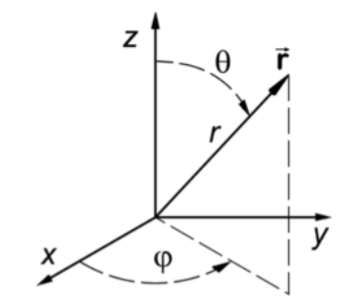
\includegraphics[scale=0.5]{thetaAndPhi.png}
\end{center}


For transformation between cylindrical coordinate and Cartesian coordinate, we have the followings:
$$\hat{r} = \hat{x}\cos(\phi) + \hat{y}\sin(\phi),\quad \hat{\phi} = -\hat{x}\sin(\phi) + \hat{y}\cos(\phi),\quad \hat{z}=\hat{z}$$
$$\hat{x} = \hat{r}\cos(\phi) - \hat{\phi}\sin(\phi),\quad \hat{y}=\hat{r}\sin(\phi) + \hat{\phi}\cos(\phi),\quad \hat{z} = \hat{z}$$
By Chain Rule, we get the following:
$$\frac{d\hat{r}}{dt} = \hat{x}\,(-\sin(\phi)\dot{\phi}) + \hat{y}\,(\cos(\phi)\dot{\phi}) = \dot{\phi}\,\hat{\phi} \qquad\qquad\frac{d\hat{\phi}}{dt} = \hat{x}\,(-\cos(\phi)\dot{\phi})+ \hat{y}\,(-\sin(\phi) \dot{\phi}) = -\dot{\phi}\,\hat{r}$$
Note that $\hat{x},\hat{y},\hat{z}$ are position independent, while $\hat{\phi}$ and $\hat{r}$  are position dependent. \footnote{The basis vector $\hat{r}$ is sometimes denoted as $\hat{\rho}$, or $\hat{s}$.}\\

In general, we have the following transformation between Cartesian and cylindrical coordinate:
$$r = \sqrt{x^2 + y^2} \qquad \qquad \phi = \tan^{-1}\left(\frac{y}{x} \right)\qquad\qquad z=z$$
$$x = r \cos(\phi) \qquad\quad\, \qquad y=r \sin(\phi) \qquad\qquad\quad\,  z=z$$

\hfill\break
For transformation between the spherical coordinate and Cartesian coordinate, we have:
\begin{align*}
&\hat{r} = \hat{x}\sin(\theta) \cos(\phi) + \hat{y}\sin(\theta) \sin(\phi) + \hat{z}\cos(\theta)\\
&\hat{\theta} = \hat{x}\cos(\theta) \cos(\phi) + \hat{y}\cos(\theta)\sin(\phi)  - \hat{z}\sin(\theta) \\ 
&\hat{\phi} = -\hat{x}\sin(\phi) + \hat{y}\cos(\phi)
\end{align*}
\begin{align*}
&\hat{x} = \hat{r}\sin(\theta)\cos(\phi) + \hat{\theta}\cos(\theta) \cos(\phi) - \hat{\phi}\sin(\phi)\\
&\hat{y} = \hat{r}\sin(\theta)\cos(\phi) + \hat{\theta}\cos(\theta)\sin(\phi) + \hat{\phi}\cos(\phi)\\
&\hat{z} = \hat{r}\cos(\theta) - \hat{\theta}\sin(\theta)
\end{align*}
Note that $\hat{x},\hat{y},\hat{z}$ are position independent, while $\hat{\phi}$,$\hat{\theta}$,$\hat{r}$ are position dependent.\\

From such relation one can derive the followings:
\begin{align*}
&\frac{d \hat{r}}{dt} = \dot{\theta}\, \hat{\theta} + \sin(\theta) \dot{\phi}\, \hat{\phi}\qquad\qquad \frac{d\hat{\theta}}{dt}=-\dot{\theta}\,\hat{r}+\cos(\theta)\dot{\phi}\, \hat{\phi}\qquad\qquad \frac{d\hat{\phi}}{dt} = -\sin(\theta)\dot{\phi}\,\hat{r} - \cos(\theta) \dot{\theta}\, \hat{\theta} 
\end{align*}

In general, for transformation between spherical and Cartesian coordinate, we write the following:
$$
x = r \sin(\theta) \cos(\phi) \qquad\qquad y = r \sin(\theta) \sin(\phi) \qquad\qquad z = r\cos(\theta)
$$
$$r = \sqrt{x^2 + y^2 + z^2} \qquad\qquad \theta = \tan^{-1}\left(\frac{y}{x} \right)\qquad\qquad \phi = \tan^{-1}\frac{\sqrt{x^2+y^2}}{z} = \cos^{-1}\frac{z}{\sqrt{x^2+y^2+z^2}}$$


\subsection*{Del Operator}
For a scalar function $T:\R^3 \to \R$, denoted as $T(x,y,z) = T(\vec{r})$. The change in $T$ from the position vector $\vec{r}$ to position vector $\vec{r}+ d\vec{r}$ is given by the following:
$$dT = \frac{\partial T}{\partial x}\,dx + \frac{\partial T}{\partial y}\,dy \frac{\partial T}{\partial z}\,dz = \left( \frac{\pd T}{\pd x}, \frac{\pd T}{\pd y}, \frac{\pd T}{\pd z}\right) \cdot (dx,dy,dz) = \nabla T \cdot d\vec{r}$$
Here $\nabla T$ is a vector and is called the gradient of function $T(\vec{r})$. Note that we have: 
$$dT = \nabla T\cdot d\vec{r} = |\nabla T|\, |d\vec{r}| \, \cos(\theta)$$ where $\theta$ is the angle between $\nabla T$ and $d\vec{r}$, so we see that $dT$ is maximum when $\theta  = 0$, and hence the gradient $\nabla T$ points in the direction of maximum change of function $T$, and its magnitude is the rate of increase along this direction. \\

Now we define the Del operator as the following:
$$\nabla \coloneqq \hat{x}\,\frac{\pd}{\pd x} + \hat{y} \,\frac{\pd}{\pd y}+ \hat{z}\,\frac{\pd}{\pd z}$$

The Divergence of a vector function $\vec{V} =  V_x \hat{x} + V_y \hat{y} + V_z \hat{z}$ is given by the following:
$$\nabla \cdot \vec{V} = \left(\hat{x}\,\frac{\pd}{\pd x} + \hat{y} \,\frac{\pd}{\pd y}+ \hat{z}\,\frac{\pd}{\pd z}\right) \cdot \left( V_x \hat{x} + V_y \hat{y} + V_z \hat{z}\right) = \frac{\pd V_x}{\pd x} + \frac{\pd V_y}{\pd y}+ \frac{\pd V_z}{\pd z}$$
Note that $\nabla \cdot V$ returns a scalar. The divergence is a measure of the spreadness of a vector function. A sink has negative divergence, and a faucet has positive divergence. \\

The Curl of a vector function $\vec{V} =  V_x \hat{x} + V_y \hat{y} + V_z \hat{z}$ is given by the following:
$$\nabla \times \vec{V} = \left( \frac{\pd V_z}{\pd y} - \frac{\pd V_y}{\pd z}\right) \hat{x} + \left( \frac{\pd V_x}{\pd z} - \frac{\pd V_z}{\pd x}\right) \hat{y} + \left( \frac{\pd V_y}{\pd x} - \frac{\pd V_x}{\pd y}\right) \hat{z}$$
Note that $\nabla \times \vec{V}$ returns a vector. Curl is a measure of the curlness, or rotation, of a vector function. The direction of the curl follows the right hand rule.\\

The Laplacian operator is the divergence of gradient. The divergence of gradient of a scalar function $T$ is given by the following:
$$\nabla^2 T \coloneqq \nabla \cdot (\nabla T) = \left(\hat{x}\,\frac{\pd}{\pd x} + \hat{y} \,\frac{\pd}{\pd y}+ \hat{z}\,\frac{\pd}{\pd z}\right) \cdot \left( \frac{\pd T}{\pd x}\hat{x} + \frac{\pd T}{\pd y}\hat{ y} + \frac{\pd T}{\pd z}\hat{z}\right) = \frac{\pd^2 T}{\pd x^2} +  \frac{\pd^2 T}{\pd y^2} + \frac{\pd^2 T}{\pd z^2}$$

Moreover, we note that the curl of gradient of a scalar function $T$ is $\nabla \times (\nabla T) = 0$.\\ 
The gradient of divergence of a vector function $V$ is $\nabla (\nabla \cdot \vec{V})$, but rarely occur in physical problems. \\
The divergence of the curl of a vector function $V$ is given by $\nabla \cdot (\nabla \times \vec{V}) = 0$. \\
The curl of the curl of a vector function $V$ is given by $\nabla \times (\nabla \times \vec{V}) = \nabla ( \nabla \cdot \vec{V}) - \nabla^2 \vec{V}$. \\

The Del operator in cylindrical coordinate system has the following form:
\begin{align*}
\nabla = \hat{\rho}\, \frac{\pd}{\pd r}+ \hat{\phi}\,\frac{1}{r}\frac{\pd}{\pd \phi} + \hat{z}\,\frac{\pd}{\pd z}
\end{align*}
The Del operator in spherical coordinate system has the following form:
\begin{align*}
\nabla = \hat{ r }\, \frac{\pd}{\pd r} +\hat{\theta}\, \frac{1}{r} \frac{\pd}{\pd \theta} + \hat{\phi}\, \frac{1}{r\sin(\theta)} \frac{\pd }{\pd \phi}
\end{align*}

\subsection*{Multivariate Integration}
Line integrals are integrals along lines of path, then come in different forms, with scalar-valued function $f$ and vector-valued function $\vec{V}$:
$$\int_{\vec{a}}^{\vec{b}} f(\vec{r})\, dl, \ \quad \int_{\vec{a}}^{\vec{b}} \vec{V}(\vec{r})\, dl,\ \quad
\int_{\vec{a}}^{\vec{b}} f(\vec{r})\, d\vec{l}, \ \quad	
\int_{\vec{a}}^{\vec{b}} \vec{V}(\vec{r})\, d\vec{l},$$
Here $\vec{a}$ and $\vec{b}$ are the position vectors of the starting and ending points. For a closed path, one has $\vec{a} = \vec{b}$, and the integrals are written as:
$$\oint f(\vec{r})\, dl, \ \quad \oint \vec{V}(\vec{r})\, dl,\ \quad
\oint f(\vec{r})\, d\vec{l}, \ \quad	
\oint \vec{V}(\vec{r})\, d\vec{l},$$
In Cartesian coordinates, we have $d\vec{l} = dx \hat{x} + dy \hat{y} + dz \hat{z}$.
$$\int_{\vec{a}}^{\vec{b}} dl = \text{length of the path} \qquad \qquad \qquad \oint dl = \text{circumference of the path}$$
$$\int_{\vec{a}}^{\vec{b}} d\vec{l} = \vec{b} - \vec{a}\qquad\qquad \qquad \oint d\vec{l} = 0$$
Surface integrals are integrals over surfaces and have the forms given by:
$$\int_S f(\vec{r})\, da, \ \quad \int_S f(\vec{r})\, d\vec{a}, \ \quad \int_S \vec{V}(\vec{r}) \, da,\ \quad \int_S \vec{V}(\vec{r})\cdot d\vec{a}, \ \quad \int_S \vec{V}(\vec{r})\times d\vec{a}$$
Here $da$ and $d\vec{a}$ are scalar and vector infinitesimal surface areas, respectively. $d\vec{a}$ has direction perpendicular to the surface, which has two possibilities for an open surface. By convention, $d\vec{a}$ points outwards for a closed surface. In Cartesian coordinates, we have: $$d\vec{a} = dydz \hat{x} + dzdx \hat{y} + dxdy \hat{z}$$
$\int_S \vec{V}\cdot d\vec{a}$ is a measure of the flow, or the flux, out of the surface $S$.\\
$\int_S\, da$ gives the  area of the surface $S$.\\
$\int_S\, d\vec{a}$ gives the vector surface area.\\

Volume integrals are integrals over volumes given by the forms:
$$\int_V f(\vec{r})\, d\tau,\ \qquad \qquad \int_V \vec{V}(\vec{r})\, d\tau$$
Here $d\tau$ is the infinitesimal volume element. In Cartesian coordinates, we have $d\tau = dx\, dy\, dz$. \\
$\int_V\, d\tau$ gives the volume of the object $V$. \\

\begin{thm}[The Fundamental Theorem for Gradients]
For $1$-dimensional function $f$, we have $\int_a^b \frac{df}{dx}\, dx = f(b) - f(a)$.\\
For $3$-dimensional scalar-valued function $T$, we have $\int_{\vec{a}}^{\vec{b}} \nabla T(\vec{r})\cdot d\vec{l} = T(\vec{b}) - T(\vec{a})$
\end{thm}

Here we see that $\int_{\vec{a}}^{\vec{b}} \nabla T(\vec{r})\cdot d\vec{l}$ is independent of the path taken, so $\oint \nabla T(\vec{r})\cdot d\vec{l} = 0$ for closed path.\\

\begin{thm}[Divergence Theorem]
For $3$-dimensional vector-valued function $\vec{V}$, and an object $V$, we have $\int_V (\nabla \cdot \vec{V})\, d\tau = \oint_S \vec{V}\cdot d\vec{a}$
\end{thm}
Theorem 1.2 is sometimes called the Gauss's Theorem, which states that the volume integral of a divergence is equal to the vector integral of the function over the surface of the volume. Theorem 1.2 is also a statement of the conservation, one can view $\int_V (\nabla \cdot \vec{V})\, d\tau$ as a measure of the sum the source inside the volume, and $\oint_S \vec{V}\cdot d\vec{a}$ as a measure of the flow out of the surface boundary of the object.\\

\begin{thm}[Stokes' Theorem]
For $3$-dimensional vector valued function $\vec{V}$, and a surface $S$, we have $\int_S (\nabla\times \vec{V}) \cdot d\vec{a} = \oint \vec{V}\cdot d\vec{l}$
\end{thm}
The integral of a curl over a surface is equal to the line integral of the function along the boundary of the surface. The surface and the line directions follow the right hand rule. From Theorem 1.3, we see that $\int_S (\nabla\times \vec{V}) \cdot d\vec{a}$ only depends on the boundary line, not the surface used, and hence $\oint_S (\nabla\times \vec{V}) \cdot d\vec{a} = 0$ for any closed surface, the boundary line of closed surfaces shrink to a point. 


\newpage
\section[Fourier Series]{\color{red} Fourier Series\color{black}}
Fourier series is named after French mathematician Jean Baptiste Fourier (1786-1830) 
who explained how the principle of superposition can be used to analyze non-sinusoidal waves.\\

\begin{thm}
Any reasonable real-valued function $f$ over $[-\pi,\pi]$ can be decomposed in terms of Fourier Series:
$$f(x) = \frac{a_0}{2}+\sum_{n=1}^\infty \left( a_n \cos(nx) + b_n \sin(nx)\right)$$
where we have:
$$a_n = \frac{1}{\pi}\int_{-\infty}^{\infty} f(x)\cos(nx) \, dx \qquad\qquad\qquad\qquad b_n = \frac{1}{\pi}\int_{-\pi}^{\pi} f(x) \sin(nx) \, dx$$
\end{thm}
Theorem 3.1.1 is based on the property that $\{1, \sin(nx), \cos(nx) \mid n \in \N\}$ is a complete and orthogonal set, where we can write:
\begin{align*}
\int_{-\pi}^{\pi} \sin(mx)\sin(nx)\, dx = \pi \delta_{mn} \qquad \int_{-\pi}^{\pi} \cos(mx)\cos(nx)\, dx = \pi \delta_{mn} \qquad \int_{-\pi}^{\pi} \sin(mx) \cos(nx) \, dx = 0 
\end{align*}
For a function over $[-L,L]$, the Fourier Series can be recasted as the following:
\begin{align*}
f(x) = \frac{a_0}{2} + \sum_{n=1}^\infty \left( a_n \cos\left( \frac{n\pi x}{L}\right) + b_n \sin\left( \frac{n \pi x}{L}\right) \right)
\end{align*}
where we define:
\begin{align*}
a_n = \frac{1}{L}\int_{-L}^{L} f(x) \cos\left( \frac{n\pi x}{L}\right)\, dx \quad\qquad\qquad\qquad b_n = \frac{1}{L}\int_{-L}^L f(x) \sin\left(\frac{n\pi x}{L}\right)\, dx 
\end{align*}
and the orthogonal integral identities given by:
\begin{align*}
\int_{-\pi}^{\pi} \sin(mkx)\sin(nkx)\, dx = \pi \delta_{mn} \quad
\int_{-\pi}^{\pi} \cos(mkx)\cos(nkx)\, dx = \pi \delta_{mn} \quad
\int_{-\pi}^{\pi} \sin(mkx) \cos(nkx) \, dx = 0 
\end{align*}
where $k = \frac{\pi }{L}$. Depending on applications, the series may involve only sine or cosine.\\


\hfill\break
\hfill\break
Now suppose a set of functions $\mathcal{G} = \{g_n(x)\mid n \in \N\}$, is complete and orthogonal over a range $[0,a]$. Then we can write:
\begin{align*}
\int_0^a g_m(x)\, g_n(x) \, dx = G \delta_{mn} = \begin{cases}G & m = n \\ 0 & m\neq n \end{cases}
\end{align*}
where $G$ is a constant, called the normalization. Any other reasonable function $f(x)$ over the range $[0,a]$ can be decomposed as a linear summation of functions in $\mathcal{G}$. That is, we have:
$$f(x) = \sum_n c_n g_n(x)$$
To calculate the coefficient $c_n$, if $f(x)$ is known, one can write the following:
\begin{align*}
\int_0^a f(x) g_m(x) \, dx = \sum_n c_n \int_0^a g_m(x) g(x) \, dx = \sum_n c_n G\,\delta_{mn} = G\,c_m
\end{align*}
It follows that:
\begin{align*}
c_n = \frac{1}{G} \int_0^a f(x)\, g_n(x)\, dx = \frac{\int_0^a f(x)\, g_n(x)\, dx}{\int_0^a g_n(x)\, g_n(x)\, dx}
\end{align*}

Note that this procedure is the same as the extraction of coordinate components of a vector function $\vec{V} = V_x\hat{x}+V_y\hat{y}+V_z \hat{z}$, except the bases for vector spaces, $\hat{x},\hat{y}$ and $\hat{z}$, are normalized:
\begin{align*}
V_x = \frac{\vec{V}\cdot \hat{x}}{\hat{x}\cdot \hat{x}} = \vec{V}\cdot \hat{x}\quad\Rightarrow\quad \vec{V}\hat{x}
\end{align*}
\newpage

\section[Legendre Differential Equation and Polynomials]{\color{red}Legendre Differential Equation and Polynomials\color{black}}
Legendre differential equations and polynomials are named after French mathematician Adrien-Marie Legendre (1752-1833).

\begin{defn}
The Legendre Differential Equation of $l$-th order is of the following form:
\begin{align*}
\frac{d}{dx}\left( (1-x^2) \frac{dy}{dx}\right) + l(l+1)y = 0
\end{align*}
with $|x|\leq 1$.
\end{defn}

In general, the solution to the $l$-th order Legendre differential equation is singular at $|x| = 1$. However, for integer $l$, the solution is regular and is described by the Legendre polynomials given by the Rodrigues Formula:
\begin{align*}
P_l(x) = \frac{1}{2^l l!}\left( \frac{d^l}{dx^l} (x^2 -1)^l \right)
\end{align*}
The Legendre polynomials are orthogonal and complete. That is, we can write the following:
\begin{align*}
\int_{-1}^{1} P_m(x) \, P_n(x) \, dx = \frac{2}{2m+1}\delta_{mn}
\end{align*}

Any piecewise continuous function $f(x)$ with a finite number of discontinuities in the interval $[-1,1]$ can be written as the summation of the following form:
\begin{align*}
f(x) = \sum_{l=0}^\infty a_l P_l(x)
\end{align*}
with $a_l$ being constant defined by:
\begin{align*}
a_l = \frac{2l+1}{2}\int_{-1}^1 f(x)P_l(x)\, dx
\end{align*}

\hfill\break
\hfill\break
\note Here we have the Bonnet's Recursive Formula:
\begin{align*}
(l+1) P_{l+1}(x) = (2l+1)x\, P_l(x) - l\, P_{l-1}(x)
\end{align*}

\hfill\break
\hfill\break
In the angular form, that is, if $x = \cos(\theta)$, the orthogonality conditions are given by the following:
\begin{align*}
\int_0^\pi P_m(\cos(\theta)) P_n(\cos(\theta))\, \sin(\theta) \, d\theta = \frac{2}{2m+1}\, \delta_{mn}
\end{align*}
and the function decomposition is given by the following:
\begin{align*}
f(\theta) = \sum_l a_l P_l(\cos(\theta)) \qquad\qquad\text{with }a_l=\frac{2l+1}{2}\int_0^{\pi} f(\theta) P_l(\cos(\theta) \sin(\theta) \, d\theta 
\end{align*}



\newpage
\chapter{Electrostatics}
\begin{thm}
Coulomb's Law is named after French physicist Charles-Augustin de Coulomb (1736-1806). The electric force on a test charge $Q$ at $\vec{r}$ due to a source charge $q$ at $\vec{r}'$ at rest is given by the following:
\begin{align*}
\vec{F}(\vec{r})  = \frac{qQ}{4\pi \epsilon_0}\frac{\vec{r} - \vec{r}'}{\left|\vec{r} - \vec{r}'\right|^3}
\end{align*}
where we have the constant $\epsilon_0 = 8.85\cdot 10^{-12} \, \frac{C^2}{n\cdot m^2}$ is called the permittivity of the free space. \\
\end{thm}
\note Coulomb's Law is a fundamental law of physics, and cannot be derived from other laws. 
\hfill\break
\hfill\break
\hfill\break
\hfill\break
\hfill\break
\section[Electric Field]{\color{red}Electric Field\color{black}}
\begin{defn}
Electric field at a point is defined to the be force per unit test charge at this point, hence we write:
\begin{align*}
\vec{E}(\vec{r}) = \frac{F(\vec{r})}{Q} = \frac{q}{4\pi \epsilon_0} \frac{\vec{r} - \vec{r}'}{\left|\vec{r} - \vec{r}'\right|^3}
\end{align*}



The force obeys the principle of superposition, so does the electric field. \\For multiple source charge $q_i$, at location $\vec{r}_i$, we can write:
$$\vec{E}(\vec{r}) = \sum_i \vec{E}_i (\vec{r}) = \sum_i \frac{q_i}{4\pi \epsilon_0}\frac{\vec{r} - \vec{r}'}{\left|\vec{r}-\vec{r}_i\right|^3}$$
The unit of electric field is given by:
$$\frac{\text{Newton}}{\text{Coulumb}} = \frac{N}{C}$$
\end{defn}
\hfill\break
\begin{center}
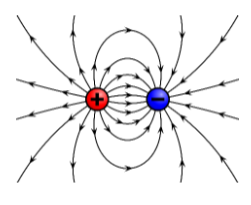
\includegraphics[scale=0.8]{electricField.png}
\end{center}



\newpage
\subsection*{Continuous charge distributions}
For a continuous charge distribution of charges, the summation of charges becomes an integral:
$$\sum_i q_i = \int dq$$

The electric field at location $\vec{r}$ due to this continuous charge distribution is then given by:
$$\vec{E}(\vec{r}) = \frac{1}{4\pi \epsilon_0}\int \frac{\vec{r}-\vec{r}'}{\left|\vec{r}-\vec{r}'\right|^3}dq$$
The integral for electric field depends on the charge distribution over an object:
\begin{enumerate}[topsep=3pt,itemsep=-1ex,partopsep=1ex,parsep=1ex]
\item Over a line, that is, a line charge, we have $dq = \lambda(\vec{r}') dl'$, where $\lambda$ is the charge per unit length
\item Over a surface, that is, a surface charge, $dq = \sigma(\vec{r}') da'$, where $\sigma$ is charge per unit area
\item Over a volume, that is, a volume charge, $dq = \rho(\vec{r}')d\tau'$, where $\rho$ is charge per unit volume
\end{enumerate}

\begin{center}
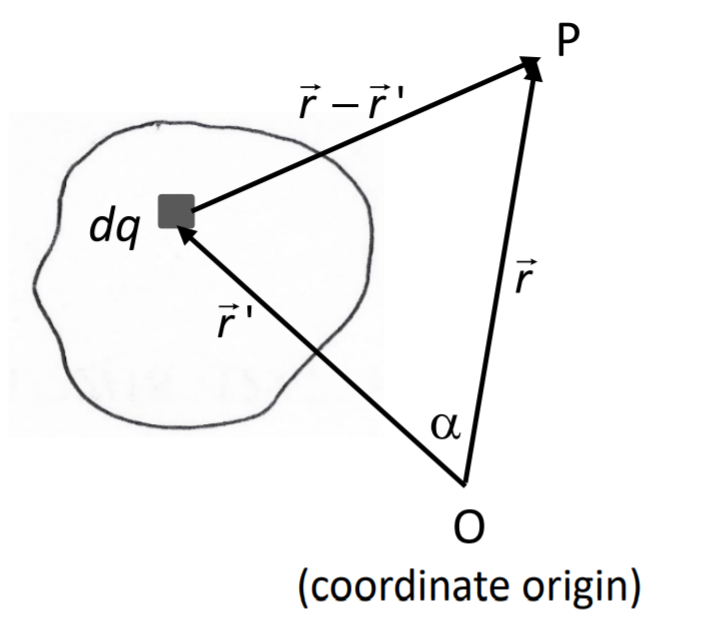
\includegraphics[scale=0.3]{multipoleExpansions.png}
\end{center}

Here $\lambda, \sigma, \rho$ are called line, surface, and volume charge densities, respectively. The primed superscripts indicate the integrating variables. For a special case, say the charge density of a point charge $q$ at $\vec{a}$, we have $\rho (\vec{r}') = q\delta^3 (\vec{r}'-\vec{a})$, where we can write:
$$\vec{E}(\vec{r}) = \frac{1}{4\pi \epsilon_0} \int \frac{\vec{r}-\vec{r}'}{\left| \vec{r}-\vec{r}'\right|^3} q\delta^3(\vec{r}'-\vec{a})d\tau' = \frac{q}{4\pi \epsilon_0}\frac{\vec{r}-\vec{a}}{\left|\vec{r}-\vec{a}\right|^3}$$

For a source charge $q$ at the origin, the electric field at position $\vec{r}$ is given by:
$$\vec{E}(\vec{r}) = \frac{q}{4\pi \epsilon_0 }\frac{\vec{r}}{|\vec{r}|^3} = \frac{q}{4\pi \epsilon_0 |\vec{r}|^2} \hat{r}$$
\begin{defn}
Electric field lines are lines with arrows representing the direction of the electric field. The perpendicular surface density of the lines represents the strength of the field. The field lines originate from positive charges, and terminate at negative charges. 
\end{defn}

\begin{defn}
Electric field flux is a measure of the total field lines through a surface, even though one cannot measure the number of electric field lines. Hence the electric field flux is defined by the following:
$$\Phi = \int \vec{E}\cdot d\vec{a}$$
\end{defn}
\begin{center}
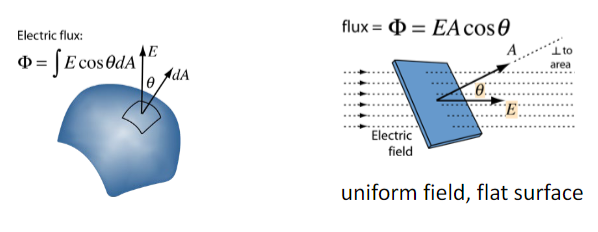
\includegraphics[scale=0.8]{flux.png}
\end{center}


\begin{thm}
Gauss's Law is named after German mathematician Carl Friedrich Gauss (1777-1855). For a point charge $q$ at the origin, the total flux through a closed surface $S$ enclosing the origin is given by:
$$\oint_S E\cdot d\vec{a} = \oint_S\left(\frac{1}{4\pi\epsilon_0}\frac{q}{r^2}\hat{r}\right)\cdot (r^2 d\Omega \hat{r}) = \frac{q}{4\pi \epsilon_0}\oint_S d\Omega = \frac{q}{\epsilon_0}$$
\end{thm}


For multiple charges at different locations, the total flux through a surface $S$ that encloses all these charges is given by the following:
$$\oint_S \vec{E}\cdot d\vec{a} = \int_i \oint_S \vec{E}_i \cdot d\vec{a} = \sum_i \frac{q_i}{\epsilon_0} = \frac{Q_{enclosed}}{\epsilon_0} \qquad \Rightarrow \qquad \oint_S \vec{E}\cdot d\vec{a} = \frac{Q_{enclosed}}{\epsilon_0}$$
where we have:
$$Q_{enclosed} = \sum_i q_i \text{ is the total charge inside the surface }S$$
The closed surface is often called the Gaussian surface.\\

For a continuous charge distribution and using the divergence theorem, we get the following:
$$Q_{enclosed} = \int \rho\, d\tau, \quad \oint_S \vec{E}\cdot d\vec{a} = \int_V (\nabla \cdot \vec{E}) d\tau \qquad \Rightarrow \qquad \int (\nabla \cdot \vec{E}) d\tau = \frac{1}{\epsilon_0} \int \rho d\tau$$
which is true for any volume, which leads to the differential form of the Gauss's Law:
$$\nabla \cdot \vec{E}(\vec{r}) = \frac{\rho(\vec{r})}{\epsilon_0}$$

\note Gauss's Law does not offer anything fundamentally new, it is derived from Coulomb's Law.\\

Electric field calculations for certain symmetric geometries can be greatly simplified by applying the integral form of the Gauss's Law if we have the following holds:
$$\int \vec{E} \cdot d\vec{a} = \int E\, da = E \int da$$

\subsection*{The curl of the electric field}
Consider a point charge $q$ at the origin. For point $\vec{a}$ and $\vec{b}$ in the space, with distance $r_a$ and $r_b$, respectively, from the origin, we get the following holds:
$$\int_{\vec{a}}^{\vec{b}}  \vec{E}\cdot d\vec{l} = \int_{\vec{a}}^{\vec{b}} \left( \frac{1}{4\pi \epsilon_0}\frac{q}{|\vec{r}|^2}\hat{r}\right) \cdot \left(dr\, \hat{r}+rd\theta\, \hat{\theta} + r\sin(\theta) d\phi\, \hat{\phi}\right) = \frac{q}{4\pi \epsilon_0}\int_{\vec{a}}^{\vec{b}} \frac{dr}{r^2} = \frac{q}{4\pi \epsilon_0}\left( \frac{1}{r_a}-\frac{1}{r_b}\right)$$
\begin{center}
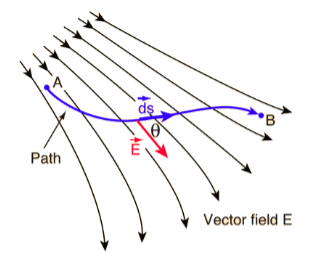
\includegraphics[scale=0.8]{curlE.png} \footnote{Note that $d\vec{s}$ in the figure is $d\vec{l}$ in our derivation.}
\end{center}

which depends only on $r_a$ and $r_b$, independent of the path. Hence for a closed path $l$, with $r_a = r_b$, we can write:
$$\oint_l \vec{E}\cdot \vec{l} = 0$$
by Stoke's Theorem, this implies that we have:
$$\nabla \times \vec{E} = 0$$
We assumed that the point charge is at the origin for the convenience of derivation, but the results hold no matter where the charge is located. Moreover, from the principle of superposition, we can write the following:
$$\vec{E} = \vec{E}_1 + \vec{E}_2 +\cdots = \sum_i \vec{E}_i \qquad \Rightarrow \qquad \nabla \times \vec{E} = \sum_i \nabla \times \vec{E}_i = 0$$
for any charge distribution.\\

Here we conclude the following:
\begin{thm}
The electric field from any static charge distribution is curl-less, that is, we write:
$$\nabla \times \vec{E} = 0$$
\end{thm}

\newpage
\section[Electric Potential]{\color{red} Electric Potential \color{black}}
Since we have $\nabla \times \vec{E} = 0$, by mathematical argument, the electric field can always be expressed as a gradient of a scalar potential, denoted as $V(\vec{r})$, in which case we can define the following:
$$-\nabla V(\vec{r}) \coloneqq \vec{E}(\vec{r})$$
Here we note that $\vec{E}(\vec{r})$ points int the direction of the maximum decrease in $V(\vec{r})$. From the fundamental theorem of gradient, we can write the following:
\begin{align*}
 \int_{\vec{a}}^{\vec{b}} \vec{E}\cdot d\vec{l} = -\int_{\vec{a}}^{\vec{b}} \nabla V\cdot d\vec{l} = -\left( V(\vec{b}) - V(\vec{a})\right) \qquad \Rightarrow \qquad V(\vec{b}) - V(\vec{a}) = -\int_{\vec{a}}^{\vec{b}} \vec{E}\cdot d\vec{l}
\end{align*}
If the location $\vec{a}$ is chosen as the reference point such that $V(\vec{a}) = 0$, denoting such point as $O$, then the potential at any point $\vec{r}$ is uniquely determined by the following:
\begin{align*}
V(\vec{r}) = -\int_O^{\vec{r}}\vec{E}\cdot d\vec{l}
\end{align*}
\begin{defn}
The potential difference between two points in space is called the voltage.
\end{defn}

\remark For a localized charge distribution, that is, the distribution does not extend to infinity, it is conventional to set $V= 0$ at infinity. In reality, the ground is assumed to have $V=0$. While for a charge distribution extending to infinity, setting $V=0$ is often not possible. \\

\note Following the superposition properties of the electric field, the electric potential obeys the superposition principle:
$$\vec{E} = \sum_i \vec{E}_i \qquad \qquad \Rightarrow \qquad \qquad V = \sum_i V_i$$
The unit for potential is measured in Volt, denoted as $V$, where we have:
$$1\, V = 1\, J/C$$
with such definition of Volt, the electric field also has a new unit $V/m$. \\

\subsection*{Potential of a charge distribution}
For a point charge $q$ at the origin, the potential at $\vec{r} $ is given by the following:
\begin{align*}
V(\vec{r}) = -\int_O^{\vec{r}} \vec{E}\cdot d\vec{l} = -\int_{\infty}^r \left(\frac{1}{4\pi \epsilon_0}\frac{q}{r^2}\hat{r}\right)\cdot \left( dr\, \hat{r}\right) = \frac{1}{4\pi \epsilon_0}\frac{q}{r}
\end{align*}
If the point charge is instead at $\vec{r}'$, then the potential at $\vec{r}$ is then given by:
$$V(\vec{r}) = \frac{1}{4\pi \epsilon_0}\frac{q}{||\vec{r}-\vec{r}'||}$$
Then for multiple charges $q_i$ at locations $\vec{r}_i$, we can write the following:
\begin{align*}
V(\vec{r}) = \sum_i V_i(\vec{r}) = \frac{1}{4\pi \epsilon_0}\sum_i \left(\frac{q_i}{||\vec{r} - \vec{r}_i||} \right)
\end{align*}
For a continuous localized charge distribution, we can write the following:
\begin{align*}
\sum_i q_i = \int dq \qquad \qquad \Rightarrow \qquad \qquad V(\vec{r}) = \frac{1}{4\pi \epsilon_0}\int \frac{dq}{||\vec{r}-\vec{r}'||}
\end{align*}
where we have the following holds:
\begin{enumerate}[topsep=3pt,itemsep=-1ex,partopsep=1ex,parsep=1ex]
\item $dq = \lambda dl'$ for line charge and line charge density $\lambda$. 
\item $dq = \sigma da'$ for surface charge and surface charge density $\sigma$.
\item $dq = \rho d\tau'$ for volume charge and volume charge density $\rho$. 
\end{enumerate}
Here $l'$, $a'$, and $\tau'$ are integral variables.\\

\note The potential encodes all the information about an electric field. Since potential is a scalar function, it is easier to be dealt with mathematically than vector field $E$.\\

\remark For a charge distribution extending to infinity, the integral diverges because it assumes the potential vanishes at infinity, which is not possible in such case. 


\newpage
\begin{defn}
Equipotential surfaces are surfaces with constant potential, which are perpendicular to the electric field. The electric field points in the direction of the decreasing potential. 
\end{defn}
\begin{center}
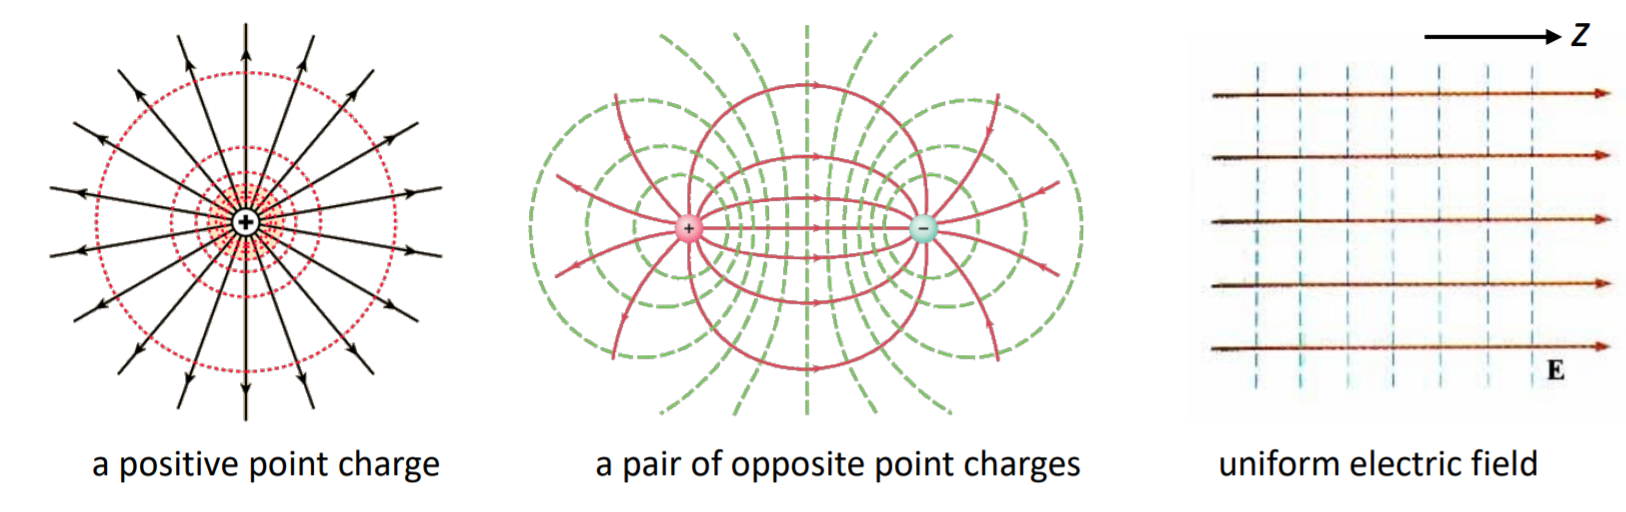
\includegraphics[scale=0.3]{equipotential.png}
\end{center}

\subsection*{Potential of a uniform field}
For a uniform field, say, point in the $z$-direction, with $\vec{E} = E_0 \hat{z}$. We can write the following:
\begin{align*}
V(\vec{r}) = -\int_O^{\vec{r}}\vec{E}\cdot d\vec{l} = - \int_O^z E_0 dz
\end{align*}
The reference point $O$ cannot be at the infinity. Since any plane perpendicular to the $z$-axis is an equipotential surface, it is convenient to choose $V=0$ at $z=0$. In such case, we can write:
\begin{align*}
 V(\vec{r}) = -E_0 z
\end{align*}


\subsection*{Poisson's Equation and Laplace's Equation}
Poisson's Equation and Laplace's Equation are named after French mathematicians Simeon Denis Poisson (1781-1840) and Pierre-Simon Laplace (1749-1827). \\

The electric field can be expressed as a gradient of a scalar potential $\vec{E} = -\nabla V$, and has the divergence and curl $\nabla \cdot \vec{E} = \frac{\rho}{\epsilon_0}$, and $\nabla \times \vec{E} = 0$. Note that the curl-lless is automatically satisfied by $\vec{E} = -\nabla V$ since $\nabla \times (\nabla V) = 0$. Rewrite the Gauss's Law using the potential, we get:
\begin{align*}
\nabla^2 V(\vec{r}) = -\frac{\rho (\vec{r})}{\epsilon_0} \tag{P}
\end{align*}
here equation (P) is known as the Poisson's Equation. \\
For regions without charge, the equation becomes the following:
\begin{align*}
\nabla^2 V(\vec{r}) = 0 \tag{L}
\end{align*}
here equation (L) is known as the Laplace's Equation.\\

In particular, charge distributions are not known and not easily measurable.  Often potentials can be measured in some regions, then the problem becomes solving differential equations with boundary conditions.\\
\hfill\break
\begin{center}
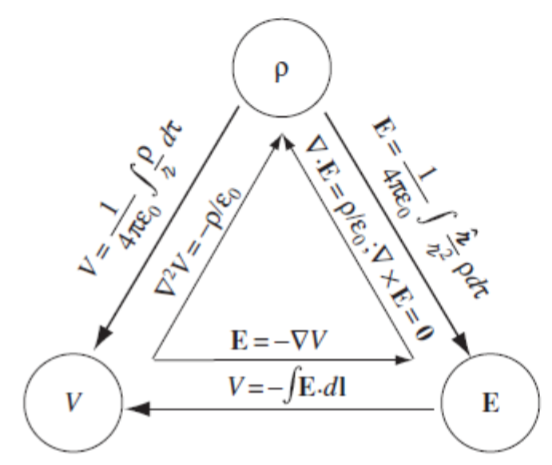
\includegraphics[scale=0.6]{VErho.png}
\end{center}

\newpage
\section[Boundary Conditions]{\color{red}Boundary Conditions\color{black}}
One might have noticed that the potential is always continuous while the electric field 
discontinues at boundaries of surface charges. Since $\vec{E} = -\nabla V$ the potential must be continuous, otherwise the gradient is not defined , and hence we would have infinite electric field. \\

\begin{center}
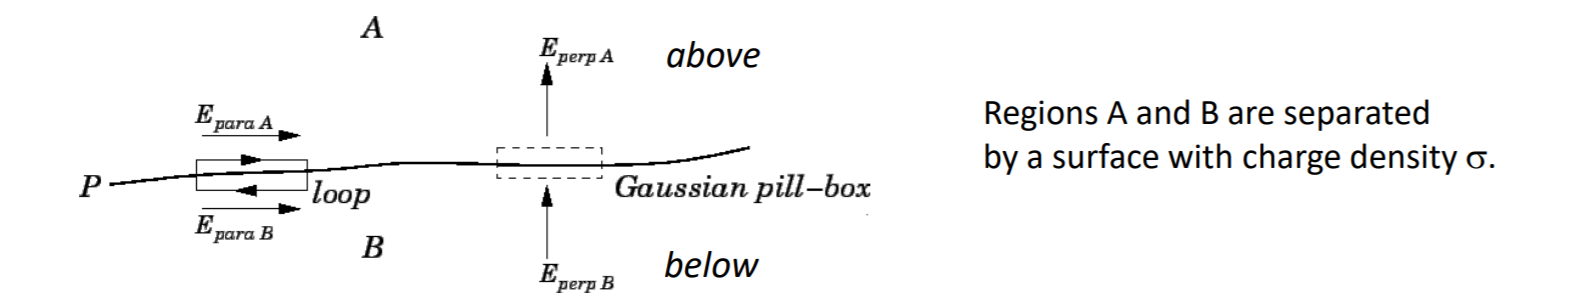
\includegraphics[scale=0.39]{Epara.png}
\end{center}

Consider $P$ being a charged surface of charge density $\sigma$. Here we take a line integral over an infinitesimal rectangular loop $L$ across the surface, we obtain the following:
\begin{align*}
\oint_L \vec{E}\cdot d\vec{l} = 0 \qquad \Rightarrow \qquad (E_{para\, B} - E_{para\, A})\cdot (length) = 0\qquad \Rightarrow\qquad E_{para\, B} = E_{para\, A}
\end{align*}
The tangential component of the electric field is always continuous. \\

On the other hand, we can take a surface integral over an infinitesimal Gaussian pill-box $S$ across the surface, we obtain the following:
\begin{align*}
\oint_S \vec{E}\cdot d\vec{a} = \frac{q}{\epsilon_0} \quad \Rightarrow \quad (E_{perp\, A} - E_{perp\, B})\cdot (Area) = \frac{\sigma\cdot (Area )}{\epsilon_0} \qquad \Rightarrow\qquad E_{perp\, A} - E_{perp\, B} = \frac{\sigma}{\epsilon_0}
\end{align*}
The normal component of the electric field discontinues across a surface charge.\\

Now we define region $A$ as above and region $B$ as below the surface charge, the two boundary conditions can be combined into one equation:
$$\vec{E}_{above} - \vec{E}_{below} = \frac{\sigma}{\epsilon_0}\vec{n}$$
where $\vec{n}$ is the unit vector normal to the surface, pointing from below to above. As the path shrinks to zero, the change in potential across the boundary vanishes, hence we have $V_{above} - V_{below} = -\int_{below}^{above} \vec{E}\cdot d\vec{l} = 0 \Rightarrow V_{above} = V_{below}$. Hence we see that the potential is continuous across any boundary. However, the derivative of the potential inherits the discontinuity from $\vec{E}$, that we have $\vec{E}_{above} - \vec{E}_{below} = \frac{\sigma}{\epsilon_0}\vec{n} \Rightarrow \nabla V_{above} - \nabla V_{below} = \frac{\sigma}{\epsilon_0}\vec{n}$. Concluding we get:
\begin{align*}
\frac{\partial V_{above}}{\partial n} - \frac{\partial V_{below}}{\partial n} = -\frac{\sigma}{\epsilon_0}
\end{align*}








\newpage
\section[Work and Energy]{\color{red}Work and Energy\color{black}}
If a charge is $Q$ is move slowly from position $\vec{a}$ to position $\vec{b}$, one needs to exert a force to overcome the electric force. Therefore, the work done to the charge is given by the following:
\begin{align*}
W = \int_{\vec{a}}^{\vec{b}} \vec{F}\cdot d\vec{l} = \int_{\vec{a}}^{\vec{b}}(-Q\vec{E}) \cdot d\vec{l} = Q(V(\vec{b}) - V(\vec{a})) \qquad \Rightarrow \qquad V(\vec{b}) - V(\vec{a}) = \frac{W}{Q}
\end{align*}
Thus, the potential difference between points $\vec{b}$ and $\vec{a}$ is equal to the work per unit charge required to move the charge from $\vec{a}$ to $\vec{b}$.\\

Now suppose the charge is moved from infinity to position $\vec{r}$, then the work done is given by:
$$W = Q(V(\vec{r}) - V(\infty)) = Q(\vec{r})$$
which turns into the potential energy of the charge in the electric field, denoted as $U$. Thus the potential is the potential energy per unit charge. \\

Now suppose we want to assemble two point charges from infinity. It takes not work to bring in the first charge $q_1$. However, work is needed to be done to bring in the second charge $q_2$ to overcome the electric force due to the first charge. Hence the work done is given by the following:
\begin{align*}
W = q_2 V_1(\vec{r}_2) = q_2 \frac{1}{4\pi \epsilon_0}\frac{q_1}{||\vec{r}_2 - \vec{r}_1||} = \frac{q_1q_2}{4\pi \epsilon_0 ||\vec{r}_2 - \vec{r}_1||}
\end{align*}
which is the electric potential energy between the two charges.\\


\subsection*{Potential Energy of a Point Charge Distribution}
Now extend to multiple point charges, the total work needed to assemble the charge distribution is then given by the following:
\begin{align*}
W = \frac{1}{4\pi \epsilon_0}\sum_i^n \sum_{j>i}^n \frac{q_iq_j}{||\vec{r}_i-\vec{r}_j} = \frac{1}{8\pi \epsilon_0}\sum_{i}^n \sum_{j\neq i} \frac{q_i q_j}{||\vec{r}_i - \vec{r}_j||}
\end{align*}
Rearranging, we get the following:
\begin{align*}
W = \frac{1}{2}\sum_i^n q_i \left( \sum_{j\neq i}^n \frac{1}{4\pi \epsilon_0}\frac{q_j}{||\vec{r}_i - \vec{r}_j||}\right) = \frac{1}{2}\sum_i^n q_i V(\vec{r}_i)
\end{align*}
Here $V(\vec{r}_i)$ is the potential at the location of charge $q_i$ due to all other charges in this space. $W$ is the total electric energy stored in the charge configuration, which can be retrived by dismantling the charge distribution. $W$ here is also called the electrostatic energy $U$.\\

\subsection*{Electrostatic Energy of a Continuous Charge Distribution}
For a continuous distribution, we get the following:
\begin{align*}
W = \frac{1}{2}\int V dq
\end{align*}
here $W$ is the energy stored in the charge distribution.\\

For volume charge density, one can write the following:
\begin{align*}
W = \frac{1}{2}\int V\, dq = \frac{1}{2}\int \rho V\, d\tau
\end{align*}
The volume integral can also be expanded to all space as we set $\rho = 0$ outside the charge distribution. Note that the Gauss's Law states that we have $\rho = \epsilon_0 \nabla \cdot \vec{E}$, and by product rule we have $\nabla \cdot (V\vec{E}) = (\nabla V)\cdot \vec{E} + V(\nabla \cdot \vec{E})$. The work can then be expressed as the following:
\begin{align*}
W = \frac{1}{2}\epsilon_0\int (\nabla \cdot \vec{E}) V\, d\tau = \frac{1}{2}\epsilon_0 \int\left(\nabla \cdot (V\vec{E})-(\nabla V) \cdot \vec{E})\right) \, d\tau = \frac{1}{2}\epsilon_0 \oint V\vec{E}\cdot d\vec{a}+\frac{1}{2}\epsilon_0 \int E^2 d\tau
\end{align*}
Here $\oint V\vec{E}\cdot d\vec{a}$ vanishes when we integral over all space for a localized charge distribution. Hence the potential energy stored in such charge distribution over all space can be written as the following:
\begin{align*}
W = \frac{1}{2}\epsilon_0 \int E^2 d\tau
\end{align*}
Now the integral is over all space and the integrand is $E^2$, hence $W$ can be interpreted as the energy stored in the electric field with energy density given by:
$$u_E = \frac{1}{2}\epsilon_0 E^2$$

\hfill\break
Comparing the two methods of the calculation for the electrostatic energy:
\begin{align*}
(1)\ W = \frac{1}{2}\sum_i q_i V(\vec{r}_i) \qquad \qquad \qquad \qquad \qquad (2)\ W = \frac{1}{2}\epsilon_0 \int E^2\, d\tau
\end{align*}
Note here the energy can be negative from method (1), while always positive from method (2).\\
Now consider a single point charge, according to the two methods, (1) gives $W=0$, while (2) gives $W = \frac{1}{2}\epsilon_0 \int E^2\, d\tau = \frac{1}{2}\epsilon_0 \int \left( \frac{1}{4\pi \epsilon_0}\frac{q}{r^2}\right)^2 \, d\tau = \infty$ for integrating the entire space. The reason that causes this inconsistency is that method (1) calculates only the interaction energy between point charges, and it does not include the energy needed to assemble a point charge, often called the self-energy, which is infinity because a point charge is singular. While method (2) includes both self-energy and interaction energy. This point can be further illustrated by the case of two point charges:
$$(1)\ W = \frac{1}{4\pi \epsilon_0}\frac{q_1q_2}{|\vec{r}_1 - \vec{r}_2|}\qquad\qquad\qquad\qquad (2)\ W = \frac{1}{2}\epsilon_0 \int(\vec{E}_1+\vec{E}_2)^2 \, d\tau = \frac{1}{2}\epsilon_0 \int(E_1^2+E_2^2 + 2\vec{E}_1 \cdot \vec{E}_2)\, d\tau$$
The first two integrals in the second method are self-energies of the two point charges. The third integral is the interaction between the two charges, one can show that we have the following:
\begin{align*}
\frac{1}{2}\epsilon_0 \int (2\vec{E}_1\cdot \vec{E}_2) \, d\tau = \frac{1}{4\pi \epsilon_0}\frac{q_1q_2}{|\vec{r}_1 - \vec{r}_2|}
\end{align*}
\note Since work is proportional to the quadratic of the electric fields, then work does not obey the superposition principle. One cannot calculate the energies of individual charge distributions and sum them up to get the total. \\


\newpage
\section[Conductors]{\color{red}Conductors\color{black}}
Materials can be broadly classified into three classes based on their electric properties:
\begin{enumerate}[topsep=3pt,itemsep=-1ex,partopsep=1ex,parsep=1ex]
\item \textbf{Insulator, or dielectrics}. No free electrons, all electrons are bounded; examples: glass.
\item \textbf{Semiconductor}. Limited supply of free electrons; examples: silicon, germanium.
\item \textbf{Conductor}. Unlimited supply of free electrons; examples: metals such as copper, steel.
\end{enumerate}
\hfill\break
Free electrons will respond to electric field, so conductors has the following electrostatic properties:
\begin{enumerate}[topsep=3pt,itemsep=-1ex,partopsep=1ex,parsep=1ex]
\item $\vec{E} = 0$ inside a conductor in equilibrium.\\ 
Free electrons will redistribute to cancel any field inside the conductor. 
\item No net charge density inside the conductor. \\
Following $\rho = \epsilon_0 \nabla \cdot \vec{E}$, any net charge must reside on its surface.
\item A conductor must be at an equipotential. \\
For any two points, $\vec{r}_1, \vec{r}_2$, inside the conductor, we have $V(\vec{r}_2) - V(\vec{r}_1) = -\int_{\vec{r}_1}^{\vec{r}_2} \vec{E}\cdot d\vec{l} = 0$.
\item Just outside a conductor, $\vec{E}$ must be normal to the surface. \\
$\vec{E} = 0$ inside the conductor and $E_{parallel}$ is continuous.
\end{enumerate}
\begin{center}
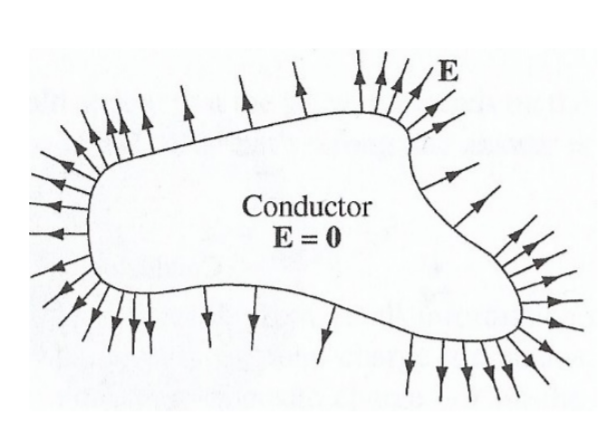
\includegraphics[scale=0.39]{EFieldConductor.png}
\end{center}


No field liens can penetrate the conductor, all file lines must terminate at or originate from the surface of a conductor. The surface charge density can be calculated from the field or potential just outside the conductor:
\begin{align*}
\sigma = \epsilon_0 \vec{E}\cdot \vec{n} = -\epsilon_0 \frac{\partial V}{\partial n}
\end{align*}

Also, from previous results, since the electric field inside a conductor is zero, so we can write:
\begin{align*}
\vec{E}_{outside} - \vec{E}_{inside} = \vec{E}_{outside} = \frac{\sigma}{\epsilon_0}\vec{n}
\end{align*}


\subsection*{Induced Charges}
If a conductor is placed inside an electric field $\vec{E}$, charges will be induced on the surface of the conductor such that the electric field they produce inside the conductor will exactly cancel $\vec{E}$. Hence the net electric field inside the conductor is exactly zero. The field must be zero as well inside a charge-free cavity in the conductor. Moreover, no induced charge can be on the surface of the cavity inside the conductor. 
\begin{center}
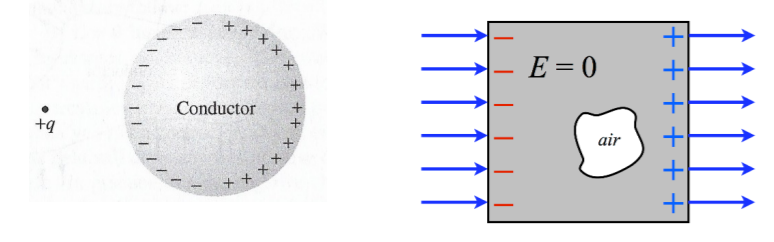
\includegraphics[scale=0.5]{conductors.png}
\end{center}

If there is a charge $+q$ inside a cavity, a total charge $-q$ will be induced on the inner surface of the cavity to terminate all field lines from the charge. By conservation of charge, a total charge $+q$ will be induced on the outer surface of the conductor.
\begin{center}
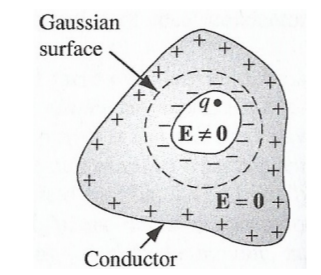
\includegraphics[scale=0.5]{qInCavity.png}
\end{center}

\newpage
Conductor conceals all information about the cavity and the location of the charge inside the cavity. For a spherical outer surface as shown:
\begin{center}
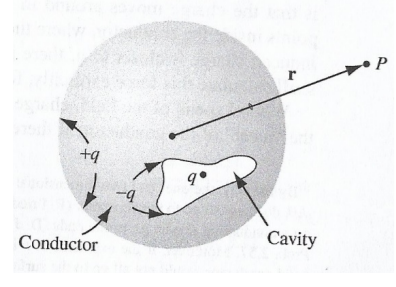
\includegraphics[scale=0.5]{conductorCavity.png}
\end{center}
the induced charge $+q$ will be uniformly distributed, thus the field outside the conductor is the same as that of a point charge $+q$ at the center of the sphere given by the following:
\begin{align*}
\vec{E}(\vec{r}) = \frac{q}{4\pi \epsilon_0}\frac{\vec{r}}{r^3} \qquad (r>R)
\end{align*}

\hfill\break\hfill\break
Note that, if a conductor is placed in an electric field $E$, then there will be induced charge distribution, not necessarily uniform, on the surface of a conductor which creates an electric field $E'$ to cancel out the effect of $E$, so that the electric field inside the conductor $E'+E$ remains zero. That is, a conductor might have non-uniform charge distribution on its surface, and still have zero electric field inside the conductor. 

\hfill\break
\subsection*{Electrostatic Pressure on a Conductor}
Consider a small patch of conductor surface, small enough that it can be treated as a flat surface with a uniform surface charge density of $\sigma$. The small patch of conductor will experience a force due to the electric field of other charges, denoted as $\vec{E}_{other}$. The force per unit area is then given by:
$$\vec{f} = \sigma \vec{E}_{other}$$
Here the other charges include both the surface charges outside the small patch on the conductor and any other charges in the given context.\\

\begin{center}
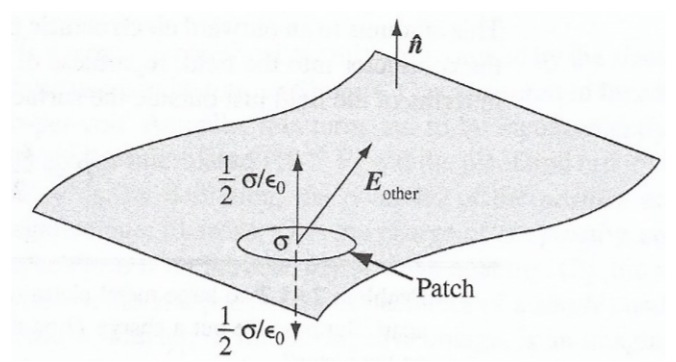
\includegraphics[scale=0.39]{patch.png}
\end{center}

Note that the field inside the conductor is zero and the field immediately outside the conductor is $\sigma/\epsilon\, \vec{n}$, where $\vec{n}$ is the unit normal vector of the patch pointing in the direction to outside the conductor. The fields are the sum of the contributions from the patch itself and the other:
$$\vec{E}_{outside} = \vec{E}_{other} + \frac{\sigma}{2\epsilon_0}\vec{n} = \frac{\sigma}{\epsilon_0}\vec{n}\qquad\qquad\qquad \vec{E}_{inside} = \vec{E}_{other} - \frac{\sigma}{2\epsilon_0}\vec{n} = 0$$
Hence it follows that we have:
$$\vec{E}_{other} = \frac{\sigma}{2\epsilon_0}\vec{n}$$
Thus the force per unit area on the conductor due to the surface charge is given by:
$$\vec{f} = \sigma \vec{E}_{other} = \frac{\sigma^2}{2\epsilon_0}\vec{n}$$
Notice here the force is always pointing outward, away from the conductor, regardless the sign of the surface charge, and such force, per unit area, is called the electrostatic pressure, which tends to draw the conductor into the electric field.\\

Here we can express the electrostatic pressure in terms of the field just outside the conductor:
$$P\coloneqq \frac{\sigma^2}{2\epsilon_0} = \frac{1}{2}\epsilon_0 E^2$$





\newpage
\section[Capacitor]{\color{red}Capacitor\color{black}}
\begin{defn}
A capacitor is an electric device that stores electric charge. It generally consists of two conductors, one with charge $+Q$ and the other with charge $-Q$. 
\begin{center}
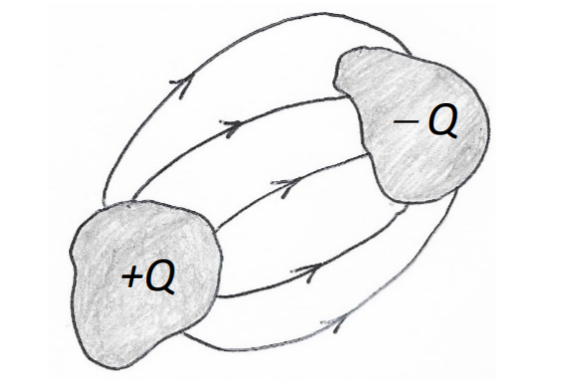
\includegraphics[scale=0.39]{capacitor.png}
\end{center}

The potential difference between the two conductors is given by the following:
$$V = V_+ - V_- = \left(-\int_{(-)}^{(+)} \vec{E}\cdot d\vec{l} \right)\propto Q$$
The proportional constant is called the capacitance:
$$C \coloneqq \frac{Q}{V}$$
\end{defn}

The capacitance $C$ is completely determined by the geometry of the capacitor. The capacitance in measured in farads, denoted as $F$, with $1\, F = 1\, C/V$. \\

Any pair of conductors can be viewed as a capacitor. One piece conductor can also be a capacitor, in such case, the other piece is assumed to be at the infinity.\\

Charging up a capacitor requires moving electrons from one piece of the conductor to another piece, overcoming electric force in the process. The work in moving charge $dq$ is given by:
$$dW = V\, dq = \frac{q}{C}\, dq$$
Hence the total work necessary to charge the capacitor to a total charge $Q$ is given by:
$$W = \int dW = \int_0^Q \frac{q}{C}\, dq = \frac{1}{2}\frac{Q^2}{C} = \frac{1}{2}CV^2$$
Here $V$ is the final potential difference, note that $Q = CV$. $W$ is the energy stored in the charge distribution, or in the electric field of the capacitor, also referred to as $U$.
\begin{align*}
W = \frac{1}{2}\frac{Q^2}{C} = \frac{1}{2}CV^2 \tag{*}
\end{align*}
Here equation (*) provides an easy way to calculate the electrostatic energy stored in a capacitor. One could calculate the energy as it is stored in the charge distribution or in the electric field:
\begin{align*}
W = \frac{1}{2}\frac{Q^2}{C} = \frac{1}{2}CV^2 = \frac{1}{2}\int V\, dq = \frac{1}{2}\epsilon_0 \int E^2 \, d\tau
\end{align*}
When a capacitor is said to be charged with a charge $Q$, it means that one of the conductors has charge $+Q$ and the other one has charge $-Q$.\\


\newpage
\section[Multipole Expansions]{\color{red}Multipole Expansions\color{black}}
The potential of a localized charge distribution at a point of interest $\vec{r}$ is given by:
\begin{align*}
V(\vec{r}) = \frac{1}{4\pi \epsilon_0}\int \frac{dq}{||\vec{r}-\vec{r}'||} = \frac{1}{4\pi \epsilon_0} \int \frac{dq}{\sqrt{r^2 + (r')^2 - 2rr'\cos(\alpha)}}
\end{align*}
where $\alpha$ is the angle between $\vec{r}$ and $\vec{r}'$, with $\cos(\alpha) = \hat{r}\cdot \hat{r}'$. If the point of interest is far away from the charge distribution, the details of the distribution should not matter much, the potential should be approximately that of a point charge. \\

\begin{center}
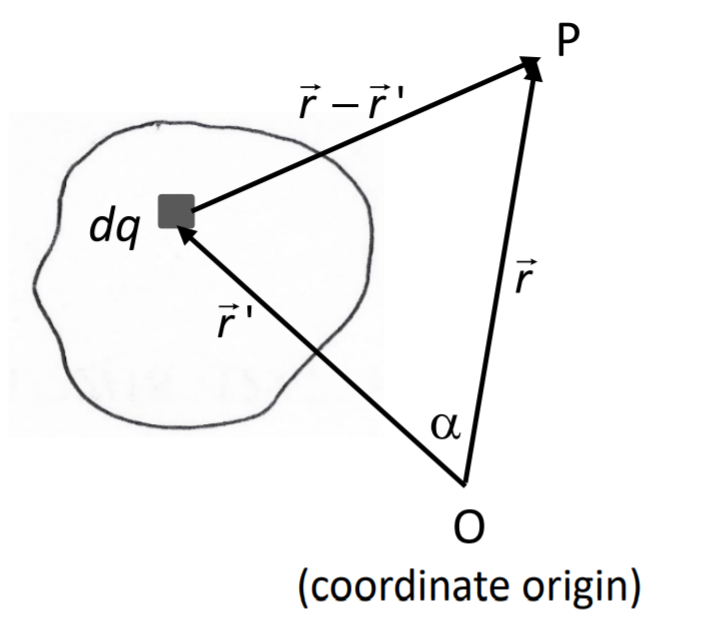
\includegraphics[scale=0.3]{multipoleExpansions.png}
\end{center}

The large distance behavior can be studied through expansion. The problem has two distance scales, $r$ and $r'$. Large distance here means $r>>r'$.
\begin{align*}
\frac{1}{\sqrt{r^2 + (r')^2 -2rr'\cos(\alpha)}} = \frac{1}{r}\frac{1}{\sqrt{1+(r'/r)^2 - 2(r'/r)\cos(\alpha)}} \tag{$\mathcal{R}$}
\end{align*}
Taylor expansion for $(\mathcal{R})$ about the variable $r'/r$ around $r'/r = 0$ is a power series with Legendre polynomials given by the following:
$$ (\mathcal{R}) = \frac{1}{r}\frac{1}{\sqrt{1+(r'/r)^2 - 2(r'/r)\cos(\alpha)}} = \frac{1}{r}\sum_{n=0}^\infty \left(\frac{r'}{r}\right)^nP_n(\cos(\alpha))$$
where we have:
$P_0(x) = 1 \qquad P_1(x) = x \qquad P_2(x) = \frac{3x^2-1}{2}\qquad P_3(x) = \frac{5x^3 - 3x}{2}\qquad \cdots$
Thus the potential $V(\vec{r})$ can be written as the following:
\begin{align*}
V(\vec{r}) 
&= \frac{1}{4\pi \epsilon_0}\, \sum_{n=0}^\infty \left(\frac{1}{r^{n+1}} \int (r')^nP_n(\cos(\alpha))\, dq\right)\\ 
&= \frac{1}{4\pi \epsilon_0}\left( \frac{1}{r}\left(\int\, dq\right) + \frac{1}{r^2}\left(\int r'\cos(\alpha)\,dq\right) + \frac{1}{r^3}\left(\int (r')^2\, \frac{3\cos^2(\alpha)-1}{2}\,dq\right)+\cdots\right) \tag{$\mathcal{T}$}
\end{align*}

At large distances, high-order terms become less important as $(r'/r)^n$ approaches zero. Depending on the precision needed, one can decide how many terms to use. 

The first term in equation ($\T$) is given by the following:
$$V_{mon}(\vec{r}) = \frac{1}{4\pi \epsilon_0}\frac{1}{r}\int \, dq = \frac{1}{4\pi \epsilon_0}\frac{Q}{r}$$
Here $V_{mon}$ is called the monopole term, to the $0$-th order. The charge distribution looks like a point charge for a point of interest far away if only $V_{mon}$ is included in the calculation.\\

The second term in ($\T$) is given by the following:
\begin{align*}
V_{dip}(\vec{r}) = \frac{1}{4\pi \epsilon_0}\frac{1}{r^2}\int r'\cos(\alpha)\, dq = \frac{1}{4\pi \epsilon_0}\frac{1}{r^2}\int(\hat{r}\cdot \vec{r}')\, dq = \frac{1}{4\pi \epsilon_0}\frac{\hat{r}}{r^2}\cdot \int \vec{r}'\, dq
\end{align*}
Here $V_{dip}$ is called the dipole term, to the first order. We also define $\vec{p} \coloneqq \int \vec{r}'\, dq$ to be the dipole moment. Hence we have:
$$V_{dip}(\vec{r}) = \frac{1}{4\pi \epsilon_0}\frac{\vec{p}\cdot \hat{r}}{r^2}$$
The third term, $n=2$, to the second order, in $(\T)$ is called the quadrupole term.\\
The fourth term, $n=3$, to the third order, in $(\T)$ is called the octupole term. 

\newpage
\subsection*{Multiple Expansion of a Point Charge}
Consider a point charge $q$ at the origin has a pure or ideal monopole potential given by:
\begin{align*}
V(\vec{r}) = V_{mon}(\vec{r}) = \frac{1}{4\pi \epsilon_0} \frac{q}{r}
\end{align*}
In this case, the potential has no high-order contribution, no dipole nor quadrupole. The total charge $q$ is also referred to a monopole.\\

A point charge $q$ placed at $\vec{r}'$ away from the origin will have high-order terms:
\begin{align*}
V(\vec{r}) = \frac{1}{4\pi \epsilon_0}\frac{q}{|\vec{r}-\vec{r}'|} = \frac{1}{4\pi \epsilon_0}\frac{q}{r} + \frac{1}{4\pi \epsilon_0}\frac{(q\vec{r}')\cdot \hat{r}}{r^2}+\cdots
\end{align*}
In such case, the potential has higher-order contributions, it has a dipole moment $\vec{p} = q\vec{r}'$.\\

\subsection*{Coordinate Origin in Multipole Expansion}
The examples in the multiple expansion of a point charge illustrate that the choice of coordinate origin is critical for multipole expansion.\\

The total charge $q$ is independent of the choice of the coordinate origin, but in general, the dipole and higher-order moments are dependent on the choice.\\

For example, if the coordinate origin is shifted by $\vec{a}$, the monopole and dopole moment are then given by:
\begin{align*}
\bar{q} = \int dq = q \qquad\qquad\qquad \vec{\bar{p}} = \int \vec{\bar{r}}'\,dq = \int(\vec{r}'-\vec{a})\,dq =\vec{p}-q\vec{a}
\end{align*}
Note that $\vec{\bar{p}} = \vec{p}$ if $q = 0$. Here $\vec{\bar{p}}, \vec{\bar{q}}$ denotes quantities calculated with the coordinate origin shifted, while $\vec{p},\vec{q}$ denote quantities without coordinate shifted.
\begin{center}
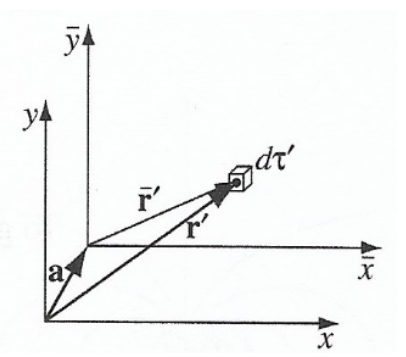
\includegraphics[scale=0.5]{multipoleOrigin.png}
\end{center}


\subsection*{Physical Electric Dipole}
\begin{defn}
Physical electric dipole consists of two equal and opposite charges $\pm q$ separated by a distance $d$. 
\end{defn}

The dipole moment of such physical dipole is given by the following:
\begin{align*}
\vec{p} = \int \vec{r}\, dq = \sum_i q_i \vec{r}_i = q\vec{r}_1 - q\vec{r}_2 = q\vec{d}
\end{align*}
where $\vec{r}_1,\vec{r}_2$ represents the position of the two charges and $\vec{d}$ satisfies $\vec{r}_2 + \vec{d} = \vec{r}_1$. Note here $\vec{d}$ is the vector from the position of the negative charge to the positive charge. $\vec{p}$ here does not depend on the choice of origin because total charge of the system is zero. The monopole contribution is also zero because the total charge of the system is also zero.\\

The potential of the physical electric dipole is dominated by the dipole term, but has higher-order contributions:
\begin{align*}
V(\vec{r}) = \frac{1}{4\pi \epsilon_0}\frac{\vec{p}\cdot \hat{r}}{r^2} + \cdots
\end{align*}
\newpage

\subsection*{Ideal or Pure Electric Dipole}
\begin{defn}
Ideal or pure electric dipole is an idealized physical dipole that satisfies:
Given $q$, $\vec{d}$, and $\vec{p}$ defined above, when $||\vec{d}||$ tends to zero, then $q$ tends to infinity, such that $||\vec{p}|| = q||\vec{d}||$ is finite. 
\end{defn}

An ideal dipole is a point object without physical size. If the ideal dipole is placed at the origin of a coordinate, its potential has only the dipole term given by the following:
\begin{align*}
V(\vec{r}) = \frac{1}{4\pi \epsilon_0}\frac{\vec{p}\cdot \hat{r}}{r^2}
\end{align*}
Note that it will still have higher-order terms if not placed at the coordinate origin.\\
\begin{center}
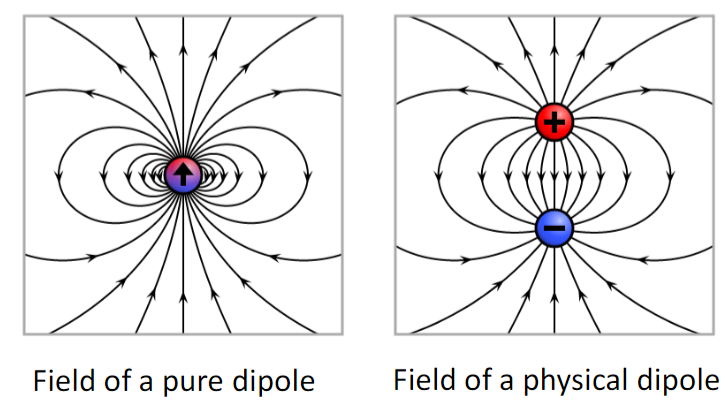
\includegraphics[scale=0.5]{dipole.png}
\end{center}

\subsection*{Electric Field of a Dipole}
A pure dipole placed at the origin with dipole moment $\vec{p}$ pointing in the $z$ direction has the potential given of the form:
\begin{align*}
V_{dip}(\vec{r}) = \frac{1}{4\pi \epsilon_0}\frac{\vec{p}\cdot \hat{r}}{r^2} = \frac{1}{4\pi \epsilon_0}\frac{||\vec{p}||\cos(\theta)}{r^2}
\end{align*}

The electric field of such ideal dipole is then given by $\vec{E} = -\nabla V_{dip}(\vec{r})$:
\begin{align*}
\vec{E}_{dip}(\vec{r}) = \frac{1}{4\pi \epsilon_0}\frac{1}{r^3}\left(3(\vec{p}\cdot \hat{r})\hat{r}-\vec{p}\right) \tag{ED}
\end{align*}
In spherical coordinates, equation (ED) can be written as the following:
\begin{align*}
\vec{E}_{dip}(\vec{r}) = \begin{bmatrix}
E_r & E_\theta & E_\phi
\end{bmatrix} &= \bmat{-\frac{\partial V_{dip}}{\partial r} & -\frac{1}{r}\frac{\partial V_{dip}}{\partial \theta} & \frac{1}{r\sin(\theta)}\frac{\partial V_{dip}}{\partial \phi}}
=\bmat{\frac{2p \cos(\theta)}{4\pi \epsilon_0 r^3} & \frac{p \sin(\theta)}{4\pi \epsilon_0 r^3} & 0}
\end{align*}
or equivalently, we can write:
\begin{align*}
\vec{E}_{dip}(\vec{r}) = \frac{1}{4\pi \epsilon_0}\frac{p}{r^3}(2\cos(\theta)\hat{r} + \sin(\theta) \hat{\theta})
\end{align*}
Note that we have the following relation:
\begin{align*}
E_{mon} \propto \frac{1}{r^2}\qquad\qquad\qquad\qquad E_{dip}\propto \frac{1}{r^3}
\end{align*}


\newpage
\chapter{Potentials}
In electrostatics, the primary is to find the electric field. For problems with conductors, the charge distribution may not be known since charge is free to move. Often only the total charge on a conductor is known. In any kinds of problem, if the charge distribution in space is known, one can find the electric field by Coulomb's law:
$$\vec{E}(\vec{r}) = \frac{1}{4\pi \epsilon_0} \int \rho(\vec{r}') \frac{\vec{r}- \vec{r}'}{||\vec{r}-\vec{r}'||^3}\, d\tau'$$

Unfortunately vector integrals are difficult to calculate except for a few special cases with symmetry for which Gauss's law applies. Fortunately, the scalar potential has all the information about the electric field. It can be found through integration given by:
\begin{align*}
V(\vec{r}) = \frac{1}{4\pi \epsilon_0}\int \frac{\rho (\vec{r}')}{||\vec{r}-\vec{r}'||}d\tau'
\end{align*}
It can also be stated in differential form with boundary conditions given in the problem, given by the Poisson's Equation along with the boundary conditions:
\begin{align*}
\nabla^2 V(\vec{r}) = -\frac{\rho(\vec{r})}{\epsilon_0}
\end{align*}
If there is no charge in the region of interest, Poisson's equation reduces to Laplace's equation:
\begin{align*}
\nabla^2 V(\vec{r}) = 0 \tag{LP}
\end{align*}
Equation (LP) is linear in the sense that any linear combination of the solutions is also a solution. If $V_1,\, V_2,\, V_3,\cdots$ are solutions to equation (LP), then $V=c_1V_1+c_2V_2+c_3V_3 +\cdots  = \sum_i c_iV_i$ is also a solution to equation (LP), with $c_i$ being arbitrary constant.\\

\section[Laplace's Equations and Poisson's Equations]{\color{red}Laplace's Equations and Poisson's Equations\color{black}}
When solving Lapalce's Equation or Poisson's Equation, which are second order differential equations, the solution is unique only when we make use of the boundary conditions. Hence one will need to boundary conditions given in the problem to find the scalar electric potential field in the region of interest. \\

\subsection*{Laplace's Equation in One Dimension}
Laplace's Equation in one dimension is of the form given by the following:
$$\frac{d^2 V}{dx^2} = 0 \qquad\qquad\qquad\text{with }  V:\R \to \R \ \ \ x\mapsto mx+b $$
The general solution is a straight line which has the following properties:
\begin{enumerate}
\item Given a point $x\in \R$, $V(x)$ is the average of the two symmetric neighboring points. For $a \in \R$, we have:
\begin{align*}
V(x) = \frac{1}{2}(V(x+a)+V(x-a))
\end{align*}
\item Maximum and minimum must occur at the end points, sine $V(x)$ is the average of its neighboring points, there does not exist any local maximum nor local minimum unless $V(x)$ is a constant function.
\end{enumerate}
\newpage

\subsection*{Laplace's Equation in Two Dimension}
Laplace equation in two dimension is of the form given by the following:
\begin{align*}
\left(\frac{\partial^2}{\partial x^2}+\frac{\partial^2}{\partial y^2}\right)V = 0 \qquad\qquad\qquad\qquad \text{with }V:\R^2 \to \R
\end{align*}
There is no simple generation solution for such equation. Nevertheless, the solution $V$ can be shown to satisfy the following properties:
\begin{enumerate}
\item Given a point $(x,y) \in \R^2$, $V(x,y)$ is an average of its neighboring points. That is, for any $R>0$, let $P$ be a circular path of radius $R$ centered at $(x,y)$, we have the following holds:
\begin{align*}
V(x,y) = \frac{1}{2\pi R}\int_P V\, dl
\end{align*}
\item All maxima and minima occur at the boundaries of the surface of interest. 
\end{enumerate}

\subsection*{Laplace's Equation in Three Dimensions}
Laplace's Equation in three diensions is of the form given by the following;
\begin{align*}
\left(\frac{\partial^2}{\partial x^2}+\frac{\partial^2}{\partial y^2}+\frac{\partial^2}{\partial z^2}\right)V = 0 \qquad\qquad\qquad\qquad \text{with }V:\R^3 \to \R
\end{align*}
The properties are similar:
\begin{enumerate}
\item Given a point $\vec{r}\in \R^3$, $V(\vec{r})$ is the average value of $V$ over a spherical surface $S$ of radius $R$ centered at $\vec{r}$ for arbitrary positive $R$:
\begin{align*}
V(\vec{r}) = \frac{1}{4\pi R^2}\oint_{S} V\, da
\end{align*}
\item All maxima and minima occur at the boundaries of the closed surface of interest. $V$ has no local extrema. 
\end{enumerate}

\note In layman's language, solutions to the Laplace's equation are smoothly increasing or decreasing functions, there is no bump nor crater in the middle.\\

\subsection*{Boundary Conditions}
Solving Laplace's equation is a critical step to determine $V$. However, Laplace's equation alone
does not unique determine a solution $V$. Taking one-dimensional case, the solution is given by:
$$V(x) = mx+b$$
However, there are two arbitrary constants, $m$ and $b$, from the integration. Additional information such as boundary conditions are needed, which could be the values of $V$ or $\frac{dV}{dx}$ at the end points.\\

In two or three dimensions, Laplace's Equation is of the form in partial differential equations, the boundaries are closed loops in two dimensions or closed surfaces in three dimensions. In this case, it is not obvious what kind boundary conditions are needed to uniquely determine the potential.
Sets of boundary conditions which are sufficient to uniquely determine the potential are
summarized in a number of uniqueness theorem.\\


\begin{thm}[First Uniqueness Theorem]
The solution to Laplace's equation in a region is uniquely determined if $V$ is specified on all its boundary surfaces. 
\end{thm}

\begin{center}
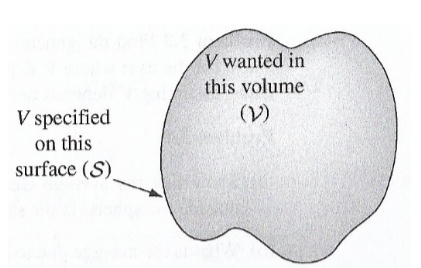
\includegraphics[scale=0.5]{uniqueThm1.png}
\end{center}

When applying the first uniqueness theorem, note that Laplace's Equation implies no charge inside the region of interest. The region of interest could have holes, but we can still apply first uniqueness theorem as long as $V$ is specified on the surface of the hole as well. The region could also extend to infinity at which $V$ is usually assumed to be zero. 

\begin{proof}[Proof of the First Uniqueness Theorem]
Suppose there are two solutions $V_1$ and $V_2$ to a Laplace's equation with the same values on the boundary surfaces of interest. Note that $V_3= V_2 - V_1$ is also a solution to the problem. Since $V_1$ and $V_2$ have the same values on the boundary surfaces of interest, $V_3$ should be zero on all boundary surfaces of interest. Note that for all solutions to the Laplace's equation, extrema occur on the boundaries. Since the maximum and minimum of $V_3$ are both zero, $V_3$ must be zero everywhere in the region of interest. Therefore we can conclude that $V_1 = V_2$. 
\end{proof}

Here we see that, whetever the solution we get that meets the boundary conditions, that must be the right solution.\\

\begin{corT}[First Uniqueness Theorem in a Region with Charge]
The potential in a region is uniquely determined if both the charge density throughout the region and the value of $V$ on all boundaries are specified. 
\end{corT}

\begin{proof}
Suppose there are two solutions $V_1$ and $V_2$ to a Poisson's equation $\nabla^2 V = -\rho /\epsilon_0$ with the same values on the boundary surfaces of interest. Note that $V_3= V_2 - V_1$ is a solution to the Laplace equation $\nabla^2 V_3 = \nabla^2 V_2 - \nabla^2 V_1 = 0$. Since $V_1$ and $V_2$ have the same values on the boundary surfaces of interest, $V_3$ should be zero on all boundary surfaces of interest. Note that for all solutions to the Laplace's equation, extrema occur on the boundaries. Since the maximum and minimum of $V_3$ are both zero, $V_3$ must be zero everywhere in the region of interest. Therefore we can conclude that $V_1 = V_2$. 
\end{proof}

In mathematics, there are two common boundary conditions for differential equations:
\begin{enumerate}[topsep=3pt,itemsep=-1ex,partopsep=1ex,parsep=1ex]
\item Dirchlet. The values of the solution on the boundaries are known.
\item Neumann. The values of the normal derivative of the solution on the boundaries are known.
\end{enumerate}
Both conditions are sufficient to uniquely define the potential. However, the Neumann condition allows for an overall unimportant constant. \\


\begin{thm}[Second Uniqueness Theorem]
In a region surrounded by conductors and with known charge density $\rho$. The electric field is uniquely determined if the total charge on each conductor is given. Note that the region as a whole can be bounded by another conductor.
\end{thm}
\begin{center}
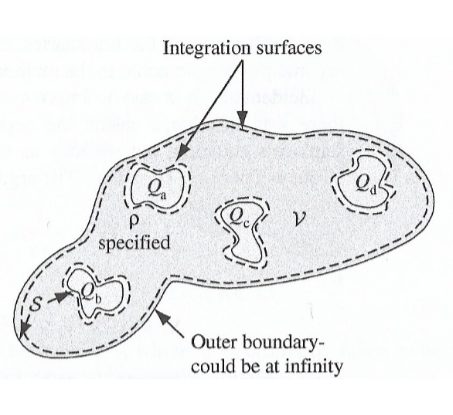
\includegraphics[scale=0.5]{uniqueThm2.png}
\end{center}
\begin{proof}[Proof of the Second Uniqueness Theorem]
Suppose there are two fields, both obey Gauss's Law in the region of interest, that is, we can write:
$$\nabla \cdot \vec{E}_1=\nabla \cdot \vec{E}_2 = \frac{\rho}{\epsilon_0}$$
and they satisfy the integral form of Gauss's Law on the boundaries, that is, we can write:
\begin{align*}
\oint_S \vec{E} _1 \cdot d\vec{a} = \oint_S \vec{E}_2 \cdot d\vec{a} &= \frac{Q_{total}}{\epsilon_0}\qquad\qquad \text{for outer boundary } S \\
\oint_{S_i} \vec{E} _1 \cdot d\vec{a} = \oint_{S_i} \vec{E}_2 \cdot d\vec{a} &= \frac{Q_i}{\epsilon_0}\qquad\qquad\quad\ \text{for the boundary of the i-th conductor } S_i
\end{align*}
Then the difference between the two fields $\vec{E}_3 \coloneqq \vec{E}_1 - \vec{E}_2$ satisfies $\nabla \vec{E}_3 = 0$ in the region and $\oint \vec{E}_3 \cdot d\vec{a} = 0$ on all surfaces $S$ and $S_i$. Let $V_3$ be the potential for $\vec{E}_3$, that is, $\vec{E}_3 = -\nabla V_3$. Since each conductor is an equipotential, then $V_3$ must be zero over each conducting surface. Thus we can write the following:
\begin{align*}
\int (E_3)^2\, d\tau 
&= \int \vec{E}_3 \cdot \vec{E}_3 \, d\tau \\
&= -\int \vec{E}_3 \cdot \nabla V_3\, d\tau \\
&= -\int\left(\nabla \cdot (V_3\vec{E}_3) - V_3(\nabla \cdot \vec{E}_3)\right)\, d\tau \\
&=-\oint V_3 \vec{E}_3 \cdot d\vec{a} \\
&= -V_3\oint \vec{E}_3\cdot d\vec{a} = 0
\end{align*}
Since the integrand $(E_3)^2$ is always non-negative, then we must have $\vec{E}_3 = 0$, hence we have $\vec{E}_1 = \vec{E}_2$. This completes the proof of this theorem.
\end{proof}

The uniqueness theorems are licenses for hunting for solution of a given Laplace's Equation or Poisson's Equation along with the boundary conditions in the region of interest. The solutions one can find must be the correct ones if they meet the boundary conditions.\\

\begin{thm}[Earnshaw's Theorem]
A charged particle cannot be held in a stable equilibrium by electrostatic forces only. 
\end{thm}
\begin{center}
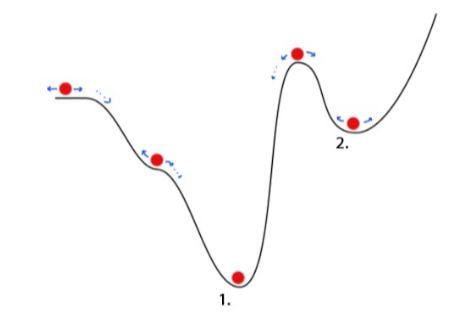
\includegraphics[scale=0.5]{earnshaw.png}
\end{center}

Stable equilibrium corresponds to local minimum in potential energy, but the electrostatic potential has no local extrema. Hence a charged particle cannot be held in a stable equilibrium by electrostatic forces only. \\

Note that there is only one way to distribute the charge on a conductor if everything else is the same according to the second uniqueness theorem. \\
\begin{center}
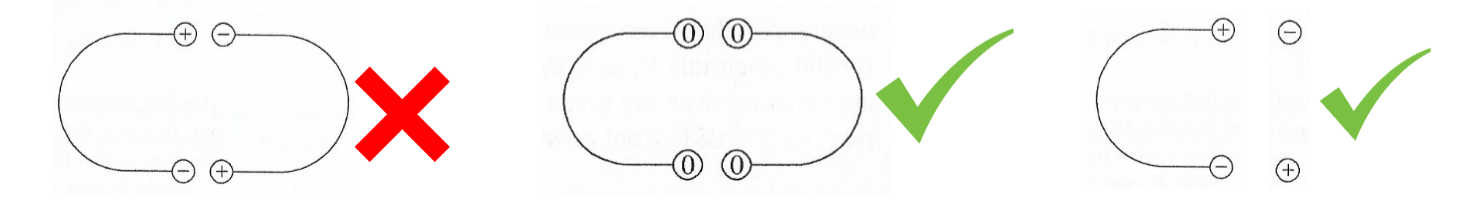
\includegraphics[scale=0.35]{thmNotes.png}
\end{center}

\newpage
\section[Method of Images]{\color{red}Method of Images\color{black}}
The method of image is only applicable to very special cases, such as conducting planes, conducting spheres, conducing cylinders, point charges, line charges, and so on. In such method, we note that the image charge must be placed outside the region of interest. The image charge has opposite sign as the original charge. The total induced charge is equal to the image charge. \\


The following will discuss two classic examples:

\begin{center}
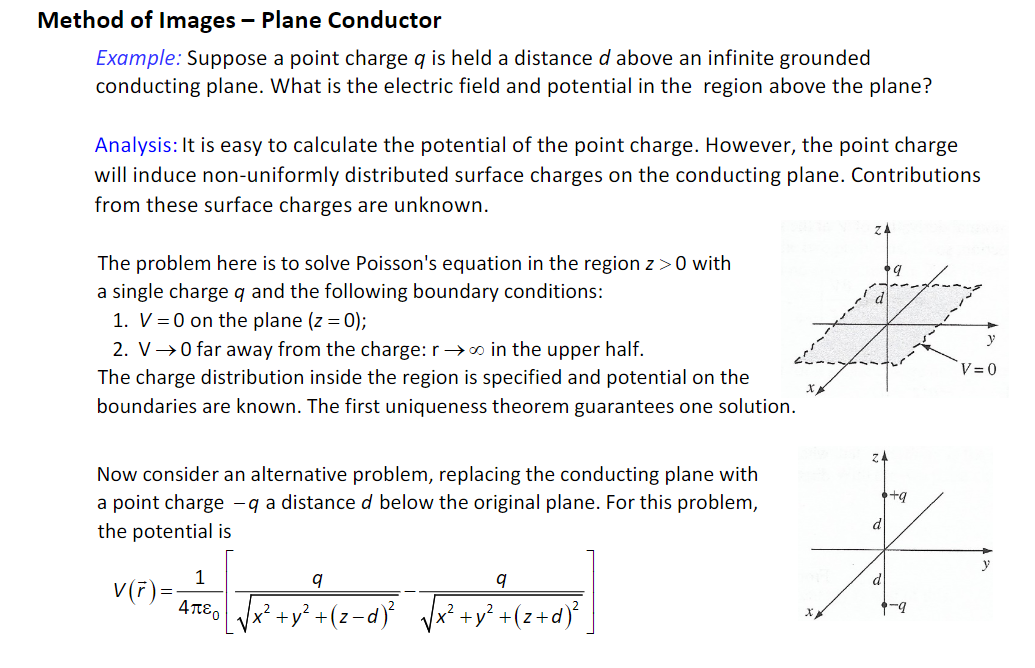
\includegraphics[scale=0.5]{imageMthd1.png}
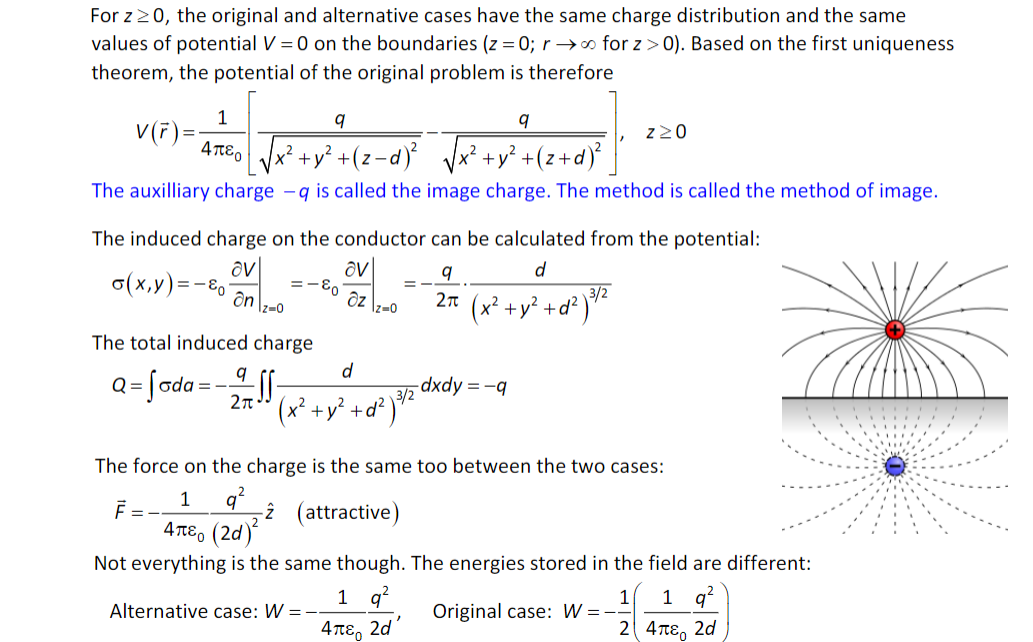
\includegraphics[scale=0.5]{imageMthd2.png}
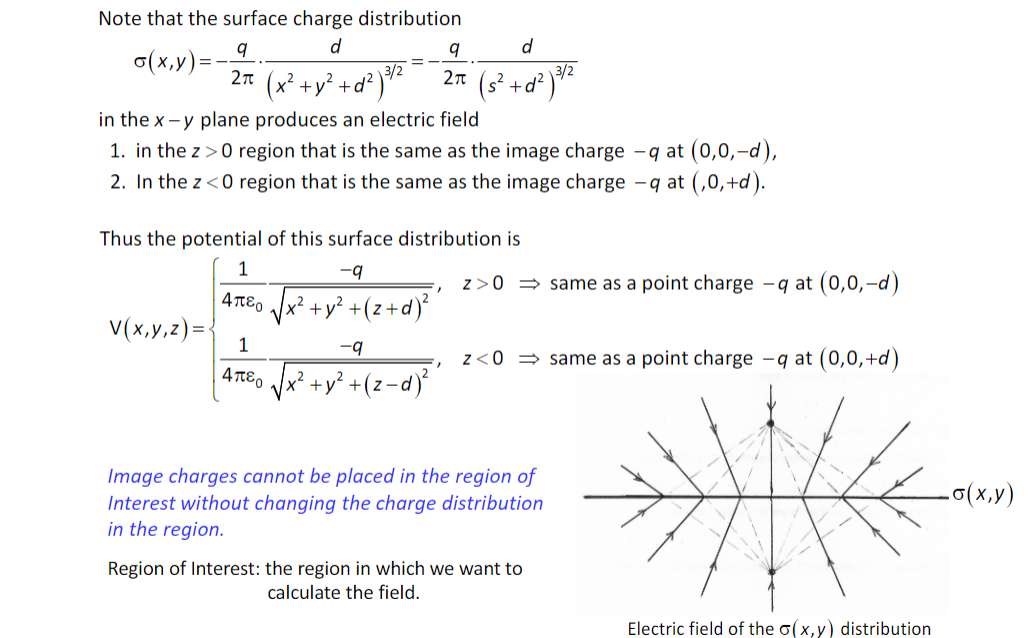
\includegraphics[scale=0.5]{imageMthd3.png}
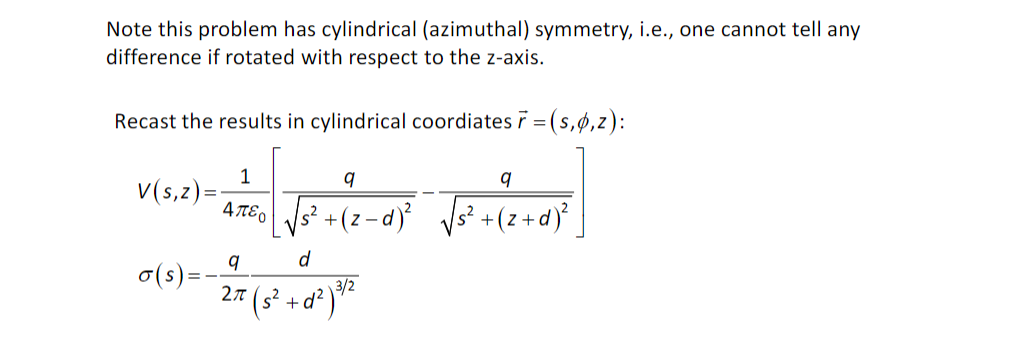
\includegraphics[scale=0.5]{imageMthd4.png}\\
\hfill\break
\hfill\break
\hfill\break
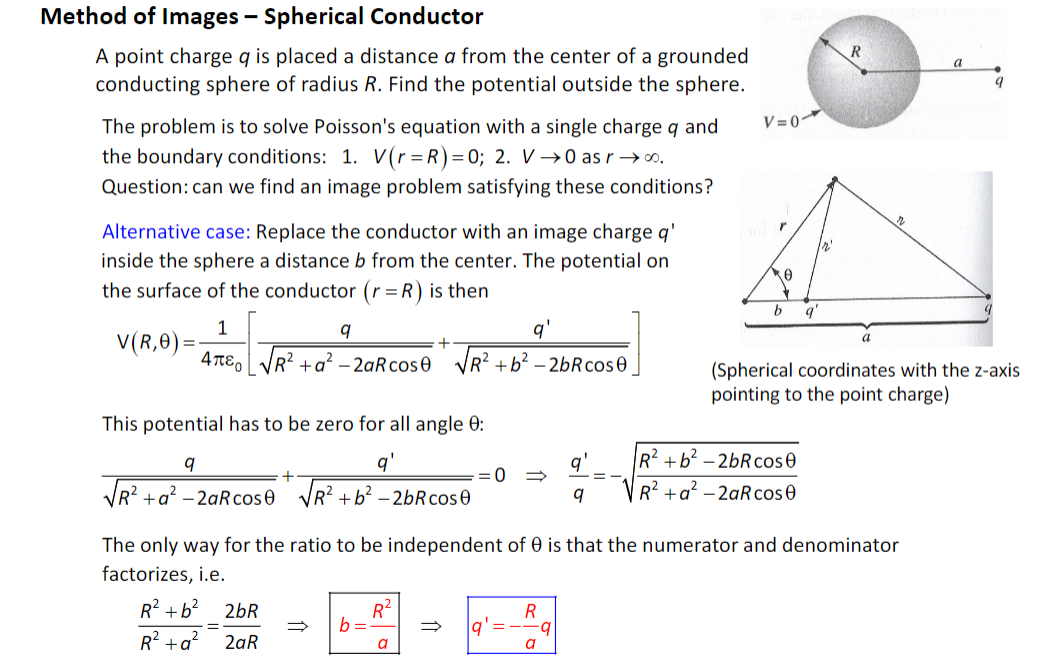
\includegraphics[scale=0.5]{imageMthd5.png}
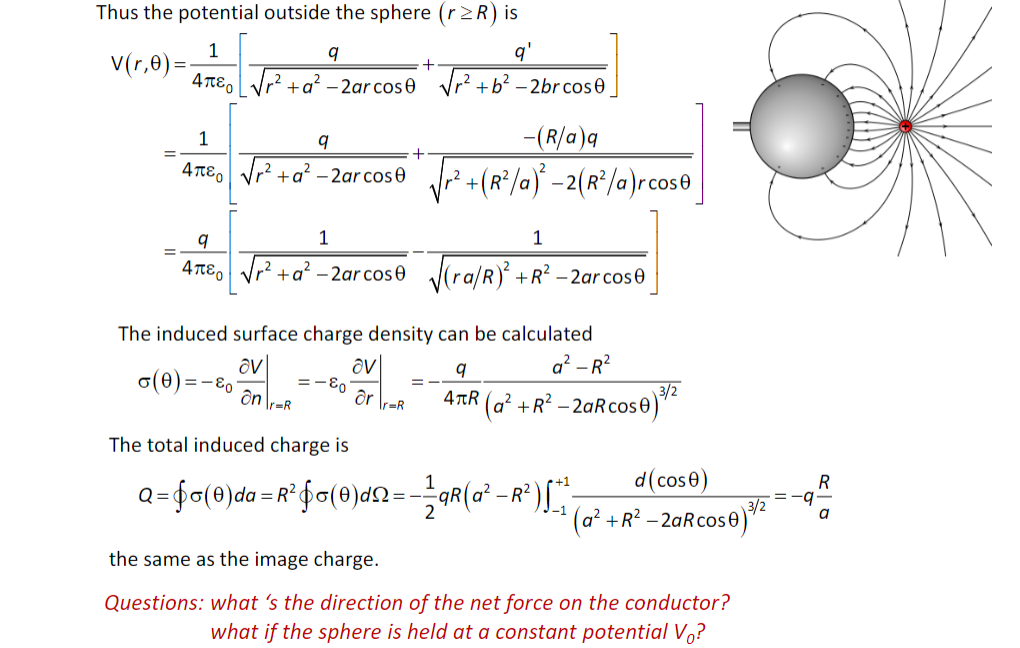
\includegraphics[scale=0.5]{imageMthd6.png}
\end{center}



\newpage
\section[Differential Equations and Boundary Problems]{\color{red} Differential Equations and Boundary Problems\color{black}}
One of the most important methods for solving partial differential equations is
the separation of variables. It looks for solutions that are product of functions, each depends on only one of the coordinates. Illustrating the method in Cartesian coordinates.\\

\example\\
Two infinite grounded metal plates parallel to the $xz$-plane, one at $y=0$ and the other at $y=a$. The left end, at $x=0$, is 
closed off with an infinite strip insulated from the two plates and maintained a potential $V_0(y)$. Find the potential in between the two plates.\\

\begin{center}
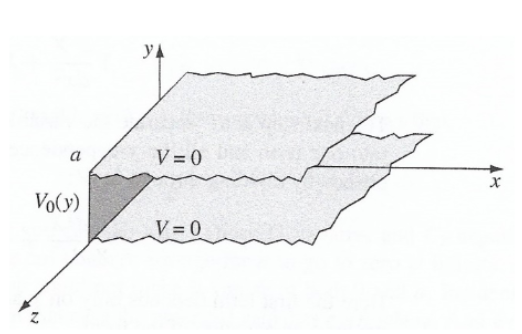
\includegraphics[scale=0.5]{pde1.png}
\end{center}

The problem is to solve Laplace's Equation subject to the boundary conditions:
\begin{enumerate}[topsep=3pt,itemsep=-1ex,partopsep=1ex,parsep=1ex]
\item $V=0$ at $y=0$
\item $V=0$ at $y=a$
\item $V=V_0(y)$ at $x=0$\\
\item $V$ approaches $0$ as $x$ approaches infinity
\end{enumerate}

The configuration is $z$-independent, we look for solutions in two dimensions, hence we can write:
\begin{align*}
\left(\frac{\partial^2}{\partial x^2}+\frac{\partial^2}{\partial y^2}\right) V(x,y) = 0 \tag{P}
\end{align*}
The method of separation of variables starts with solutions of the form:
\begin{align*}
V(x,y) = X(x)\cdot Y(y) \tag{S}
\end{align*}
that the product of two functions $X(x)$ and $Y(y)$ gives a solution to PDE (P). $X(x)$ only depends on variable $x$, and $Y(y)$ only depends on variable $y$.\\

With (S), one can rewrite (P) as the following:
\begin{align*}
\frac{1}{X}\frac{d^2X}{dx^2} + \frac{1}{Y}\frac{d^2Y}{dy^2} = 0 \tag{P'}
\end{align*}
The first term depends on $x$ only and the second term depends on $y$ only. (P') is possible only if each is a constant since $x$ and $y$ are independent variables. That is, we can write the following:
\begin{align*}
\frac{d^2X}{dx^2} = X\,k^2 \qquad\qquad\qquad \frac{d^2 Y}{dy^2} = -Y\,k^2 \tag{O}
\end{align*}
The PDE (P') becomes two ODEs. The solutions for the two ODEs are given by the following:
\begin{align*}
X(x) = Ae^{kx}+Be^{-kx}\qquad\qquad\qquad Y(x) = C\sin(ky)+D\cos(ky)
\end{align*}
with $A,B,C,D$ being constants determined by the boundary conditions. Here we get:
\begin{align*}
V(x,y) = (Ae^{kx} + Be^{-kx}) (C\sin(ky) + D\cos(ky))
\end{align*}
Boundary condition (4) requires $A = 0$, boundary condition (1) requires $D=0$, boundary condition (2) requires $k = \frac{n\pi }{a}$ with $n \in \N$. The constant $B$ is absorbed into $C$ and $D$. Hence the following solutions meet three out of four boundary conditions:
\begin{align*}
V_n(x,y) = Ce^{-n\pi x/a}\sin\left(\frac{n\pi}{a}y \right) \qquad\qquad n\in \N
\end{align*}
The boundary condition (3) is impossible to meet unless $V_0(y) \approx \sin(n\pi y/a)$. But we have derived an infinite set of solutions. The extraordinary properties of these solutions make it possible to construct a solution that meets the boundary condition.\\

The set of separable solutions $\{V_n \mid n\in \N\}$ are orthogonal and complete, any other function over the rage can be decomposed, hence we can construct a more general solution:
\begin{align*}
V(x,y) = \sum_{n=1}^\infty C_n e^{-n\pi x/a} \sin\left(\frac{n\pi y}{a}\right) 
\end{align*}
where boundary condition (3) is satisfied by setting the coefficient $C_n$ by the following:
\begin{align*}
C_n = \frac{2}{a}\int_0^a V_0(y)  \sin\left(\frac{n\pi y}{a} \right)\, dy \qquad \Rightarrow\qquad V(0,y) = \sum_{n=1}^\infty C_n  \sin\left(\frac{n\pi y}{a} \right) = V_0(y)
\end{align*}
If $V_0(y) = V_0$, then we get the following:
\begin{align*}
C_n =\frac{2}{a}\int_0^a V_0 \sin\left(\frac{n\pi y}{a} \right)\, dy = \begin{cases}0 & n \text{ is even}\\ \frac{4V_0}{n\pi} & n \text{ is odd}    \end{cases} 
\end{align*}
Thus we can write the solution:
\begin{align*}
V(x,y) = \frac{4V_0}{\pi}\sum_{n \text{ is odd}} \frac{1}{n} e^{-n\pi x/a} \sin\left(\frac{n\pi y}{a} \right)  
\end{align*}
\hfill\break
\hfill\break
\hfill\break
\example\\
An infinitely long rectangular metal pipe is grounded, bounded by $xz$-plane, $xy$-plane, $zy$-plane, $z=b$ plane, and $y=a$ plane. But one end at $x=0$ is maintained at a specified potential $V_0(y,z)$. Find the potential inside the pipe. 
\begin{center}
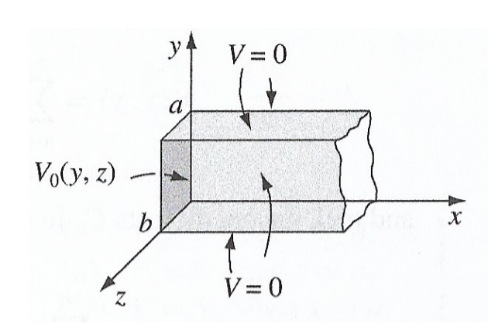
\includegraphics[scale=0.5]{pde2.png}
\end{center}
This is a three-dimensional Laplace's equation problem, we set up a PDE:
\begin{align*}
\left( \frac{\partial^2}{\partial^2 x}+\frac{\partial^2}{\partial^2 y} + \frac{\partial^2}{\partial^2 z}\right)V(x,y,z) = 0
\end{align*}
with the boundary conditions:
\begin{enumerate}[topsep=3pt,itemsep=-1ex,partopsep=1ex,parsep=1ex]
\item $V=0$ at $y=0$
\item $V=0$ at $y=a$
\item $V=0$ at $z=0$
\item $V=0$ at $z=b$
\item $V$ approaches $0$ as $x$ approaches $\infty$
\item $V=V_0(y,z)$ at $x=0$
\end{enumerate}

Solve the PDE with initial conditions through the method of separation of variables, we get the following solution:
\begin{align*}
V(x,y,z) = \sum_{m=1}^\infty \sum_{n=1}^\infty C_{mn}e^{-\sqrt{(m/a)^2 + (n/b)^2}\pi x}\sin\left(\frac{m\pi y}{a}\right)\sin\left( \frac{n\pi z}{b}\right)
\end{align*}
with $m,n \in \N$, we $C_{mn}$ is given by the following:
\begin{align*}
C_{mn} = \frac{4}{ab}\int_0^b \int_0^a V_0(y,z)\sin\left(\frac{m\pi y}{a}\right)\sin\left( \frac{n\pi z}{b}\right)\, dy\, dz 
\end{align*}

\newpage
\subsection*{Separation of Variables in Spherical Coordinate}
In spherical coordinate, the Laplace's Equation has the following form:
\begin{align*}
\nabla^2 V = \frac{1}{r^2}\frac{\partial}{\partial r}\left( r^2 \frac{\partial V}{\partial r}\right) + \frac{1}{r^2\sin(\theta)}\frac{\partial}{\partial \theta}\left( \sin(\theta) \frac{\partial V}{\partial \theta}\right) + \frac{1}{r^2 \sin^2(\theta)}\frac{\partial^2 V}{\partial \phi^2} = 0
\end{align*}
For simplicity, we will only deal with azimuthal symmetry, that is, we suppose $V = V(r,\theta)$, then we get:
\begin{align*}
\frac{1}{r^2}\frac{\partial}{\partial r}\left( r^2 \frac{\partial V}{\partial r}\right) + \frac{1}{r^2\sin(\theta)}\frac{\partial}{\partial \theta}\left( \sin(\theta) \frac{\partial V}{\partial \theta}\right)  = 0 \tag{PS}
\end{align*}
Separation of variables suggests that a solution to the PDE (PS) is given of the form:
\begin{align*}
V(r,\theta) = R(r) \cdot \Theta(\theta) \tag{SS}
\end{align*}
Combining equation (SS) and PDE (PS) we get the following:
\begin{align*}
\frac{1}{R}\frac{d}{dr}\left( r^2 \frac{dR}{dr}\right) + \frac{1}{\Theta\sin(\theta)}\frac{d}{d\theta}\left( \sin(\theta) \frac{d\Theta}{d\theta}\right) = 0
\end{align*}
Since the first term depends only on $r$ and the second term depends only on $\theta$, there must exists $l\in \N\cup\{0\}$ such that the following holds:
\begin{align*}
\frac{1}{R}\frac{d}{dr}\left( r^2 \frac{dR}{dr}\right) = l(l+1) \qquad\qquad \qquad \qquad \frac{1}{\Theta\sin(\theta)}\frac{d}{d\theta}\left( \sin(\theta) \frac{d\Theta}{d\theta}\right) = -l(l+1)
\end{align*}
The choice of the separation constant $l(l+1)$ might seem strange at this step, but the reason will be apparent later. The radial equation has the solution of the form given by:
\begin{align*}
\frac{d}{dr}\left( r^2 \frac{dR}{dr}\right) = l(l+1)R \qquad \qquad \Rightarrow \qquad R_l(r) = Ar^l +\frac{B}{r^{l+1}}
\end{align*}
where $A$ and $B$ are constants determined by the boundary conditions.\\

The angular equation given by:
\begin{align*}
\frac{d}{d\theta}\left(\sin(\theta)\, \frac{d\Theta}{d\theta}\right) = -l(l+1) \sin(\theta)\, \Theta
\end{align*}
for $l\in \N \cup\{0\}$, the angular equation ODE is the angular form of the Legendre differential equation. It becomes the familiar form with the change of variable $x = \cos(\theta)$.\\

One of the two independent complement solutions is the Legendre polynomials $P_l(\cos(\theta))$ given by the following:
\begin{align*}
\Theta_l(\theta) = P_l(\cos(\theta))
\end{align*} 
where the polynomials are given by the Rodrigues Formula with $x = \cos(\theta)$:
\begin{align*}
P_l(x) = \frac{1}{2^l l!}\left(\frac{d^l}{dx^l} (x^2-1)^l \right) \qquad \text{with }|x|\leq 1
\end{align*}
As a second-order ODE, the angular differential equation has a second independent solution for every $l$. Those solutions have singularities at $\theta = 0,\pi$, and are discarded on physical ground.\\

We conclude that the general solution of Laplace's Equation in spherical coordinates with $\phi$-symmetry is given by the following:
\begin{align*}
V(r,\theta) = \sum_{l=0}^\infty \left(A_l r^l +\frac{B_l}{r^{l+1}} \right)P_l (\cos(\theta))
\end{align*}
where $A_l$ and $B_l$ are determined by the boundary conditions. Note that for problems with $\phi$-symmetry, the angular solutions are spherical harmonics.\\



\newpage
\subsection*{Laplace's Equation in Cylindrical Coordinates}
Assuming that there is no $z$-dependence, the Laplace's equation in cylindrical coordinates has the form given by the following:
\begin{align*}
\nabla^2 V = \frac{1}{s}\frac{\partial}{\partial s}\left( s \frac{\pd V}{\pd S}\right) + \frac{1}{s^2} \frac{\pd^2 V}{\pd \phi^2} = 0 \tag{CP}
\end{align*}
One can try the solution $V(s,\phi) = S(s) \cdot \Phi (\phi)$ and combining with (CP) we get the following:
\begin{align*}
\frac{s}{S}\frac{d}{ds}\left( s\frac{dS}{ds}\right) + \frac{1}{\Phi}\frac{d^2 \Phi}{d\phi^2} = 0 \qquad\qquad \Rightarrow \qquad\qquad \frac{s}{S}\frac{d}{ds}\left( s \frac{dS}{ds}\right)  = n^2 = - \frac{1}{\Phi}\frac{d^2 \Phi}{d\phi}
\end{align*}
Here we see that $\Phi(\phi)$ must be oscillationary.\\

The solution to the azimuthal equation is of the form given by the following:
\begin{align*}
\Phi_n(\phi) = c_n \sin(n\phi) + d_n \cos(n\phi)
\end{align*}  
with $n \in \N \cup \{0\}$.\\

On the other hand, the solution to the radial equation is given by the following:
\begin{align*}
S_n(s) = a_n s^n + \frac{b_n}{s^n}
\end{align*}
with $n \in \N \cup \{0\}$.\\

The case of $n=0$ requires special care, we have $\Phi$ and $S$ being constants, so we have efectively found one solution for each of these second order differential equations:
\begin{align*}
\frac{d^2 \Phi}{d^2 \phi^2} = 0\qquad\qquad\qquad\qquad \qquad \frac{d}{ds}\left(s \frac{dS}{ds}\right) = 0 \tag{SO}
\end{align*}
It is clear that the solutions of these two equations (SO) are given by:
\begin{align*}
\Phi = c\phi +d \qquad\qquad\qquad \qquad \qquad S = a+b\ln(s) 
\end{align*}
since we have $\Phi$ is oscillatory, then we must have $c = 0$. \\

Combining the pieces together, we get the general solution for Laplace's equation in cylindrical coordinates:
\begin{align*}
V(s,\phi) = a_0 + b_0 \ln (s) + \sum_{n=1}^\infty \left( a_n s^n + \frac{b_n}{s^n}\right) (c_n \sin(n\phi) + d_n \cos(n\phi))
\end{align*}
The coefficients $a_i, b_i, c_i, d_i$ are determined by boundary conditions. Note that the set:
\begin{align*}
\{ 1,\ \sin(n\phi),\ \cos(n\phi) \mid n \in \N\}
\end{align*}
forms an orthogonal and complete set over the range $[0,2\pi]$. That is, we can write the following:
\begin{align*}
\int_0^{2\pi}\sin(m\phi)\sin(n\phi) \, d\phi = \pi \delta_{mn}\qquad \int_0^{2\pi}\cos(m\phi)\cos(n\phi) \, d\phi = \pi \delta_{mn} \qquad \int_0^{2\pi}\sin(m\phi)\cos(n\phi) \, d\phi = 0
\end{align*}

\newpage
\chapter{Electric Field in Matters}

In electrostatics, insulators are called dielectrics. Unlike conductors, all electrons in dielectrics are bound, that is, attached to their atoms, and therefore there are no free charges to move around inside the material. However, atoms or molecules do have charge distributions which can be affected by an external electric field. These microscopic changes are miniscule, but their cumulative effects give rise to the effects of dielectric materials in external electric field.\\

\section[Induced Electric Dipole]{\color{red}Induced Electric Dipole\color{black}}
An isotropic neutral atom has no intrinsic dipole moment, as positive and negative charge centers are at the same place. However, an external electric field will pull the two charge distributions in the opposite direction, leading to a slight shift between the positive 
and negative charge centers. Consequently, resulting a tiny dipole moment, called the induced dipole. The atom is said to be polarized.
\begin{center}
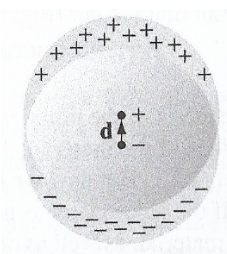
\includegraphics[scale=0.5]{PolarizedE.png}
\end{center}

For most materials, the dipole moment for each isotropic molecule is given by $\vec{p} = \alpha \vec{E}$ with some constant $\alpha$, as long as the field is not too strong. The constant $\alpha$ is a material property called the polarizability, typically $\alpha$ is of order $(4\pi \epsilon_0)\cdot 10^{-30}\, m^3$. For non-isotropic molecules, the induced dipole moment may depend on the $\vec{E}$ direction. For example, for $CO_2$ molecule, $\vec{p} = \alpha_\perp \vec{E}_\perp + \alpha_\parallel \vec{E}_\parallel$, where $\alpha_\perp$ and $\alpha_\parallel$ are different, and $\vec{E}_\perp$ and $\vec{E}_\parallel$ are the components of the electric field. In such case, we note that $\vec{p}$ and $\vec{E}$ might not be in the same direction.\\


For a completely asymmetric molecule, $\vec{p}=(p_x,p_y,p_z)$ and $\vec{E}=(E_x,E_y,E_z)$ have linear relation:
\begin{align*}
\bmat{p_x \\ p_y \\ p_z} = \bmat{\alpha_{xx} & \alpha_{xy} & \alpha_{xz} \\ \alpha_{yx} & \alpha_{yy} & \alpha_{yz} \\ \alpha_{zx} & \alpha_{zy} & \alpha_{zz}} = \bmat{E_x \\ E_y \\ E_z}
\end{align*} 
here the $\alpha$-matrix is called the polarization tensor.

\subsection*{A Primitive Model of Polarizability}
An atom consists of a point nucleus with charge $+q$ surrounded by a uniformly spherical cloud of negative charge $–q$ and radius $a$. One can find the polarizability.

\begin{center}
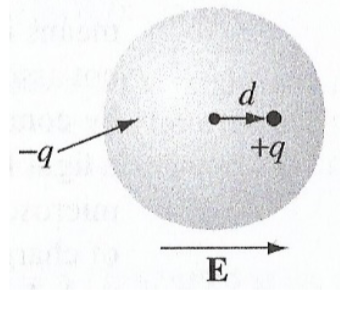
\includegraphics[scale=0.48]{PolarizedE1.png}
\end{center}

The positive charge, or the center of the negative charges cloud, is shifted a distance $d$ due to the external electric field. The positive charge $q$ is at an equilibrium of the two forces, (1) the force due to the external field, and (2) the force from the field of the negative charge cloud. \\

The electric field inside a uniformly charged sphere with total charge $-q$ is given by:
\begin{align*}
\vec{E}_{cloud}(\vec{r}) = \frac{-q}{4\pi \epsilon_0}\frac{\vec{r}}{a^3}
\end{align*}
The balance of the two forces requires the electric field produced by the cloud at $d$ away from the center of the cloud given by:
$$|E| = |E_{cloud}(\vec{d})| = \frac{q}{4\pi \epsilon_0}\frac{d}{a^3}$$
which requires:
$$p = qd = (4\pi \epsilon_0 a^3) E$$
thus the atomic polarizability is given by $\alpha = 4\pi \epsilon_0 a^3$. \\

Some molecules have intrinsic dipole moment, such as the $H_2O$ molecule. These molecules are called polar molecules. \\

These tiny dipoles are usually random oriented. However, in an external electric field, they will align in the direction of the field.\\

\subsection*{Electric Dipole in Electric Field}
In an uniform electric field, the dipole will experience a torque:
\begin{align*}
\vec{N} = \vec{r}_+ \times \vec{F}_+ + \vec{r}_- \times \vec{F}_- = \left(\frac{\vec{d}}{2} \right)\times (q\vec{E})+ \left(-\frac{\vec{d}}{2} \right)\times (-q\vec{E}) = (q\vec{d})\times \vec{E} = \vec{p}\times \vec{E}
\end{align*}
The effect of this torque is rotating $\vec{p}$ in the direction of $\vec{E}$.

\begin{center}
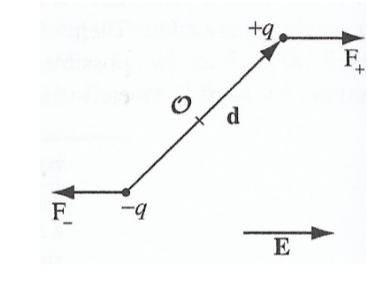
\includegraphics[scale=0.5]{torqueDipole.png}
\end{center}

Note that the total force on the dipole is zero in a uniform field, but this is not true for a non-uniform field:
\begin{align*}
\vec{F}_{net} = \vec{F}_+ + \vec{F}_- = q(\vec{E}_+ - \vec{E}_- ) = q\Delta \vec{E}
\end{align*}
where $\Delta \vec{E}$ represents the difference between the field at the two ends. Assuming that the dipole is short enough, then we can approximate the small change in the $x$-component of $E_x$ in the direction of $\vec{d}$, given by $\Delta E_x = (\nabla E_x) \cdot \vec{d}$, and hence with corresponding relation for $E_y$ and $E_z$, we can write:
\begin{align*}
\Delta \vec{E} = (\vec{d}\cdot \nabla) \vec{E}
\end{align*}
Combining we get:
\begin{align*}
\vec{F} = (\vec{p}\cdot \nabla) \vec{E}
\end{align*}
which gives a force experienced by a dipole $\vec{p}$ in a nonuniform field electric field $\vec{E}$.\\

The potential energy of a dipole in the field is given by:
\begin{align*}
U = qV_+ + (-q)V_- = q\Delta V = q(\nabla V \cdot \vec{d}) = -\vec{p}\cdot \vec{E}
\end{align*}

\subsection*{Dipole-Dipole Interaction}
From the electric field at $\vec{r}$ due to a dipole $\vec{p}$ at the origin:
\begin{align*}
\vec{E}(\vec{r}) = \frac{1}{4\pi \epsilon_0}\frac{1}{r^3}\left( 3(\vec{p}\cdot \hat{r}) \hat{r} - \vec{p}\right)
\end{align*}
It follows that the dipole-dipole interaction potential energy is given by the following, with $\vec{E}_1$ representing the electric field generated by the first dipole, and $\vec{p}$, $\vec{p}_2$ representing the dipole moment of the first and second dipole, respectively:
\begin{align*}
U = - \vec{p}_2 \cdot \vec{E}_1 = \frac{1}{4\pi \epsilon_0}\frac{1}{r^3} ( \vec{p}_1\cdot \vec{p}_2 - 3(\vec{p}_1 \cdot \hat{r}) (\vec{p_2}\cdot \hat{r}))
\end{align*}
In particular, we have:
\begin{align*}
U_{min} &= -\frac{1}{4\pi \epsilon_0}\frac{2p_1 p_2}{r^3} \qquad\qquad\text{ when the two dipoles are parallel}\\
U_{max} &= +\frac{1}{4\pi \epsilon_0}\frac{2p_1 p_2}{r^3} \qquad\qquad\text{ when the two dipoles are antiparallel}
\end{align*}
\hfill\break
\begin{center}
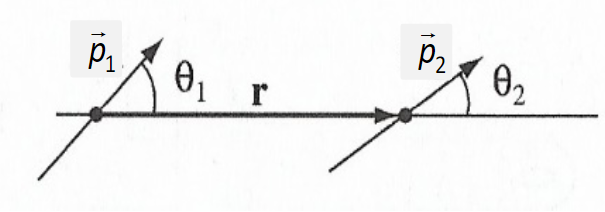
\includegraphics[scale=0.39]{DipoleInter.png}
\end{center}
\newpage

\section[Polarization]{\color{red}Polarization\color{black}}
When a piece of dielectric material is placed in an electric field, the field will induce a tiny dipole in nonpolar atoms, or molecules, and rotate the intrinsic dipole of polar molecules. The dipole moments tend to line them up along the field direction, leading to macroscopic dipole moment. The material is said to be polarized.\\

\begin{defn}
A measure of this polarization effect is called Polarization $\vec{P}$ as defined as the dipole moment per unit volume of the material.\\
\end{defn}

When the electric field, which the polarized material is placed in, is withdrawn, the polarization generally disappears. However, some materials may have memories to freeze in polarization.\\

\subsection*{Field Polarized Object}
Note that the potential at $\vec{r}$ produced by a dipole $\vec{p}$ at $\vec{r}'$ is given by the following:
\begin{align*}
V(\vec{r}) = \frac{1}{4\pi \epsilon_0}\vec{p}\cdot \left( \frac{\vec{r}-\vec{r}'}{|\vec{r}-\vec{r}'|^3}\right)
\end{align*}
Therefore the potential produced by a polarized object $V$ is given by:
\begin{align*}
V(\vec{r}) = \frac{1}{4\pi \epsilon_0}\int \frac{\vec{r}-\vec{r}'}{|\vec{r}-\vec{r}|^3}\cdot  d\vec{p} = \frac{1}{4\pi \epsilon_0}\int_V \frac{\vec{r}-\vec{r}'}{|\vec{r}-\vec{r}'|^3}\cdot \vec{P}(\vec{r}') \, d\tau' \tag{V}
\end{align*}
where the integration is over the volume of the object. 
\begin{center}
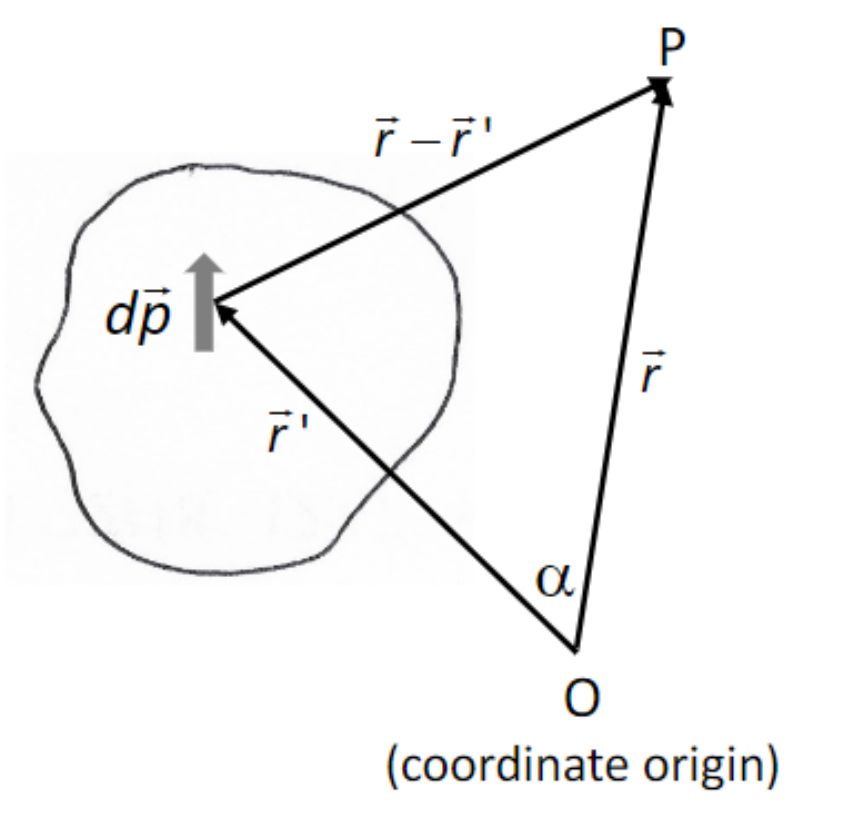
\includegraphics[scale=0.25]{IntegrateDipole.png}
\end{center}

\subsection*{Bound Charges}
Note that, in equation (V), we have:
\begin{align*}
\frac{\vec{r}-\vec{r}'}{|\vec{r}-\vec{r}'|^3} = \nabla' \left( \frac{1}{|\vec{r}-\vec{r}'|}\right)
\end{align*}
note that $\nabla'$ is operating on $\vec{r}'$, hence (V) can be written as:
\begin{align*}
V(\vec{r}) &= \frac{1}{4\pi \epsilon_0}\int_V \frac{\vec{r}-\vec{r}'}{|\vec{r}-\vec{r}'|^3}\cdot \vec{P}(\vec{r}') \, d\tau' \\
&= \frac{1}{4\pi \epsilon_0}\int_V \vec{P}(\vec{r}')\cdot \nabla'\left( \frac{1}{|\vec{r}-\vec{r}'|}\right) \, d\tau' \\
&= \frac{1}{4\pi \epsilon_0}\int_V \left(\nabla' \cdot \left(\frac{\vec{P}(\vec{r}')}{|\vec{r}-\vec{r}'|} \right) - \frac{\nabla' \cdot \vec{P}(\vec{r}')}{|\vec{r}-\vec{r}'|} \right) \, d\tau' \\
&= \frac{1}{4\pi \epsilon_0}\oint_S \frac{\vec{P}(\vec{r}')}{|\vec{r}-\vec{r}'|}\cdot d\vec{a}' + \frac{1}{4\pi \epsilon_0}\int_V \frac{-\nabla'\cdot \vec{P}(\vec{r}')}{|\vec{r}-\vec{r}'|}\, d\tau' \tag{VB}
\end{align*}
Now the first term in equation (VB) is a surface integral over the surface of the object, and the second term is a volume integral over the volume of the object. The first term is the potential of a surface charge and the second is the potential of a volume charge. Here we can define the bound surface density and the bound volume charge density.
\begin{defn}
The bound surface density is given by:
\begin{align*}
\sigma_b \coloneqq \vec{P}\cdot \vec{n}
\end{align*}
where $\vec{n}$ is the unit vector normal to the surface.\\
The bound volume density is given by the following:
\begin{align*}
\rho_b \coloneqq -\nabla \cdot \vec{p}
\end{align*}
\end{defn}
Then the potential of a polarized object is therefore given by:
\begin{align*}
V(\vec{r}) = \frac{1}{4\pi \epsilon_0}\oint_S \frac{\sigma_b(\vec{r}')}{|\vec{r}-\vec{r}'|}da' + \frac{1}{4\pi \epsilon_0}\int_V \frac{\rho_b(\vec{r'})}{|\vec{r}-\vec{r}'|}d\tau'
\end{align*}
The potential, and therefore the field, of a polarized object is the same as that produced by a volume of charge density $\rho_b = -\nabla \cdot \vec{P}$, plus that produced by a surface of charge density $\sigma_b = \vec{P}\cdot \vec{n}$. Note that the total bound charge, which is the sum of the volume and surface bound charges, vanishes:
\begin{align*}
\int_V \rho_b\,d\tau + \oint_S \sigma_b\,da = \int_V (-\nabla \cdot \vec{P})\, d\tau + \oint_S( \vec{P}\cdot \vec{n})\, da = -\oint_S \vec{P}\cdot d\vec{a} + \oint_S \vec{P}\cdot \vec{n}\, da = 0
\end{align*}

To get a better understanding of the bound surface charge, one can take a long string of physical dipoles that are aligned up head-to-tail. Along the line, the positive charge of one dipole cancels the negative charge of the dipole before it, leaving uncancelled charges at the two ends. These charges are bound to atoms or molecules. For a solid polarized object, the uncancelled charges are on the surface.

\begin{center}
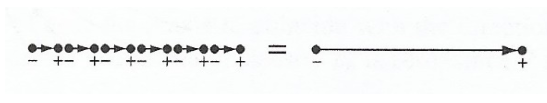
\includegraphics[scale=0.5]{SurfaceBound.png}
\end{center}

To get a better understanding of the bound volume charge, consider we were to produce polarizations with a non-zero divergence, the dipole moments
need to be spread out, which lead to concentration of negative or positive charges. This is the origin of the bound volume charge.
\begin{center}
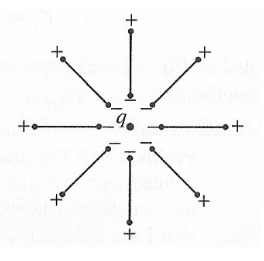
\includegraphics[scale=0.6]{volumeBound.png}
\end{center}

\subsection*{Fields of Uniformly Polarized Objects}
There are no volume bound charges inside uniformly polarized objects, but in general there will be bound surface charges. \\

For long cylinder, the bound surface charges are at the top and bottom of the cylinder with charges $q_b \approx \pm PA$. For a long cylinder, these bound charges are relatively small. Therefore, the field they produce are negligible. \\

For a thin wafer, the bound charges are on the surfaces of the thin wafer with uniform charge densities $\sigma_b = \vec{P}\cdot \vec{n} = \pm P$. Therefore, it is like a parallel-plate capacitor. The field it produces is given by:
\begin{align*}
\begin{cases}
E = \frac{P}{\epsilon_0} &\text{inside the wafer}\\
E = 0 & \text{outside the wafer}
\end{cases}
\end{align*}


\newpage
\section[Electric Displacement]{\color{red}Electric Displacement\color{black}}
The field due to polarization of the medium is the just the field of its bound charges. Hence in a space consisting of dielectric materials and other objects, the electric field is a combination of the field of the bound charges, and the field due to everything else, which we call the free charges. Consider the bound charges have charge density $\rho_b$, then the charge density in space can be written as the following:
$$\rho = \rho_b + \rho_f$$
here $\rho_f$ represents the charge density due to everything other than the bounded charges, that is, $\rho_f$ is the charge density due to free charges. \\

\note Dielectric materials, polarized or not, carry no free charges itself, it only carries bound charges, but there can be conductors or other materials embedded inside a dielectric material, which can carry free charges.\\

With Gauss's Law, we can write:
\begin{align*}
\epsilon_0 \nabla \cdot \vec{E} = \rho = \rho_b + \rho_f = -\nabla \cdot \vec{P}+\rho_f
\end{align*}
Here $\vec{E}$ is the total field due to both free and bound charges, rearranging we get:
\begin{align*}
\nabla \cdot (\epsilon_0 \vec{E}+\vec{P}) = \rho_f
\end{align*}

\begin{defn}
The electric displacement of a polarized object with dipole moment with unit are $\vec{P}$ is defined to be: 
$$\vec{D} = \epsilon_0  \vec{E} + \vec{P}$$
\end{defn}

Here we can write the following with Gauss's Law:
\begin{align*}
\nabla \cdot \vec{D} = \rho_f \qquad\qquad\qquad\qquad \oint_S \vec{D}\cdot d\vec{a} = Q_{\text{f,\ enc}}
\end{align*}
Here $Q_{\text{f, enc}}$ denotes the total free charges enclosed by the surface $S$.\\

Unlike the electric field, the electric displacement might have non-zero curl:
\begin{align*}
\nabla\times \vec{D} = \epsilon_0 \nabla \times \vec{E} + \nabla \times \vec{P} = \nabla \times \vec{P}
\end{align*}
The curl of polarization does not always vanish everywhere.\\

\note $\vec{D}$ vanishes inside a conductor.\\

\remark Since $\nabla \times \vec{D} $ is not always zero, the displacement cannot be expressed as a gradient of a scalar function, nor can it be derived in a way similar to the Columb's Law of $\vec{E}$. \\

\newpage
\section[Linear Dielectrics]{\color{red} Linear Dielectrics\color{black}}
For many dielectrics, the polarization is proportional to the field, provided that $\vec{E}$ is not too strong. That is, we can write:
\begin{align*}
\vec{P}\coloneqq \chi_e \epsilon_0 \vec{E}
\end{align*}
The proportional constant $\chi_e$ is called the electric susceptibility, a material property. Materials with this property are called linear dielectrics. \\

\note It should be noted that the field $\vec{E}$ here is the total field, including both the external field and the field resulting from the polarization.\\

For linear dielectrics with electric susceptibility $\chi_e$, we can write the following:
\begin{align*}
 \vec{D} = \epsilon_0 \vec{E} + \vec{P} = \epsilon_0 \vec{E} + \chi_e \epsilon_0 \vec{E} = \epsilon_0 (1+\chi_e) \vec{E}
\end{align*}
here we define: 
$$\epsilon \coloneqq  \epsilon_0 (1+\chi_e) $$
then we can write:
$$\vec{D} = \epsilon \vec{E}$$
$\epsilon$ is called the permittivity of the material. 
$$\epsilon_r \coloneqq 1+\chi_e$$ 
Here $\epsilon_r$ is called the dielectric constant, or the relative permittivity relative to free space.\\

In linear dielectrics, we can write Gauss's Law as the followings:
\begin{align*}
\nabla \cdot \vec{D} = \rho_f  \qquad\qquad\qquad \qquad \nabla \vec{E} = \frac{\rho_f}{\epsilon}
\end{align*}
\begin{align*}
\oint_S \vec{D}\cdot d\vec{a} = Q_{\text{f, enc}} \qquad\qquad\qquad\qquad \oint_S \vec{E} \cdot d\vec{a} = \frac{Q_{\text{f, enc}}}{\epsilon}
\end{align*}
Note that the electric displacement is determined by the free charges. \\

Since we have $\vec{D} = \epsilon\vec{E}$ in linear dielectrics, $\vec{D}$ appears to be curl-less in this case as we have:
$$\nabla \times \vec{D} = \epsilon\nabla \times \vec{E} = 0$$ 
This in fact is true if the space is entirely filled with one linear dielectric. However, it is not true if the space is only partially filled with dielectrics or filled with different dielectrics. \\

\begin{center}
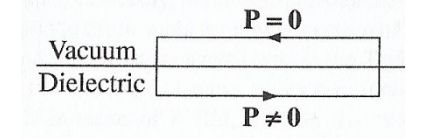
\includegraphics[scale=0.5]{curlD.png}
\end{center}

For instance, consider the loop $L$ straddling the boundary between a polarized linear dielectric and vacuum:
\begin{align*}
\oint_L \vec{D}\cdot d\vec{l} = \oint_L \vec{P}\cdot d\vec{l} \neq 0
\end{align*}
As the path integral doe not vanish, by Stoke's Theorem we know that the curl does not vanish.\\


If the space is entirely filled with one linear dielectric, then we can write:
\begin{align*}
\nabla \cdot \vec{E} = \frac{\rho_f}{\epsilon} \qquad\qquad\qquad\qquad\qquad \nabla \times \vec{E} = 0 
\end{align*}
and on the other hand, we have:
\begin{align*}
\nabla \cdot \vec{D} = \rho_f \qquad\qquad\qquad\qquad\qquad \nabla \times \vec{D} = 0
\end{align*}
In this case, $\vec{E}$ and $\vec{D}$ have identical properties other than a constant factor.\\

Now consider two cases, (1) the space is vacuum, and (2) the space is filled entirely by a linear dielectric. If the free charge distribution is the same, then $\vec{D}$ is the same for the two cases, and the electric field in the dielectric is reduced by a factor of the dielectric constant. That is, we have:
\begin{align*}
\vec{E}_{(2)} = \frac{\vec{E}_{(1)}\,\epsilon_0}{\epsilon}  = \frac{\vec{E}_{(1)}}{\epsilon_r}
\end{align*}
with $\vec{E}_{(1)}$ and $\vec{E}_{(2)}$ representing the fields in space (1) and space (2), respectively.\\

For a capacitor, the reduced field due to linear dielectric will reduce the voltage for the same charge, and therefore increase its capacitance $C = \epsilon_r C_0$, where $C_0$ is the capacitance without dielectric.\\
\newpage
\section[Boundary Conditions]{\color{red}Boundary Conditions\color{black}}
Let $E_{\perp}^{above}, E_{\perp}^{below}$ denote the normal component of the electric field, normal to the boundary of the martial, above and below the boundary of a material, respectively, with pointing from below to above as the positive direction. Let $E_{\parallel}^{above}, E_{\parallel}^{below}$ denote the parallel component of the electric field, parallel to the boundary of the material, above and below the boundary of a material, respectively. Let $D_{\perp}^{above}, D_{\perp}^{below}, E_{\parallel}^{above}, E_{\parallel}^{below}$ be defined similarly for electric displacement. Let $P_{\parallel}^{above}, P_{\parallel}^{below}$ denote parallel component of the polarization right above and below the boundary of the martial. Then in general, the electric displacement and electric field is subjected to the following conditions:
$$\oint_S \vec{D}\cdot d\vec{a} = Q_{\text{f, enc}} \qquad\qquad \Rightarrow \qquad \qquad D_{\perp}^{above} - D_{\perp}^{below} = \sigma_f$$
$$\oint_S \vec{E}\cdot d\vec{a} = \frac{Q_{\text{enc}}}{\epsilon_0} \qquad\qquad\ \ \Rightarrow  \qquad \qquad E_{\perp}^{above} - E_{\perp}^{below} = \frac{\sigma}{\epsilon_0}$$
where $\sigma_f$ is the free surface charge on the material, and $\sigma$ include both free and bound charges on the surface of the martial. \\

On the other hand, we can write:
$$\oint_L \vec{D}\cdot d\vec{l} = \oint_L \vec{P}\cdot d\vec{l} \qquad\qquad\Rightarrow\qquad\qquad D_{\parallel}^{above} - D_{\parallel}^{below} = P_{\parallel}^{above} - P_{\parallel}^{below}$$
$$\oint_L \vec{E}\cdot d\vec{l} = 0 \qquad\qquad\qquad \ \ \ \Rightarrow\qquad\qquad E_{\parallel}^{above} - E_{\parallel}^{below} = 0 \qquad\qquad\qquad$$
Here we get a boundary condition, with $\vec{n}$ being a vector normal to the surface:
\begin{align*}
D_{\perp}^{above} - D_{\perp}^{below} = \sigma_f
\end{align*}


In linear dielectrics, we can write the following:
\begin{align*}
\epsilon_{above}\, E_{\perp}^{above} - \epsilon_{below}\, E_{\perp}^{below} = \sigma_f
\end{align*}
where $\epsilon_{above}, \epsilon_{below}$ are the permittivity of the materials above and below the surface, respectively.\\

Particularly at a conductor-dielectric boundary, the electric field right inside the dielectric material is found to be the following, with $\epsilon$ being the permittivity of the dielectric material:
\begin{align*}
\vec{E}_{\text{dielectric}} = \frac{\sigma_f}{\epsilon} \, \vec{n} \qquad\qquad\qquad \qquad \sigma_f = \epsilon\vec{E}\cdot \vec{n} = -\epsilon\,  \frac{\partial V}{\partial n}
\end{align*}
where $\vec{n}$ point in the direction from the conductor to the dielectric, normal to the boundary surface. \\


\newpage
\section[Properties of Linear Dielectrics]{\color{red}Properties of Linear Dielectrics \color{black}}
In linear dielectrics, the bound volume charge can be written as the following:
\begin{align*}
\rho_b = -\nabla \cdot \vec{P} = -\nabla \cdot (\chi_e \epsilon_0 \vec{E}) = -\nabla \cdot \left(\frac{\chi_e \, \epsilon_0}{\epsilon}\vec{D}\right) = - \frac{\chi_e}{1+\chi_e} (\nabla \cdot \vec{D}) = -\frac{\chi_e}{1+\chi_e}\rho_f
\end{align*}
Hence we see that, in linear dielectrics, the bound volume charge density is proportional to the free volume charge density. Consequently, the charge density in linear dielectric material is effectively reduced by a factor of the dielectric constant. Here we can write:
\begin{align*}
\rho = \rho_b + \rho_f = \frac{\rho_f}{1+\chi_e} = \frac{\rho_f}{\epsilon_r}
\end{align*}
\note Unless free charge is embedded in the linear dielectric material, we have $\rho = 0$, and any net charge must reside at the surface of the material.\\

For bound surface charge density, we can write the following:
\begin{align*}
\sigma_b = \vec{P}\cdot \vec{n} = (\chi_e \epsilon_0 \vec{E}) \cdot \vec{n} = \left( \frac{\chi_e \epsilon_0}{\epsilon} \vec{D}\right) \cdot \vec{n} = \frac{\chi_e}{1+\chi_e} D_{\perp}
\end{align*} 
where $\vec{n}$ is the unit vector point normal to the surface of the dielectric material, and pointing outwards. $D_\perp$ is the normal component of the electric displacement at the surface of the dielectric material.\\



At a conductor-dielectric boundary, we can write the following:
\begin{align*}
D_{\perp}^{above} - D_{\perp}^{below} = \sigma_f \qquad  D_{\perp}^{above} = 0 \qquad D_{\perp}^{below} = D_{\perp} \qquad \Rightarrow \qquad D_{\perp} = -\sigma_f
\end{align*}
Thus we see that:
\begin{align*}
\sigma_b = -\frac{\chi_e}{1+\chi_e}\,D_{\perp} =-\frac{\chi_e}{1+\chi_e}\,\sigma_f \qquad \Rightarrow \qquad \sigma = \sigma = \sigma_b + \sigma_f = \frac{\sigma_f}{1+\chi_e} = \frac{\sigma_f}{\epsilon_r}
\end{align*}
At a conductor-dielectric boundary, we see that the bound surface charge density on the dielectric material is proportional to the free charge density on the conducting material. However, we note that at a dielectric-dielectric boundary, there may be bound surface charge without free surface charges.

\begin{center}
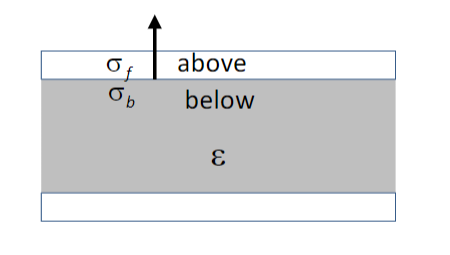
\includegraphics[scale=0.5]{CDboundary.png}
\end{center}


\note Dielectric effectively reduces the free charge density by a factor of the dielectric constant.\\

\subsection*{Boundary Value Problems with Linear Dielectrics}

Since the potential is defined from electric field, Poisson's Equation is still valid in dielectrics:
\begin{align*}
\nabla^2 V = -\frac{\rho}{\epsilon_0}
\end{align*}
where $\rho$ is the total charge density. In linear dielectric, we can write the following:
\begin{align*}
\rho = \frac{\rho_f}{\epsilon_r} = \frac{\epsilon_0\, \rho_f}{\epsilon} \qquad \qquad \Rightarrow \qquad \qquad \nabla^2 V = -\frac{\rho_f}{\epsilon} \tag{PD}
\end{align*}
Since there is no free charges inside the dielectrics, equation (PD) reduces to the Laplace's Equation:
\begin{align*}
 \nabla^2 V = 0
\end{align*}

In linear dielectrics, the boundary conditions can be written as the following:
\begin{align*}
\epsilon_{above}\, E_{\perp}^{above} - \epsilon_{below}\, E_{\perp}^{below} = \sigma_f \qquad \Rightarrow \qquad \epsilon_{above}\, \left(\frac{\partial V}{\partial n} \right)^{above} - \epsilon_{below}\, \left(\frac{\partial V}{\partial n} \right)^{below} = -\sigma_f
\end{align*}



\note The potential $V$ is still continuous at the boundary.\\

In particular, at a conductor-dielectric surface, we have:
\begin{align*}
 \epsilon\, \frac{\partial V}{\partial n} = -\sigma_f
\end{align*}
where $\vec{n}$ is the unit vector normal to the surface of the conductor, pointing into the dielectric, and $\epsilon$ is the permittivity of the dielectric.\\

At a dielectric-dielectric surface, we have the following instead:
\begin{align*}
\epsilon_{above}\, \left(\frac{\partial V}{\partial n} \right)^{above} = \epsilon_{below}\, \left(\frac{\partial V}{\partial n} \right)^{below}
\end{align*}
\newpage

\section[Energy in Dielectric Systems]{\color{red}Energy in Dielectric Systems\color{black}}
Without dielectrics, the energy stored in the charge distribution, or the field $F$, is given by the following:
\begin{align*}
W = \frac{1}{2}\int_F \rho V\, d\tau = \frac{\epsilon_0}{2} \int_F ||\vec{E}||^2 \, d\tau
\end{align*}
In the presence of dielectrics, energy is, in addition, stored in the polarization. Again starting with the assembly of a free charge distribution $\rho_f$, the work needs to be done is still given by:
\begin{align*}
W = \frac{1}{2}\int \rho_f V\, d\tau = \frac{1}{2} (\nabla \cdot \vec{D}) \, V \, d\tau = \frac{1}{2}\int (\nabla \cdot (\vec{D}V) - \vec{D}\cdot (\nabla V)) \, d\tau \tag{UD}
\end{align*}
with the integral over the charge distribution. Noe that it can be extended to the whole space by letting $\rho_f$ being zero outside the charge distribution. Note that we have $\vec{E}= -\nabla{V}$, then equation (UD) becomes the following:
\begin{align*}
W = \frac{1}{2}\oint_S V \vec{D}\cdot d\vec{a}+ \frac{1}{2}\int_A \vec{D}\cdot \vec{E}\,d\tau
\end{align*}
where $A$ is the whole space, and $S$ is the "surface" of the whole space. As seen before, we know that $D \propto \frac{1}{r^2}$ and $V \propto \frac{1}{r}$, hence $\int_S V\vec{D}\cdot d\vec{a}$ vanishes. Thus with dielectrics, the energy stored in the configuration is given by:
\begin{align*}
W = \frac{1}{2}\int_A \vec{D} \cdot \vec{D}\, d\tau
\end{align*}
where $A$ is the whole space, and here for linear dielectrics, we have:
\begin{align*}
W = \frac{\epsilon}{2} \int_V E^2\, d\tau\qquad\qquad\qquad\qquad\qquad u_E = \frac{1}{2}\epsilon E^2
\end{align*}
Note that this is the energy stored in a dielectric polarized by an external field, not the energy of an object with frozen-in polarization without an external field.\\

\subsection*{Forces on Dielectrics}
The electrostatic pressure on a conducting surface $P = \frac{\epsilon_0 \sigma^2}{2}$ is an outward force that tends to draw the conductor into the field. Similarly, the electric field tends to draw dielectrics into the field.\\

For a parallel-plate capacitor, the field is uniform in the region between the two plates and zero outside in the idealized case. If this is true, the line integral given by:
\begin{align*}
\oint_L \vec{E} \cdot d\vec{l}
\end{align*}
will not vanish if the loop $L$ straddles the capacitor boundary. As a result, the curl-less nature of the electrostatic field guarantees non-zero fringing field outside the parallel-plate capacitor. The field cannot vanish abruptly at the edge. This non-uniform fringing field will exert a force on dielectrics if it were inserted from the edge of the parallel-plate capacitor, pulling it into the capacitor.\\

\begin{center}
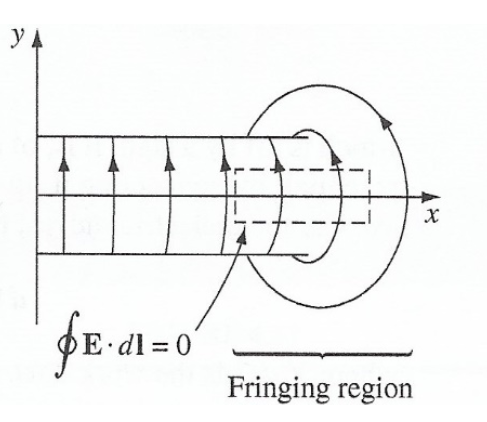
\includegraphics[scale=0.5]{Fringing.png}
\end{center}

The fringing field is difficult to calculate. However, we can bypass it by deriving the force from the energy taking advantage of the conservative nature of the electrostatic force:
$$\vec{F} = -\nabla U$$
where $U$ is the potential energy. In previous discussion, we have used $W$ for the work done to the system which turns into the electrostatic energy. Here $U$ also denote the electrostatic energy, which is the energy stored in the field.\\


\newpage
\chapter{Magnetostatics}

A stationary charge produces only an electric field. A moving charge will generate 
electric current which in turn produces, in addition, a magnetic field.  

\begin{defn}
Steady charge motion, steady currents, which produce magnetic fields that are constant in time is the study of Magnetostatics.
\end{defn}


\section[Magnetic Force]{\color{red}Magnetic Force\color{black}}

\begin{thm}
A particle with charge $Q$ moving with a velocity $\vec{v}$ inside a magnetic field $\vec{B}$ will experience a magnetic force given by the following:
\begin{align*}
\vec{F}_{mag} = Q \vec{v}\times \vec{B} \tag{M}
\end{align*}
\end{thm}
The unit for measuring the strength of a magnetic field is Tesla, denoted as $[T]$. 

The magnetic force, as given in equation (M), is perpendicular to both the velocity and the magnetic field, and because of this, the magnetic force does no work to the charge. That is, the magnetic force cannot change the speed of the particle, but it can change the direction of the velocity of the particle. 
\begin{align*}
dW = \vec{F}_{mag} \cdot d\vec{l} = \vec{F}_{mag} \cdot \frac{d\vec{l}}{dt}\, dt = Q(\vec{v}\times \vec{B}) \cdot \vec{v}\, dt = 0
\end{align*}
In the presence of both electric and magnetic fields, the net force on a charge $Q$ with velocity $\vec{v}$ is then given by:
\begin{align*}
\vec{F} = Q (\vec{E} + \vec{v}\times \vec{B} \tag{MB}
\end{align*}
Equation (MB) is known as the Lorentz Force Law.\\

\newpage
\section[Electric Currents]{\color{red}Electric Currents\color{black}}

\begin{defn}
Current, denoted as $I$, is the charge passing through per unit time.
\end{defn}

In the SI unit system, current is measured in $C/s$, or Amperes, denoted as $A$, with $1\, A = 1\, C/s$. Current is a vector, which direction is determined by the direction of the charge motion.\\

Line current $\vec{I}$ is the charge passing a given point on a wire per unit time. A line charge of density $\lambda$ traveling at a velocity $\vec{v}$ constitutes a line current $\vec{I} = \lambda \vec{v}$. \\



For currents flowing over a surface, surface current density, denoted as $\vec{K}$ is defined as the current per unit length perpendicular to the current flow:
\begin{align*}
 \vec{K}\coloneqq \frac{d\vec{I}}{dl_{\perp}}
\end{align*}
for surface charges with density $\sigma$ moving wit a velocity $\vec{v}$, we have $\vec{K} = \sigma \vec{v}$. 


\begin{center}
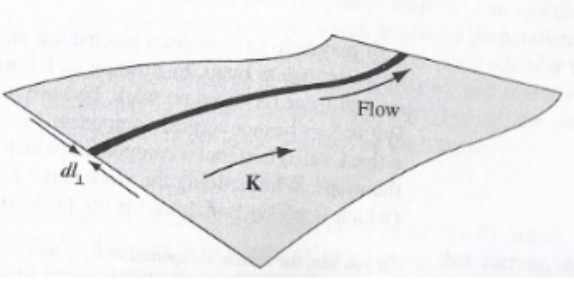
\includegraphics[scale=0.39]{surfaceCurrent.png}
\end{center}

For currents flowing over a volume, the volume current density is defined as the current per unit area perpendicular to the current flow:
\begin{align*}
 \vec{J} = \frac{d\vec{I}}{da_{\perp}}
\end{align*}
Hence the current flowing across a surface area $S$ is given by:
\begin{align*}
 I = \int_S \vec{J} \cdot d\vec{a}
\end{align*}
For volume charges with density $\rho$ moving at a velocity $\vec{v}$, we have $\vec{J} = \rho \vec{v}$.

\begin{center}
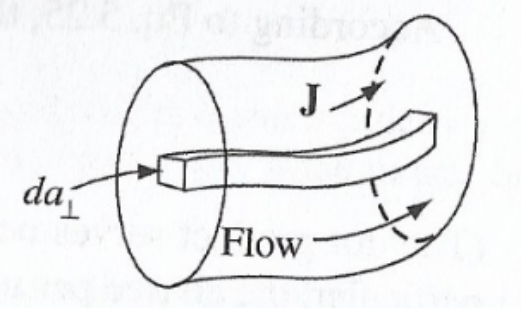
\includegraphics[scale=0.39]{volumeCurrent.png}
\end{center}


In a conductor, the charges in motion are actually the  negatively  charged electrons. In this case, the current direction is opposite to that of the electron motion.\\

A small segment of a wire $dl$ with charge $dq$ moving at $\vec{v}$ in magnetic field $\vec{B}$ will experience a magnetic force $d\vec{F}_{mag} = dq(\vec{v}\times \vec{B})$. Thus the force on a current-carrying wire in a magnetic field $\vec{B}$ is given by:
\begin{align*}
 \vec{F}_{mag} = \int(\vec{v}\times \vec{B}) \, dq = \int(\vec{v}\times \vec{B}) \lambda \, dl = \int(\vec{I}\times \vec{B})\, dl = I \int d\vec{l}\times \vec{B}
\end{align*}
Note that for a wire, the directions of $d\vec{l}$ and $\vec{I}$ are interchangeable assuming the line integral follows the current direction. \\

The force on a surface current is given by the following:
\begin{align*}
 \vec{F}_{mag} = \int(\vec{v}\times \vec{B}) \, dq = \int(\vec{v}\times \vec{B}) \, \sigma \, da = \int(\vec{K}\times \vec{B}) \, da
\end{align*}

The force on a volume current is given by the following:
\begin{align*}
\vec{F}_{mag} = \int(\vec{v}\times \vec{B}) \, dq = \int (\vec{v}\times \vec{B}) \, \rho \, d\tau = \int(\vec{J}\times \vec{B}) \, d\tau
\end{align*}

\subsection*{Continuity Equation}
Charge conservation requires that the charge flowing out a volume should be at the expenses of the charge inside the volume, that is, we can write:
\begin{align*}
\oint_S \vec{J}\cdot d\vec{a} = -\frac{dQ}{dt} \qquad \qquad \qquad \Rightarrow\qquad\qquad\qquad \int_V \nabla\cdot \vec{J}\, d\tau = -\frac{d}{dt} \int_V \rho \, d\tau = -\int \left( \frac{\pd \rho}{\pd t}\right)\, d\tau
\end{align*}
Here $S$ is a surface and $V$ is the volume enclosed by $S$. Since this equality applies to any volume $V$, we conclude the following:
\begin{align*}
\nabla \cdot \vec{J} + \frac{\pd \rho}{\pd t} = 0 \tag{CE}
\end{align*}
Equation (CE) is called the continuity equation, a statement of the charge conservation.\\

\subsection*{Steady Currents}
Stationary charges produce electric fields that are constant in time; hence the term electrostatics. Steady currents produce magnetic fields that are constant in time; the theory of steady currents is called magnetostatics.\\

A steady current is a continuous flow that has been going on forever,  without change and without charge piling up anywhere. Formally, electrostatics and magnetostatics both satisfy the equations:
\begin{align*}
\frac{\pd \rho}{\pd t} = 0 \qquad\qquad\qquad \frac{\pd \vec{J}}{\pd t} = 0 \qquad\qquad\qquad \nabla \cdot \vec{J} = 0
\end{align*}
at all places and all times. In reality, no current is truly steady. But as long as the change is gradual, the steady current is a good approximation for many systems. Here gradual means that time of change is must longer than the time of a measurement.\\

\newpage
\section[Hall Effect]{\color{red}Hall Effect \color{black}}
Hall effect refers to the phenomena of a voltage difference, called the Hall voltage, developed across a conducting slab when an electric current flows perpendicular to an external magnetic field. \\

\begin{center}
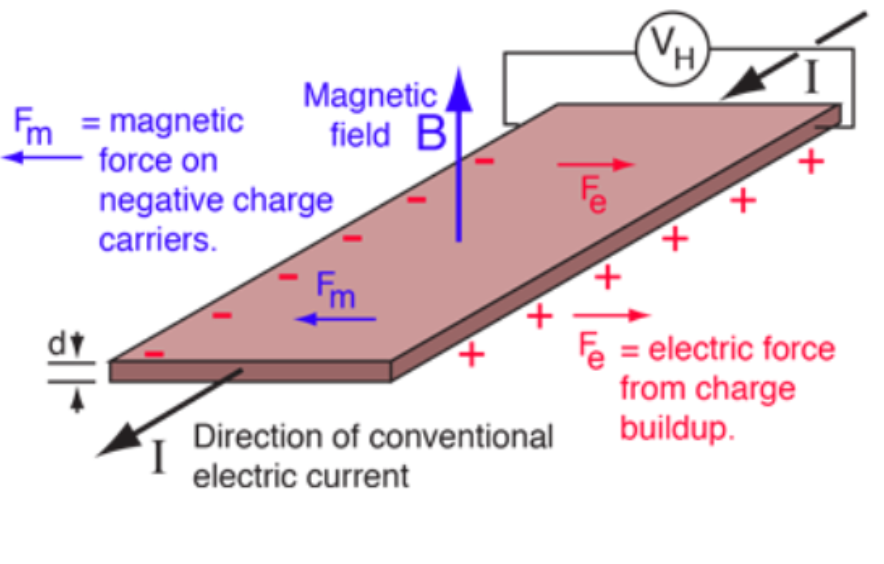
\includegraphics[scale=0.5]{hall.png}
\end{center}

Let $e$ denote the magnitude of the charge of an electron. When a current is turned on, the electrons will experience a magnetic force given by:
\begin{align*}
\vec{F}_m = -e \vec{v}\times \vec{B}
\end{align*}
where $\vec{v}$ is the velocity of the electron and $\vec{B}$ is the magnetic field. Here $\vec{F}_m$ is perpendicular to both the current and $\vec{B}$, leading to the accumulation of charges at the edges of the slab. The charges will in turn establish an electric field that exerts an electric force on the electrons, opposite to the magnetic force,, given by:
\begin{align*}
\vec{F} = -e(\vec{E}+\vec{v}\times \vec{B})
\end{align*}

Here an equilibrium is reached when the two forces balanced out:
\begin{align*}
\vec{E} = -\vec{v}\times \vec{B}
\end{align*}
The voltage developed between the edges of the slab is then given by:
\begin{align*}
V_H = Ew = vwB
\end{align*}
where $w$ is the width of the slab, measuring the length in the direction parallel to the electric field. Note that we can write the following:
\begin{align*}
I = JA = (\rho v)(wd) = n_e evwd  \qquad \qquad \Rightarrow \qquad vw = \frac{I}{n_e ed}
\end{align*}
where $n_e$ is the density of the mobile electrons, $A$ is the cross-sectional area of the slab, and $d$ is the thickness of the slab. Thus the Hall voltage is given by the following:
\begin{align*}
V_H = \frac{1}{n_e e} \frac{IB}{d} = R_H\, \frac{IB}{d}\qquad\qquad\qquad \qquad \qquad R_H \coloneqq \frac{1}{n_e e}
\end{align*}
here $R_H$ is called the Hall coefficient. 

\newpage
\section[Biot-Savart Law]{\color{red}Biot-Savart Law \color{black}}
\begin{thm}[Biot-Savart Law]
Biot-Savart Law is named after French Mathematicians and Physicists Jean-Baptiste Biot (1774-1862) and Felix Savart (1791-1841). The law states that currents produce magnetic field. The field produced by a steady line current at $\vec{r}$ is given by the Biot-Savart Law:
\begin{align*}
B(\vec{r}) = \frac{\mu_0 I}{4\pi} \left(\int_L d\vec{l}' \times \frac{(\vec{r}-\vec{r}')}{|\vec{r} - \vec{r}'|^3}\right) = \frac{\mu_0}{4\pi} \int_L \vec{I}(\vec{r}') \times \frac{(\vec{r}-\vec{r}')}{|\vec{r}-\vec{r}'|^3}\, dl'
\end{align*}
where $L$ is along the path of the current, note here we have $I d\vec{l}= \vec{I}\,dl$, and in differential form:
\begin{align*}
dB(\vec{r}) = \frac{\mu_0 I}{4\pi}\, d\vec{l}' \times \left(\frac{\vec{r}-\vec{r}'}{|\vec{r}-\vec{r}'|^3} \right)
\end{align*}
Here $\mu_0 = 4\pi \cdot 10^{-7}\, N/A^2$ is a constant of the space called the permeability. 
\end{thm}

\begin{center}
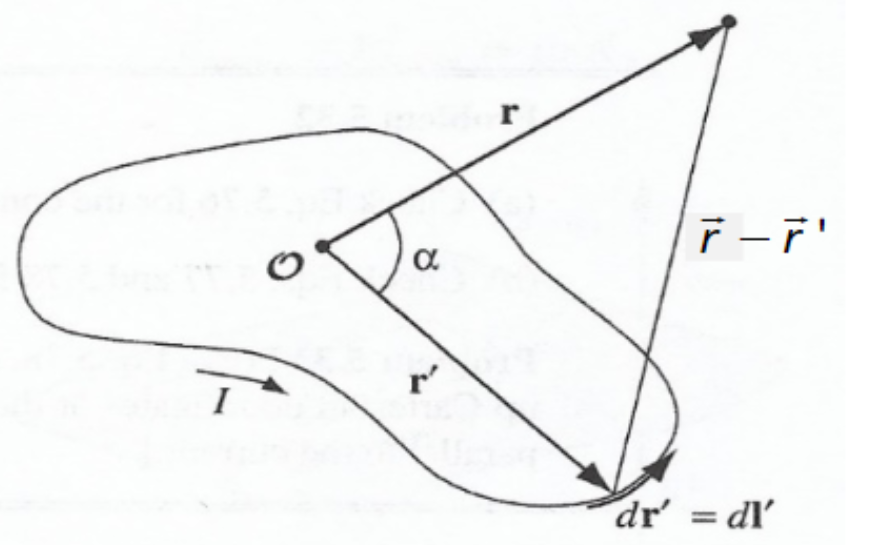
\includegraphics[scale=0.3]{BSlaw.png}
\end{center}

In the SI unit, the magnetic field is measured in $N/(A\cdot m)$, and is defined as Tesla, denoted as $T$, with $1\, T = 1\, N/(A\cdot m)$. Another unit for magnetic field is Gauss, denoted as $G$, with $1\, G = 10^{-4}\, T$.\\

For currents in surface $S$ and volume $V$, the Biot-Savart Law becomes the following:
\begin{align*}
B(\vec{r}) = \frac{\mu_0}{4\pi}\int_S \vec{K}(\vec{r}') \times \frac{(\vec{r}-\vec{r}')}{|\vec{r} - \vec{r}'|^3}\, da'\qquad\qquad\qquad B(\vec{r}) = \frac{\mu_0}{4\pi}\int_V \vec{J}(\vec{r}') \times \frac{(\vec{r}-\vec{r}')}{|\vec{r} - \vec{r}'|^3}\, d\tau'
\end{align*}
Here we notice that the cross product in the Biot-Savart Law makes the field direction perpendicular to both the current and the position vector, and is determined by the right-hand rule.\\

\note Like Coulomb's law, Biot-Savart law is a fundamental law of physics and cannot be derived from any other law. It is validity can only be confirmed through experiments.\\

\example\\
One can derive from the Biot-Savart Law that the parallel currents attract and anti-parallel currents repel with the force per unit length given by the following:
\begin{align*}
F = \frac{\mu_0}{2\pi}\frac{I_1 I_2}{d}
\end{align*}
where $d$ is the separation of the two currents and $I_1$, $I_2$ represents the magnitude of the two currents, respectively.\\

\begin{center}
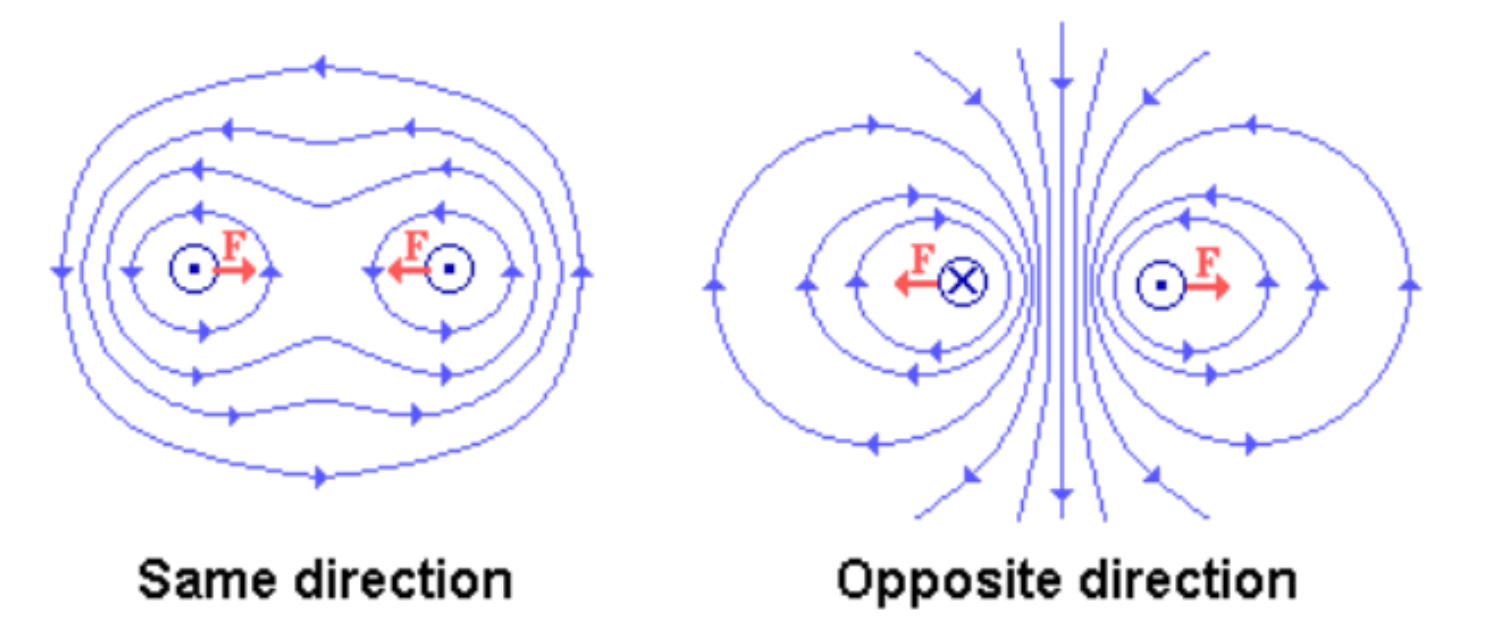
\includegraphics[scale=0.25]{twoCurrents.png}
\end{center}
\newpage

\subsection*{Curl and Divergence of the Magnetic Field}
Here we can derive the divergence of a magnetic field from the Biot-Savart Law. First we note that we can write the following:
\begin{align*}
\nabla \times \frac{(\vec{r}-\vec{r}')}{|\vec{r}-\vec{r}'|^3} = 0 \qquad\qquad\qquad \nabla \cdot   \frac{(\vec{r}-\vec{r}')}{|\vec{r}-\vec{r}'|^3} = 4\pi \delta^3 (\vec{r} - \vec{r}')
\end{align*}
the operator $\nabla$ acts on $\vec{r}$ here, and the delta function $\delta^3$ is defined by:
\begin{align*}
\delta^3 : \R^3 \to 0  \ \ \ \vec{r} \mapsto \begin{cases} 
0 & \vec{r}\neq \vec{r}'\\
\infty & \vec{r} = \vec{r}'
\end{cases}
\end{align*}
Now the divergence of the magnetic field is given by the following, with $\nabla$ acting on $\vec{r}$:
\begin{align*}
\nabla \cdot \vec{B}(\vec{r}) =\nabla \cdot \left( \frac{\mu_0}{4\pi}\int \vec{J}(\vec{r}')\times \frac{( \vec{r}- \vec{r}')}{|\vec{r}-\vec{r}'|^3} \, d\tau'\right)=\frac{\mu_0}{4\pi}\int \nabla \cdot \left(\vec{J}(\vec{r}')\times \frac{( \vec{r}- \vec{r}')}{|\vec{r}-\vec{r}'|^3}\right) \, d\tau'
\end{align*}
while we have:
\begin{align*}
 \nabla \cdot \left(\vec{J}(\vec{r}')\times \frac{( \vec{r}- \vec{r}')}{|\vec{r}-\vec{r}'|^3}\right) = \left(\nabla \times \vec{J}(\vec{r}')\right) \cdot \left( \frac{\vec{r}-\vec{r}'}{|\vec{r}-\vec{r}'|^3}\right) - \vec{J}(\vec{r}') \cdot \left(\nabla \times  \frac{(\vec{r}-\vec{r}')}{|\vec{r}-\vec{r}'|^3}\right) = 0 
\end{align*}
It follows that we have:
\begin{align*}
\nabla \cdot \vec{B} = 0
\end{align*}

On the other hand, we can compute the curl of the magnetic field:
\begin{align*}
\nabla \times \vec{B}(\vec{r}) =\nabla \times \left( \frac{\mu_0}{4\pi}\int \vec{J}(\vec{r}')\times \frac{( \vec{r}- \vec{r}')}{|\vec{r}-\vec{r}'|^3} \, d\tau'\right)=\frac{\mu_0}{4\pi}\int \nabla \times \left(\vec{J}(\vec{r}')\times \frac{( \vec{r}- \vec{r}')}{|\vec{r}-\vec{r}'|^3}\right) \, d\tau'
\end{align*}
where we have:
\begin{align*}
 \nabla \times \left(\vec{J}(\vec{r}')\times \frac{( \vec{r}- \vec{r}')}{|\vec{r}-\vec{r}'|^3}\right) = \vec{J}(\vec{r}')\left( \nabla \cdot \frac{(\vec{r}-\vec{r}')}{|\vec{r}-\vec{r}'|^3}\right) - \left(\vec{J}(\vec{r}')\cdot \nabla\right)\left( \frac{\vec{r}-\vec{r}'}{|\vec{r}-\vec{r}'|^3}\right)
\end{align*}
Here we can write:
\begin{align*}
\nabla \times \vec{B}(\vec{r}) &=\int \left(\vec{J}(\vec{r}')\left( \nabla \cdot \frac{(\vec{r}-\vec{r}')}{|\vec{r}-\vec{r}'|^3}\right)-\left(\vec{J}(\vec{r}')\cdot \nabla\right)\left( \frac{\vec{r}-\vec{r}'}{|\vec{r}-\vec{r}'|^3}\right)\right) \, d\tau \\&= \int \left(\vec{J}(\vec{r}')\left( \nabla \cdot \frac{(\vec{r}-\vec{r}')}{|\vec{r}-\vec{r}'|^3}\right) \right) \, d\tau -\int \left( \left(\vec{J}(\vec{r}')\cdot \nabla\right)\left( \frac{\vec{r}-\vec{r}'}{|\vec{r}-\vec{r}'|^3}\right)\right) \, d\tau\\
&=\mu_0 \vec{J}(\vec{r}) + 0 \\
&=  \mu_0 \vec{J}(\vec{r}) 
\end{align*}
It follows that we have:
\begin{align*}
\nabla \times \vec{B} = \mu_0 \vec{J}
\end{align*}


\newpage
\section[Ampere's Law]{\color{red}Ampere's Law\color{black}}
\begin{thm}
Ampere's Law is named after French mathematician and physicist Andre-Marie Ampere (1775-1836), while we note that Ampere's Law is derived from Biot-Savart Law. Ampere's Law is stated as the following:
\begin{align*}
\nabla \times \vec{B}(\vec{r}) = \mu_0 \vec{J}(\vec{r})
\end{align*}
\end{thm}

Taking the surface integral, we get the following:
\begin{align*}
\int_S (\nabla \times \vec{B}) \cdot d\vec{a} = \mu_0 \int_S \vec{J}\cdot d\vec{a}
\end{align*}
Note that we can write:
\begin{align*}
\int_S \vec{J}\cdot d\vec{a} = I_{\text{enc}}\qquad\qquad\qquad\int_S (\nabla \times \vec{B}) \cdot d\vec{a}  = \oint_L \vec{B}\cdot d\vec{l} = \mu_0 I_{\text{enc}}
\end{align*}
The line integral loop $L$, which is the boundary of $S$, is called  Amperian loop and $I_{\text{enc}}$ is the total current enclosed by the loop which is the total current passing through any surface bounded by the loop with the direction determined by the right-hand rule.\\

\begin{center}
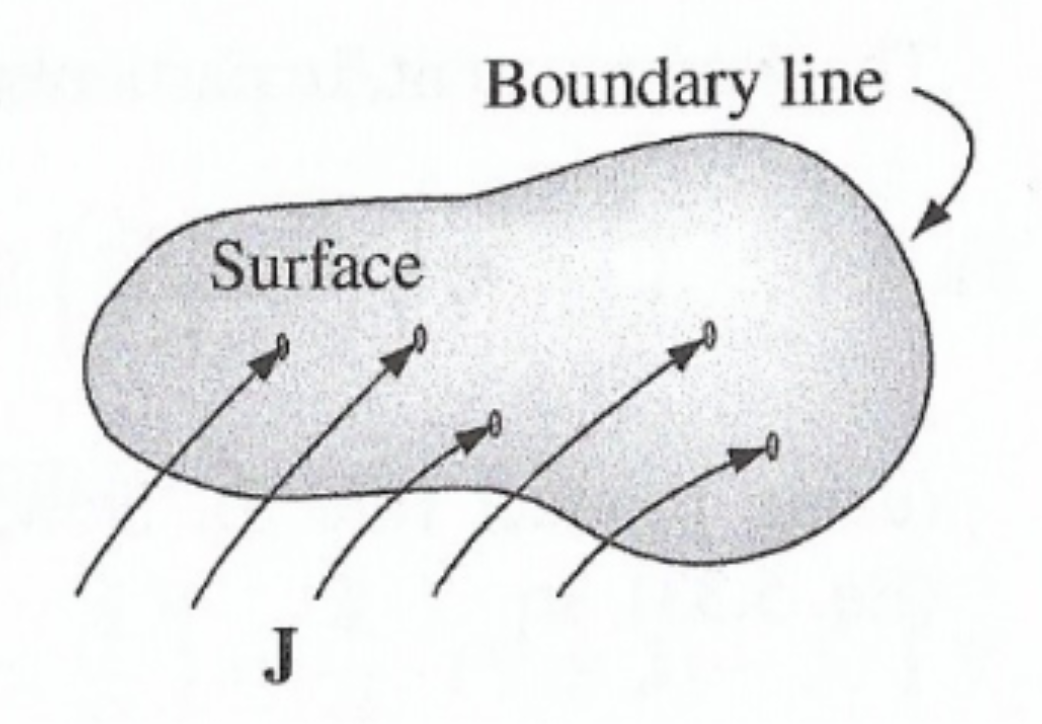
\includegraphics[scale=0.19]{AmpereLaw.png}
\end{center}

\note Ampere’s law plays the same role in magnetostatics as Gauss’s law plays in electrostatics. It can be used to compute magnetic field in certain geometries with symmetry.\\

\example\\
The electric field of a line charge of density $\lambda$ is given by the following:
\begin{align*}
\vec{E}(s) = \frac{1}{2\pi \epsilon_0}\frac{\lambda}{s}\, \hat{s}
\end{align*}
where $\vec{s}$ is the distance from the line charge. \\
While for a line current $I$, the magnetic field created by the line current is given by:
\begin{align*}
\vec{B}(s) = \frac{\mu_0}{2\pi}\frac{I}{s}\,\hat{\phi}
\end{align*}
where $\vec{s}$ is the distance from the line current. \\

\newpage
\section[Magnetic Vector Potential]{\color{red}Magnetic Vector Potential\color{black}}
Since we have $\nabla \cdot \vec{B} = 0$, the magnetic field can be expressed as a curl of a vector potential $\vec{A}(\vec{r})$, which is called the magnetic vector potential. We can write:
\begin{align*}
\vec{B}(\vec{r}) = \nabla \times \vec{A}(\vec{r})
\end{align*}
note that $\nabla \cdot (\nabla \times \vec{A}) = 0$. Now we can write the following through Amperes's Law:
\begin{align*}
\nabla \times \vec{B} = \nabla \times (\nabla \times \vec{A}) = \nabla(\nabla \cdot \vec{A}) - \nabla^2 \vec{A} = \mu_0 \vec{J}
\end{align*}
The vector potential $\vec{A}$ is not uniquely determined, adding a gradient $\nabla \Psi$ does not affect the magnetic field:
\begin{align*}
\vec{B} = \nabla \times (\vec{A} + \nabla \Psi) = \nabla \times \vec{A}
\end{align*}
This freedom of adding a gradient is often exploited to require $\nabla \cdot \vec{A} = 0$, which is known as the Coulomb gauge, which this choice, Ampere's Law becomes the following form:
\begin{align*}
\nabla^2 \vec{A} = -\mu_0 \vec{J} \tag{PA}
\end{align*}
Note that here we can write the magnetic flux through a surface $S$ in terms of $\vec{A}$:
\begin{align*}
\Phi = \int_S \vec{B}\cdot d \vec{a} = \int_S \nabla \times \vec{A}\cdot d\vec{a} = \oint_L \vec{A}\cdot d\vec{l}
\end{align*}
where $L$ is the boundary of $S$.\\

Note that equation (PA) gives a Poisson's Equation for the vector potential. Its solution can be obtained by comparing with the scalar potential for the electric field. For a localized current distribution $\vec{J}(\vec{r})$, the solution for $\vec{A}(\vec{r})$ is given by the following:
\begin{align*}
\vec{A}(\vec{r}) = \frac{\mu_0}{4\pi}\int_V \frac{\vec{J}(\vec{r}')}{|\vec{r}-\vec{r}'|}\, d\tau'
\end{align*}
where $V$ is a localized space. Extended to localized surface currents $S$ and line currents $L$, we have:
\begin{align*}
\vec{A}(\vec{r}) = \frac{\mu_0}{4\pi}\int_S \frac{\vec{K}(\vec{r}')}{|\vec{r}-\vec{r}'|}\, da' \qquad\qquad\qquad\qquad \vec{A}(\vec{r}) = \frac{\mu_0}{4\pi}\int_L \frac{\vec{I}(\vec{r}')}{|\vec{r}-\vec{r}'|}\, dl' = \frac{\mu_0 I}{4\pi}\int_L \frac{d\vec{l}'}{|\vec{r}-\vec{r}'|}
\end{align*}
The vector potential is generally in the current direction and contains everything to know about the magnetic field, but it is not as useful as the scalar potential in the electric case as the trade off is between the two vectors.\\

\begin{center}
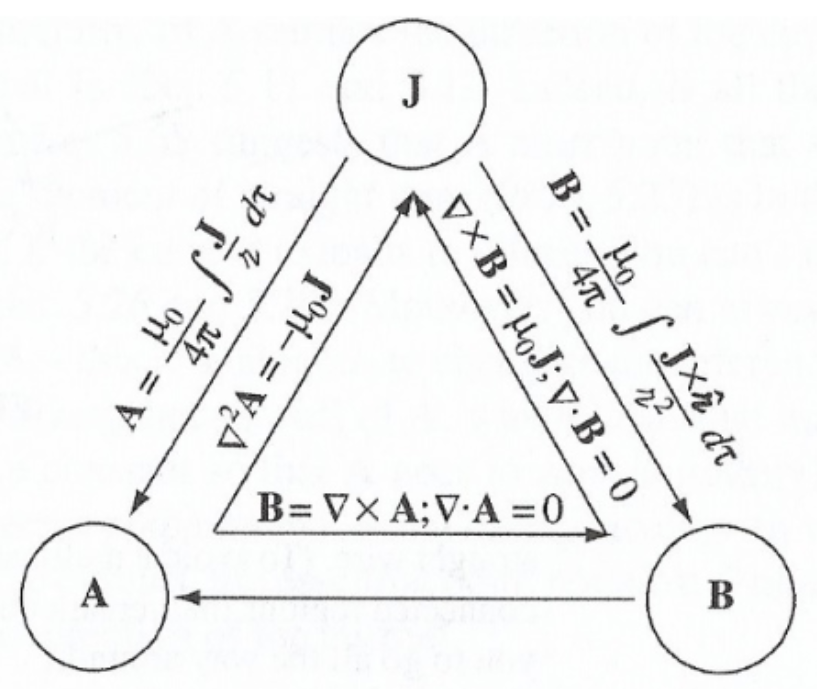
\includegraphics[scale=0.39]{JBA.png}
\end{center}

\newpage
\subsection*{Coulomb Gauge}
Finding a coulomb gauge for a vector potential is always possible, as we can show in the following:
\begin{proof}
Suppose $\vec{A}_0$ is the original vector potential, but it does not satisfy the Coulomb gauge, that is, suppose $\nabla \cdot \vec{A}_0 \neq 0$. We want to find $\vec{A} = \vec{A}_0 + \nabla \Psi$ such that $\nabla \cdot \vec{A} = 0$. Since we require $\nabla \vec{A} = 0 $, then we obtain the following:
\begin{align*}
\nabla^2 \Psi -\nabla \cdot \vec{A}_0
\tag{PA}
\end{align*}
Note that equation (PA) is a Poisson equation. Then for a localized configuration, that is, $\nabla \cdot \vec{A}_0$ vanishes at infinity, equation (PA) has a unique solution given by the following:
\begin{align*}
\Psi(\vec{r}) = \frac{1}{4\pi} \int_V \frac{\nabla' \cdot \vec{A}_0(\vec{r}')}{|\vec{r} - \vec{r}'|}\, d\tau'
\end{align*}
here the operator $\nabla'$ acts on the variable $\vec{r}'$, and $V$ is the localized configuration.
\end{proof}
\hfill\break


\newpage
\subsection*{Magnetic field and Electric field}
Just like in the electrostatic case, the current distribution $\vec{J}$, the magnetic field $\vec{B}$, and the vector potential $\vec{A}$ all give the same information. One can be derived from others though the mathematics involved may be non-trivial. However, because of the vector nature of the potential, it is almost as complicated to calculate as the field. Therefore, it is not as useful as the scalar potential in the electrostatic case.\\

In regions without currents, both the divergence and the curl of the magnetic field vanish:\begin{align*}
\nabla \cdot \vec{B} = 0\qquad\qquad\qquad\qquad \nabla \times \vec{B} = 0
\end{align*}
which is identical to that of the electric field in regions without charges:
\begin{align*}
\nabla \cdot \vec{E} = 0\qquad\qquad\qquad\qquad \nabla \times \vec{E} = 0
\end{align*}
Naturally, one wonders if some of the tools developed for electric field apply here. In deed, in simply connected current-free regions, a scalar potential $V_B$ can be defined for magnetic field as well:
\begin{align*}
\vec{B} = -\nabla V_B \qquad\qquad\Rightarrow\qquad\qquad \nabla^2 V_B = 0
\end{align*}
In this case, some of the tools developed early in Chapter 3 can be applied as well. However, the potential $V_B$ here should be viewed as a mathematical tool, not as a physical quantity.\\

\begin{center}
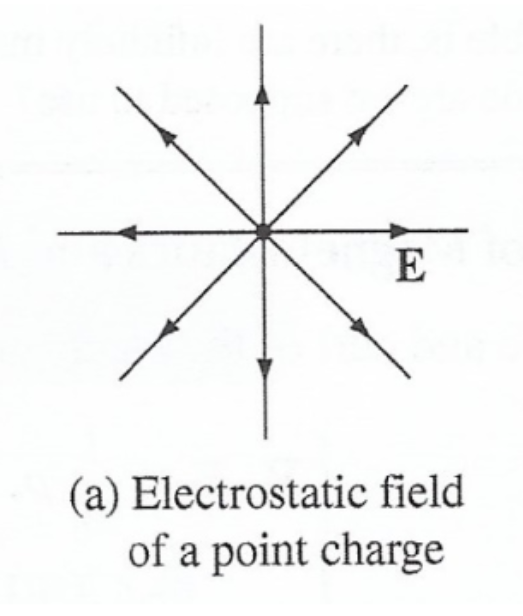
\includegraphics[scale=0.25]{EvsM.png}\qquad\qquad\qquad\qquad\qquad
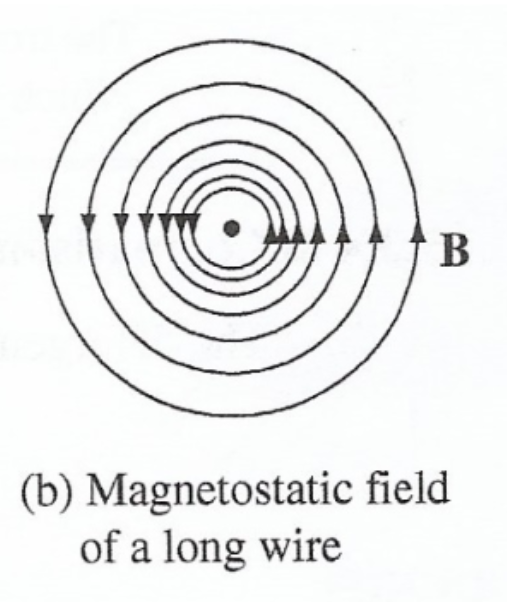
\includegraphics[scale=0.25]{EvsM-Copy.png}
\end{center}

In electrostatics and magnetostatics, static electric and static magnetic fields have very different properties as dictated by divergence and curl properties:
\begin{align*}
\begin{cases}
\nabla \cdot \vec{E} = \frac{\rho}{\epsilon_0} &\text{(Gauss's Law)}\\
\nabla \times \vec{E} = 0\\
\vec{E} = -\nabla V 
\end{cases} \qquad\qquad\qquad\qquad\qquad
\begin{cases}
\nabla \cdot \vec{B} = 0 \\
\nabla \times \vec{B} = \mu_0 \vec{J} &\text{(Ampere's Law)} \\
\vec{B} = \nabla \times \vec{A}
\end{cases}
\end{align*}
Charges produce electric  fields. Electric field lines terminate on charges, diverging from positive charges and converging on negative charges, they never form closed loop.\\

Currents produce magnetic fields. Magnetic field lines curl around currents, they never  terminate. There are no magnetic counterpart of electric charge, the magnetic charge or magnetic monopole.\\

\newpage
\section[Boundary Conditions]{\color{red}Boundary Conditions\color{black}}
Of any closed surface $S$ and closed loop $L$, similar to the electrostatic cases, the integral identities:
\begin{align*}
\oint_S \vec{B}\cdot d\vec{a} = 0 \qquad	\qquad \qquad \oint_L \vec{B}\cdot d\vec{l} = \mu_0 I_{\text{enc}}
\end{align*}
give a set of boundary conditions across surfaces. 

\begin{center}
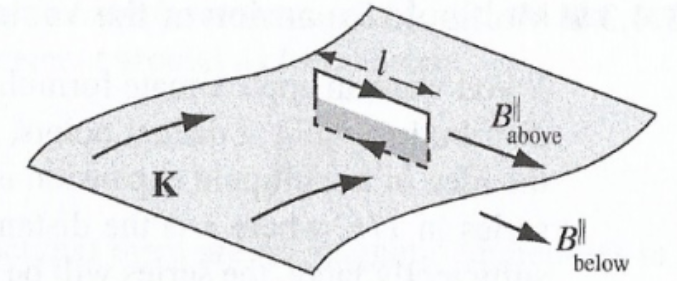
\includegraphics[scale=0.32]{Bpara.png}\qquad\qquad\quad
\includegraphics[scale=0.32]{Bperp.png}
\end{center}


Over a wafer-thin pillbox $S$ straddling the surface of currents, we can write:
\begin{align*}
\oint_S \vec{B}\cdot d\vec{a} = 0 \qquad \qquad \Rightarrow \qquad \qquad B_{\perp}^{above} = B_{\perp}^{below}
\end{align*}
That is, the perpendicular component of the magnetic fields right above and below the surface are the same. In other words, the perpendicular component of the magnetic field is continuous. Over a Amperian loop $L$ running perpendicular to the current, and straddling the surface, we can write:
\begin{align*}
\oint_L \vec{B}\cdot d\vec{l} = (B_{\parallel}^{above} - B_{\parallel}^{below}) l = \mu_0 l k \qquad \Rightarrow \qquad B_{\parallel}^{above} - B_{\parallel}^{below} = \mu_0 K
\end{align*}
where $K$ is the magnitude of the surface current density. That is, the parallel component of the magnetic fields above and below the surface do not agree each other, which suggests the parallel component of the magnetic field that is perpendicular to the current direction discontinuous at a surface current.  A similar Amperian loop running parallel to the current reveals that the parallel component parallel to the current direction is continuous.\\

The boundary conditions for the three components of the magnetic field above and below the surface current can be expressed as the following:
\begin{align*}
\vec{B}^{above} - \vec{B}^{below} = \mu_0 \vec{K}\times \vec{n}
\end{align*}
where $\vec{n}$ is the unit vector normal to the surface pointing upward.\\

For vector potential $\vec{A}$, $\vec{B} = \nabla \times \vec{A}$, requires $\vec{A}$ to be continuous for a finite field, that is, above and below the surface current:
$$\vec{A}^{above} = \vec{A}^{below}$$
while the normal derivative of $\vec{A}$ inherits the discontinuity of $\vec{B}$:
\begin{align*}
\vec{n}\times (\nabla \times \vec{A}^{above} - \nabla \times \vec{A}^{below}) = \mu_0 \vec{n}\times (\vec{K}\times \vec{n}) = \mu_0 \vec{K} 
\end{align*}
\begin{align*}
\left(\frac{\partial \vec{A}}{\partial n} \right)^{above} - \left(\frac{\partial \vec{A}}{\partial n} \right)^{below} = -\mu_0 \vec{K} 
\end{align*}

\newpage
\section[Multipole Expansions]{\color{red} Multipole Expansions\color{black}}
From previous discussion, we can write the magnetic vector potential as the following:
\begin{align*}
\vec{A}(\vec{r}) = \frac{\mu_0 I}{4\pi}\oint_L \frac{d\vec{l}'}{|\vec{r} - \vec{r}'|} = \frac{\mu_0 I}{4\pi}\sum_{n=1}^\infty \frac{1}{r^{n+1}}\oint_L (r')^n P_n(\cos(\alpha)) d\vec{l}'
\end{align*}
with $L$ being the current carrying object.
\begin{center}
\includegraphics[scale=0.3]{BSlaw.png}
\end{center}
Note that we applied the expansion:
\begin{align*}
\frac{1}{|\vec{r}-\vec{r}'|} = \frac{1}{\sqrt{r^2 + (r')^2 - 2rr' \cos(\alpha)}} = \begin{cases}
\frac{1}{r}\sum_{n=0}^\infty \left( \frac{r'}{r}\right)^n P_n (\cos(\alpha)) & r>r'\\
\frac{1}{r'}\sum_{n=0}^\infty \left( \frac{r}{r'}\right)^n P_n (\cos(\alpha)) & r'>r
\end{cases}
\end{align*}
The monopole term, with $n = 0$, is given by the following:
\begin{align*}
\vec{A}_{mon}(\vec{r}) = \frac{\mu_0 I}{4\pi}\oint_L \frac{1}{r}\,d\vec{l}' = 0
\end{align*}
Hence we see that there is no magnetic monopole, that is, there is no magnetic charge.\\

The dipole term, with $n=1$, is given by the following:
\begin{align*}
\vec{A}_{dip}(\vec{r}) = \frac{\mu_0 I}{4\pi} \frac{1}{r^2}\oint_L (r'\cos(\alpha)) \, d\vec{l}' = \frac{\mu_0 I}{4\pi}\frac{1}{r^2}\oint_L( \vec{r}' \cdot \hat{r})\, d\vec{l}'
\end{align*}
Here we note that we can write:
\begin{align*}
\oint_L(\vec{r}'\cdot \hat{r}) d\vec{l}' = -\hat{r}\times \int_S d\vec{a}' = -\hat{r} \times \vec{a}
\end{align*}
where $S$ is any surface enclosed by the loop $L$ and $\vec{a}$ is the vector area of surface $S$.\\
Therefore the dipole term of the vector potential is given by:
\begin{align*}
\vec{A}_{dip}(\vec{r}) = \frac{\mu_0}{4\pi}\frac{\vec{m}\times \hat{r}}{r^2} \qquad\qquad\qquad \text{with }\vec{m} = I \int_S d\vec{a} = I \vec{a}
\end{align*}
where we define $\vec{m}$ to be the magnetic dipole moment, and $\vec{a}$ is the vector area of the current loop defined by:
\begin{align*}
\vec{a} = \frac{1}{2}\oint_L \vec{r}' \times d\vec{l}'
\end{align*}
\newpage

\section[Magnetic Dipole]{\color{red}Magnetic Dipole\color{black}}

For a magnetic dipole placed at the origin with $\vec{m}$ pointing in the positive $z$-direction, we can write:
\begin{align*}
\vec{A}_{dip}(\vec{r}) = \frac{\mu_0}{4\pi}\frac{\vec{m}\times \hat{r}}{r^2} = \frac{\mu_0}{4\pi}\frac{m \, \sin(\theta)}{r^2}\, \hat{\phi}
\end{align*}
The magnetic field is then given by the following:
\begin{align*}
\vec{B}_{dip}(\vec{r}) = \nabla \times \vec{A}_{dip}(\vec{r}) = \frac{\mu_0}{4\pi}\frac{1}{r^3}\left( 3(\vec{m}\cdot \hat{r}) \hat{r} - \vec{m}\right) = \frac{\mu_0}{4\pi}\frac{m}{r^3} \left( 2\cos(\theta)\, \hat{r}+\sin(\theta) \, \hat{\theta}\right)
\end{align*}
Note that the magnetic field has an identical form as the electric field of an electric dipole. 
\begin{center}
\includegraphics[scale=0.65]{Mdipole.png}
\end{center}


\subsection*{Physical and Ideal Dipoles}
For an ideal dipole, or called the pure dipole, the dipole term is the only term in the multipole expansion of the magnetic vector potential:
\begin{align*}
\vec{A}(\vec{r}) = \vec{A}_{dip}(\vec{r}) = \frac{\mu_0}{4\pi}\frac{\vec{m}\times \hat{r}}{r^2}
\end{align*}
For a physical dipole, the dipole term dominates the multipole expansion, with additional contributions from higher-order terms:
\begin{align*}
\vec{A}(\vec{r}) = \frac{\mu_0}{4\pi}\frac{\vec{m}\times \vec{r}}{r^2} + \text{higher-order terms}
\end{align*}
A current loop with a finite size is a physical dipole. As its size shrinks to zero, the higher-order terms in the multipole expansion vanish, and the dipole becomes a pure dipole. Thus a pure dipole is a current loop without physical size.\\
\begin{center}
\includegraphics[scale=0.33]{Mdipole_phy.png}
\end{center}
\newpage

\subsection*{Magnetic Dipole Moments}
For a line current loop $L$, the magnetic dipole moment is given by the following:
\begin{align*}
\vec{m} = I \int_S d\vec{a} = I\vec{a}
\end{align*}
where $S$ is a surface enclosed by the current loop, in which case we can write:
\begin{align*}
\vec{a} = \int_S d\vec{a} = \frac{1}{2}\oint_L \vec{r}\times d\vec{l}
\end{align*}
where $\vec{r} = (x,y,z)$. Thus the dipole moment of a current loop is given by the following:
\begin{align*}
\vec{m} = \frac{1}{2}\oint_L \vec{r}\times d\vec{l} = \frac{1}{2}\oint_L \vec{r}\times \vec{I}
\, dl
\end{align*}
One can extend the definition to surface current $S$ and volume currents $V$:
\begin{align*}
\vec{m} = \frac{1}{2}\int_S \vec{r}\times \vec{K}\, da \qquad\qquad\qquad\qquad \vec{m} = \frac{1}{2}\int_V \vec{r}\times \vec{J}\,d\tau
\end{align*}


\subsection*{Magnetic Dipole in a Magnetic Field}
Consider the following configuration:
\begin{center}
\includegraphics[scale=0.30]{Mtorque.png}
\end{center}
The torque on a small current segment is given by:
\begin{align*}
d\vec{N} = \vec{r} \times d\vec{F} = \vec{r}\times (I d\vec{l}\times \vec{B}) = I \left( ( \vec{r}\cdot \vec{B}) d\vec{l} - (\vec{r}\cdot d \vec{l}) \vec{B}\right)
\end{align*}
Thus the total torque on a current loop $L$ is given by the following:
\begin{align*}
\vec{N} = I \oint_L \vec{r}\times (d\vec{l}\times \vec{B}) = I \oint_L ( \vec{r}\cdot \vec{B})\, d\vec{l} - I \oint_L ( \vec{r} \cdot d\vec{l}) \vec{B}
\end{align*}
For a pure dipole, the field $\vec{B}$ could be considered as a constant vector when evaluating the torque because the pure dipole can be considered as a loop of infinitesimal size. Then we can write:
\begin{align*}
 \oint_L (\vec{r}\cdot \vec{B}) \, d\vec{l} = \vec{a}\times \vec{B} \qquad\qquad\qquad \oint_L \vec{r}\cdot d\vec{l} = \int_S \nabla \times \vec{r}\cdot d\vec{a} = 0
\end{align*}
where $S$ is the surface enclosed by loop $L$, and we have $\vec{m} = I\vec{a}$, hence it follows that the torque about the center of a pure magnetic dipole in non-uniform field, or the torque on a dipole in a constant magnetic field, is given by the following:
\begin{align*}
\vec{N} = I\vec{a}\times \vec{B} = \vec{m} \times \vec{B}
\end{align*}
This shows that the torque tends to rotate the dipole moment along the magnetic field direction. \\

To rotate a pure dipole in non-uniform magnetic field, or a dipole in a constant magnetic field, by an angle $d\theta$, work needs to be done to overcome the torque is given by the following:
\begin{align*}
dW = N d\theta = |\vec{m}\times \vec{B} | d\theta = mB \sin(\theta) d\theta
\end{align*}
Thus the total work to orient the dipole from $\theta_0 = 0$ to the final angle $\theta$ is given by:
\begin{align*}
W = \int_0^{\theta} mB\sin(\theta') d\theta' = mB(1-\cos(\theta))
\end{align*}
This work turns into the potential energy of the dipole in the field.\\

Dropping the irrelevant constant term, the potential energy $U$ of a pure magnetic dipole in a non-uniform field, or a dipole  in a constant magnetic field, is given by:
\begin{align*}
U = -mB\cos(\theta) = -\vec{m}\cdot \vec{B}
\end{align*}

The force on a magnetic dipole is:
\begin{align*}
\vec{F} = I \oint_L d\vec{l}\times \vec{B} = I \oint_L (d\vec{a}\times \nabla)\times \vec{B} = I \oint_L \left( \nabla \left(d\vec{a}\cdot \vec{B}\right) - \left(\nabla \cdot \vec{B}\right) d\vec{a} \right)  = I\oint_L \nabla\left( d\vec{a}\cdot \vec{B}\right) = \nabla \left(\vec{m}\cdot \vec{B}\right)
\end{align*}
hence we see that the force is nonzero only in a nonuniform field.\\

The force, torque, and potential energy of a pure magnetic dipole in nonuniform field, or a dipole in a constant field,  are given by the following:
\begin{align*}
\vec{N} = \vec{m}\times \vec{B} \qquad \qquad U = -\vec{m}\cdot \vec{B} \qquad \qquad \vec{F} = -\nabla U
\end{align*}

\subsection*{Dipole-Dipole Interaction}
From discussion above, it follows that the dipole-dipole interaction potential energy is given by:
\begin{align*}
U = \frac{\mu_0}{4\pi}\frac{1}{r^3}\left( \vec{m}_1 \cdot \vec{m}_2 - 3(\vec{m}_1 \cdot \hat{r})(\vec{m}_2 \cdot \hat{r})\right)
\end{align*}
where $\vec{m}_1,\vec{m}_2$ are the dipole moments of the dipoles, $\vec{r}$ is the distance between the two dipoles. \\
\begin{center}
\includegraphics[scale=0.18]{DipMInt.png}
\end{center}

In particular, we have the followings for dipole-dipole interaction:
\begin{align*}
U_{min} = -\frac{\mu_0}{4\pi} \frac{2m_1m_2}{r^3} \qquad\qquad \qquad \text{when }\vec{m}_1 \text{ is parallel to } \vec{m}_2
\end{align*}
\begin{align*}
U_{max} = \frac{\mu_0}{4\pi} \frac{2m_1m_2}{r^3}\qquad\qquad\qquad \text{when }\vec{m}_1 \text{ is antiparallel to } \vec{m}_2
\end{align*}
Note that there is a symmetry between an electric dipole in an electric field and a magnetic dipole in a magnetic field:
\begin{align*}
\vec{N} = \vec{p}\times \vec{E} \qquad\qquad \qquad U = - \vec{p}\cdot \vec{E}
\end{align*}
\newpage
\section[Electron Magnetic Dipole Moment]{\color{red}Electron Magnetic Dipole Moment\color{black}}
\subsection*{Orbital Magnetic Moment}
Electrons revolve around nuclei. Modeling the motion as a circular motion, the electron has an angular momentum given by:
\begin{align*}
\vec{r}\times \vec{p} = m_e \nu R \hat{z}
\end{align*}
where $m_e$ is the mass of the electron, $\nu$ is the tangential speed of the electron, and $R$ is the radius of the orbit. Modeling the current as a steady current, the electron has an orbital magnetic dipole moment given by the following:
\begin{align*}
\vec{m} = I\vec{a} = \frac{-e}{T}(\pi R^2)\hat{z} = =\frac{e}{2\pi R/\nu}(\pi R^2)\hat{z} = \frac{1}{2}e\nu R\hat{z} = -\frac{e}{2m_e}(m_e \nu R\hat{z}) = -\frac{e}{2m_e}\vec{L}
\end{align*}

\subsection*{Spin Magnetic Moment}
Electrons have intrinsic angular momentum called spin $\vec{S}$, associated with it is the magnetic dipole moment given by the following:
\begin{align*}
\vec{m}_s = g \frac{-e}{2m_e}\vec{S}
\end{align*}
where $g$ is a dimensionless constant called the $g$-factor, here $g= 2$ for electrons.,Deviation from $2$ os called anomalolus magnetic moment.\\

\note In subatomic physics, the magnetic dipole moment $\vec{m}$ is often denoted as $\vec{\mu}$. 

\subsection*{Bohr Magneton}
Both orbital and spin angular momenta are quantized in the unit of $\hbar$, thus the magnetic moment is often expressed in terms of Bohr magneton defined as the following:
\begin{align*}
\mu_B = \frac{e\hbar}{2m_e} = 9.274\cdot 10^{-24}\, J/T
\end{align*}

\newpage
\chapter{Magnetic Fields in Matters}
Because electrons inside materials have both intrinsic and motional magnetic dipole moments, materials will be magnetized in magnetic fields, similar to the polarization in electric fields.\\

Like the Polarization $\vec{P}$, the degree of magnetization is quantified using a quantity called the    the Magnetization $\vec{M}$. $\vec{M}$ is defined to be the magnetic dipole moment per unit volume.\\

While the polarization is almost always in the same direction as $\vec{E}$, this is not the case for the magnetization. Based on their magnetizations, materials can be divided into three groups:
\begin{enumerate}
\item Paramagnetic \,- The magnetization of the material is parallel to $\vec{B}$.
\item Diamagnetic \ \ - The magnetization of the object is in opposite direction to $\vec{B}$
\item Ferromagnetic - The magnetization of the material remain after external $\vec{B}$ is removed.
\end{enumerate}

Paramagnetic materials are made of atoms, or molecules, with odd numbers of electrons. The unpaired electrons give the atoms, or molecules, the intrinsic magnetic moments. These dipoles are usually randomly oriented and therefore cancel each other. However, in an external magnetic field, they tend to align with the field due to the torque, resulting in net macroscopic magnetic moment in the direction of the magnetic field.\\

Diamagnetic materials are made of atoms, or molecules, with even numbers of electrons. The atoms, or molecules, do not have intrinsic magnetic moments as electron pairs have opposite spin and angular momenta. Nevertheless, they acquire magnetic moments from the impacts of the field on their orbits. It is a secondary effect, thus the diamagnetism is generally weaker than the paramagnetism.\\

\subsection*{Mechanism for Diamagnetism}
Circular orbital motion of an electron leads to orbital dipole moment given by the following:
\begin{align*}
\vec{m} = -\frac{e}{2m_e}\vec{L} = -\frac{1}{2}e\nu R\hat{z}
\end{align*}
where $\nu$ is the tangential speed of the electron, $m_e$ is the mass of the electron.\\
\begin{center}
\includegraphics[scale=0.19]{diamag.png}
\end{center}


Such circular centripetal motion is sustained by the Coulomb's fore:
\begin{align*}
\frac{1}{4\pi \epsilon_0}\frac{e^2}{R^2} = m_e\frac{\nu^2}{R}
\end{align*}
In a magnetic field $\vec{B}$, the electron will also experience a magnetic force $\vec{F}_m = -e(\vec{\nu}\times \vec{B})$, an additional centripetal force, which could speed up or slow down the electron. If $\vec{B}$ is perpendicular to the orbit, then we can write the following, with $\bar{\nu}$ denoting the tangential speed of the electron under the influence of the magnetic field, and $\nu$ denoting the tangential speed of the electron without the magnetic field:
\begin{align*}
\frac{1}{4\pi \epsilon_0}\frac{e^2}{R^2} + e\bar{\nu}B = m_e \frac{\bar{\nu}^2}{R} \qquad \Rightarrow \qquad e\bar{\nu}B = m_e \frac{\bar{\nu}^2}{R} - m_e \frac{\nu^2}{R} = \frac{m_e}{R}(\bar{\nu}+\nu)(\bar{\nu}-{\nu})
\end{align*}
The change in speed $\Delta \nu$ and the resulting change in dipole moment $\Delta \vec{m}$ are then given by the following:
\begin{align*}
\Delta \nu = \bar{\nu} - \nu = \frac{eBR}{m_e}\frac{\bar{\nu}}{\bar{\nu} - \nu} \approx \frac{eBR}{2m_e}\qquad\qquad\qquad \Delta \vec{m} = -\frac{1}{2}eR\Delta\nu \hat{z} \approx -\frac{e^2R^2}{4m_e}\vec{B}
\end{align*}
Note that $\Delta \vec{m}$ is proportional to $\vec{B}$, but in opposite direction. This is true even if $\vec{B}$ points in opposite direction, or the electron moves in the opposite direction.\\

In a magnetic field, each atom pickup a small extra dipole moment that is anti-parallel to the field. This is the mechanism responsible for diamagnetism. It is a universal phenomenon, but is typically much weaker than paramagnetism, and it is observed mainly in atoms with even numbers of electrons.\\
\newpage
\section[Magnetic Field of Magnetized Object]{\color{red} Magnetic Field of Magnetized Object \color{black}}
The potential of a dipole at the origin is given by:
\begin{align*}
\vec{A}_{dip}(\vec{r}) = \frac{\mu_0 (\vec{m}\times \hat{r})}{4\pi r^2} = \frac{\mu_0}{4\pi}\frac{\vec{m}\times \vec{r}}{r^3}
\end{align*}
Thus the vector potential at $\vec{r}$ due to an infinitesimal dipole $d\vec{m}$ at $\vec{r}'$ is given by:
$$d\vec{A}(\vec{r}) = \frac{\mu_0}{4\pi}(d\vec{m})\times \frac{\vec{r} - \vec{r}'}{|\vec{r}-\vec{r}'|^3}$$
\begin{center}
\includegraphics[scale=0.19]{MfielfMagObj.png}
\end{center}
and hence the vector potential at $\vec{r}$ due to a magnetized object $V$ is given by the following:
\begin{align*}
\vec{A}(\vec{r}) = \frac{\mu_0}{4\pi}\int_V(d\vec{m})\times \left(\frac{\vec{r}-\vec{r}'}{|\vec{r}-\vec{r}'|^3} \right) = \frac{\mu_0}{4\pi}\int_V (\vec{M}(\vec{r}'))\times  \left(\frac{\vec{r}-\vec{r}'}{|\vec{r}-\vec{r}'|^3} \right) \, d\tau' \tag{AD}
\end{align*}
Note that we have the followings, with $\nabla'$ operating on $\vec{r}'$:
\begin{align*}
\nabla'\left(\frac{1}{|\vec{r}-\vec{r}'|}\right) = \frac{\vec{r} - \vec{r}'}{|\vec{r}- \vec{r}'|^3}
\end{align*}
then we can rewrite equation (AD) as the following:
\begin{align*}
\vec{A}(\vec{r}) = \frac{\mu_0}{4\pi}\int_V (\vec{M}(\vec{r}')) \times\left( \nabla'\left(\frac{1}{|\vec{r}-\vec{r}'|}\right) \right) \, d\tau' = \frac{\mu_0}{4\pi}\int_V \left( \frac{\nabla' \times \vec{M}(\vec{r}')}{|\vec{r}-\vec{r}'|} - \nabla' \times \left(\frac{\vec{M}(\vec{r}')}{|\vec{r}-\vec{r}'|}\right)\right) \, d\tau' \tag{MD}
\end{align*}
By divergence theorem, let $S$ be the boundary of $V$, the second integral in equation (MD) has the following form:
\begin{align*}
\int_V \nabla' \times \left(\frac{\vec{M}(\vec{r}')}{|\vec{r}-\vec{r}'|}\right) \, d\tau' = \oint_S \frac{d\vec{a}\times \vec{M}(\vec{r}')}{|\vec{r}-\vec{r}'|} = -\oint_S \frac{\vec{M}(\vec{r}')\times \vec{n}}{|\vec{r}-\vec{r}'|}\, da'
\end{align*}
Putting altogether, we get the following vector potential:
\begin{align*}
\vec{A}(\vec{r}) =\left( \frac{\mu_0}{4\pi}\int_V \frac{\vec{J_b(\vec{r}')}}{|\vec{r}-\vec{r}'|}\, d\tau' \right)\ +\ \left( \frac{\mu_0}{4\pi}\oint_S \frac{\vec{K}_b(\vec{r}')}{|\vec{r}-\vec{r}'|}\, da'\right) 
\end{align*}
where we define:
\begin{align*}
\vec{J}_b \coloneqq \nabla \times \vec{M} \qquad\qquad\qquad\qquad\qquad \vec{K}_b \coloneqq \vec{M}\times \vec{n}
\end{align*}
\note The potential due to a magnetized object with magnetization $\vec{M}$ is the same as that produced by a volume current $\vec{J}_b = \nabla \times \vec{M}$, and by a surface current $\vec{K}_b = \vec{M}\times \vec{n}$. These magnetization induced currents are called the bound currents. \\



\subsection*{Field of Uniformly Magnetized Objects}
One can easily show that there are no volume bound current inside uniformly magnetized objects, but in general, there will be bound surface currents on such object.\\

\example\\
For a long cylinder oriented aligned with the $z$-axis, and with magnetization $\vec{M}$ pointing in the positive $z$-direction, we have $\vec{K}_b = \vec{M}\times \vec{n} = M \, \hat{\phi}$, this is similar to a long solenoid, thus the magnetic field produced by such magnetization is given by the following:
\begin{align*}
\vec{B} = \begin{cases} \mu_0 \vec{M} & \text{ inside the cylinder}\\
0 & \text{ outside the cylinder}
\end{cases}
\end{align*}
\hfill\break\hfill\break
\example\\
For a thin wafer oriented aligned with the $z$-axis, and with magnetization $\vec{M}$ pointing in the positive $z$-direction, we still have $\vec{K}_b = M \, \hat{\phi}$. For a wafer with its thickness much smaller than its cross sectional dimension, the field produced by this current is negligible. \\
\hfill\break
Bound currents are due to the alignments of magnetic moments. After done rigorous mathematical derivation, here are heuristic arguments, similar to those of bound charges. For a uniformly magnetized object, the currents of internal dipoles cancel each other, leaving net currents on the surfaces. Similarly, if the magnetization is not uniform, the currents of internal dipoles will not cancel, results in volume bound currents.
\begin{center}
\includegraphics[scale=0.35]{bddCurrents.png}
\end{center}

For conductor inside a magnetic field, unlike in the electrostatic case, the magnetic field can live inside a conductor. Electrons will move because of the magnetic force. But the motion is random because of random electron velocity. Thus there will not be induced currents to produce magnetic field that cancel exactly the external field. This is not the case in electric case in which the force is opposite to the electric field. However, superconductors expel magnetic field, that is, the magnetic field inside
vanishes, but that is a quantum mechanical effect. \\

\newpage
\section[Ampere's Law in Magnetized Materials]{\color{red}Ampere's Law in Magnetized Materials\color{black}}
In the presence of magnetized objects objects that carry free currents, we have two types of currents, (1) the free current, denoted as $\vec{J}_f$, due to the movement of charges, and (2) the bound current $\vec{J}_b$, due to the magnetization of the object.\\

The total current density is the sum of the two, given by the following:
\begin{align*}
\vec{J} =\vec{J}_f + \vec{J}_b
\end{align*}
The Ampere's Law now can be written as the following:
\begin{align*}
\nabla \times \vec{B} = \mu_0 \vec{J} = \mu_0 (\vec{J}_f + \vec{J}_b) \qquad \Rightarrow \qquad \nabla \times \left( \frac{\vec{B}}{\mu_0} - \vec{M}\right) = \vec{J}_f
\end{align*}
Here we define a new field called the auxiliary field $\vec{H} $ as the following:
\begin{align*}
\vec{H}\coloneqq \frac{\vec{B}}{\mu_0} - \vec{M}
\end{align*}
The Ampere's Law now reads:
\begin{align*}
\nabla \times \vec{H} = \vec{J}_f \qquad \Rightarrow \qquad \oint_L \vec{H}\cdot d\vec{l} = I_{f, \text{ enc}}
\end{align*}
where $L$ is an arbitrary loop, and $I_{f, \text{ enc}}$ denote the free current enclosed by the loop $L$. In regions without free current, we have $\nabla \times \vec{H} = 0$.\\

\remark The magnetic field $\vec{B}$ is determined by both the free and bound currents while the auxiliary field $\vec{H}$ is determined by the free current only. The free current is what we control, thus $\vec{H}$ is a more useful quantity than $\vec{B}$ for electromagnets. For this region, $\vec{H}$ is called the magnetic field and $\vec{B}$ is called the magnetic induction in some literatures.\\

On the other hand, $\vec{D}$ is not that useful in electrostatic case even though it is determined by the free charge. This is because the voltage is controllable and the voltage is directly related to the electric field $\vec{E}$, while the free charge is much harder to be controlled in this sense.  


\newpage
\section[Linear Magnetic Media]{\color{red}Linear Magnetic Media\color{black}}
For most substances, the magnetization is proportional to the field as long as it is not too strong. The proportionality is expressed as the following:
\begin{align*}
\vec{M} = \chi_m \vec{H}
\end{align*}
The dimension-less constant $\chi_m$ is a material property called the magnetic susceptibility. Materials with this property are called the linear magnetic media. \\

For must materials, $\chi_m$ is small. Unlike $\chi_e$, $\chi_m$ can be both positive and negative. For linear media with $\chi_m>0$, the media is paramagnetic, and for linear media with $\chi_m<0$, the media is diamagnetic.\\

For linear media, we can write the following:
\begin{align*}
\vec{B} = \mu_0 (\vec{H}+\vec{M}) = \mu_0 ( 1+\chi_m )\vec{H} \coloneqq \mu \vec{H} \qquad \Rightarrow \qquad \vec{B} = \mu \vec{H}
\end{align*}
with $\mu\coloneqq \mu_0(1+\chi_m)$ being the permeability of the linear magnetic material. \\
We have $\mu \approx \mu_0$ for most materials except for ferromagnets. \\

\note The bound and free current densities are proportional in a linear material:
\begin{align*}
\vec{J}_b = \nabla \times \vec{M} = \nabla \times (\chi_m \vec{H}) = \chi_m \nabla \times \vec{H} = \chi_m \vec{J}_f \qquad \Rightarrow \qquad \vec{J}_b = \chi_m \vec{J}_f
\end{align*}
\note Even though we have $\vec{B} = \mu \vec{H}$ in a linear medium and $\nabla \cdot \vec{B} = 0$, we generally have $\nabla \cdot \vec{H}\neq 0$ around the medium boundaries. 

\newpage
\section[Boundary Conditions]{\color{red}Boundary Conditions\color{black}}
The boundary conditions for $\vec{B}$ still hold at boundaries $S$ of magnetized materials:
\begin{align*}
\oint_S \vec{B}\cdot d\vec{a} = 0 \qquad \Rightarrow \qquad B_{\perp}^{above}-B_{\perp}^{below} = 0 \qquad \Rightarrow \qquad \vec{n}\cdot (\vec{B}^{above} - \vec{B}^{below}) = 0
\end{align*}
Let $L$ be an arbitrary closed loop on the boundaries of the material:
\begin{align*}
\oint_L \vec{B}\cdot d\vec{l} = \mu_0 I_{\text{enc}} \qquad \Rightarrow \qquad \vec{B}^{above} - \vec{B}^{below} = \mu_0(\vec{K}\times \vec{n}) \qquad \Rightarrow \qquad \vec{n}\times (\vec{B}^{above} - \vec{B}^{below}) = \mu_0 \vec{K}
\end{align*}
Here we have $\vec{K} = \vec{K}_f + \vec{K}_b$. \\

The auxiliary field $\vec{H}$ is subjected to the following conditions:
\begin{align*}
\int_S \vec{H}\cdot d\vec{a} = \oint_S \vec{M}\cdot d\vec{a} \qquad \Rightarrow \qquad H_{\perp}^{above} = -(
M_{\perp}^{above} - M_{\perp}^{below} 
\end{align*}
\begin{align*}
\oint_L \vec{H}\cdot d\vec{l} = I_{f, \text{ enc}} \qquad \Rightarrow \qquad (\vec{H}_{\parallel}^{above} - \vec{H}_{\parallel}^{below}) = \vec{K}_f
\times \vec{n}
\end{align*}
Here we get:
\begin{align*}
(\vec{H}_{\parallel}^{above} - \vec{H}_{\parallel}^{below}) = \vec{K}_f
\times \vec{n}
\end{align*}
Note that we also have: 
$$\vec{B} = \nabla \times \vec{A}\qquad \Rightarrow \qquad \vec{A}^{above}  -\vec{A}^{helow}=0$$
and lastly:
\begin{align*}
\vec{n}  \times (\nabla \times \vec{A}^{above} - \nabla \times \vec{A}^{below}) = \mu_0 \vec{K}
\end{align*}


\section[Ferromagnets]{\color{red}Ferromagnets\color{black}}
Ferromagnets are materials that retain their magnetizations even after the external has been removed. The magnetizations are frozen in. These materials have memories and are inherently non-linear. Common ferromagnetic materials are iron, nickel, cobalt and their alloys, and are used to make permanent magnets.\\

\subsection*{Magnetization and Hysteresis Loop}
In a ferromagnet, the magnetization at a time depends not only the external field at the time, but also its history. The magnetization will trace out a loop, called hysteresis loop, when external field is applied or removed.\\

\begin{center}
\includegraphics[scale=0.25]{HysteresisL.png}
\end{center}

The mechanism of ferromagnetism is quantum mechanical. In a nutshell, dipoles do not act individually, they form domains. Within a domain, all dipoles point in the same direction. Domains themselves are randomly oriented. In an external strong magnetic field, these domains tend to align with the field. Domains parallel to the field will also grow by winning over dipoles at the boundaries. If the field is strong enough, one domain can take over entirely. The magnetization is said to be saturated. Random thermal motions will compete with the orderly magnetization. At very high temperatures, they will destroy the alignment. The lowest temperature at which the alignment is destroyed is called Curie point. For iron, it is $770^{\circ}$ C.\\

\section[Magnetic Poles]{\color{red} Magnetic Poles \color{black}}
Magnetic poles are the two ends of a magnet where the magnetic field is strongest. They are named North and South poles. The whole concept is based on magnetic charges, copied from electrostatic case. In this model, called Gilbert model, magnetic field lines originate from the north pole and terminate at the South pole.\\

Similar to electric charges, opposite poles attract and like poles repel.\\

Magnetic north pole is geographic south pole. Magnetic south pole is geographic north pole.\\

\hfill\break
\begin{center}
\includegraphics[scale=0.29]{Mpoles.png}
\end{center}

\newpage
\chapter{Electrodynamics}
\section[Ohm's Law]{\color{red}Ohm's Law\color{black}}
To make a current flow, there must be a force to push the charges. For most substances, the current density $\vec{J}$ is proportional to the force per unit charge $\vec{f}$:
\begin{align*}
\vec{J} = \sigma \vec{f}
\end{align*}
The proportional constant $\sigma$ is a material property, called the conductivity, and is reciprocal to what is called the resistivity:
\begin{align*}
\rho = \frac{1}{\sigma}
\end{align*}
\example\\
For perfect conductors, we have $\rho = 0$, $\sigma = \infty$.\\
For perfect insulators, we have $\rho = \infty$, $\sigma = 0$.\\

If the force pushing the charges is electromagnetic in nature, then we have $\vec{f} = \vec{E} + \vec{v}\times \vec{B}$. In most cases, the magnetic force is small and can be ignored, hence we write:
\begin{align*}
\vec{J} = \sigma \vec{E} \tag{OH}
\end{align*}
Equation (OH) is called the Ohm's Law, which is an empirical law, not a fundamental law of nature.\\

The materials that obey Ohm's Law are called Ohmic materials. \\

\subsection*{Resistivity and conductivity}
For electrostatic case, we have $\vec{J} = 0$ and $\vec{E} = 0$ inside a conductor. However, the electric field is $\vec{E} = \vec{J}/\sigma \approx 0$ inside a good conductor even in non-electrostatic cases.\\

For a steady current, with charge density $\rho$, we can write the following by Gauss's Law and Ohm's Law:
\begin{align*}
\rho = \epsilon_0 \nabla \cdot \vec{E} = \frac{\epsilon_0}{\sigma} \nabla \cdot \vec{J} = 0\qquad\qquad\qquad \nabla \cdot \vec{J}+\frac{\partial \rho}{\partial t} = 0
\end{align*}
there is no charge inside the material, any net charge must reside on the surfaces, which is the same as the electrostatic case.\\

For a segment of a wire with constant cross section, the resistance is given by:
\begin{align*}
R \coloneqq  \frac{\rho L}{A}
\end{align*}
Hence we have:
\begin{align*}
\rho = R = \frac{A}{L} \qquad \qquad \Rightarrow \qquad \qquad \rho = R\frac{A}{L}
\end{align*}
The resistance is defined to have unit $\Omega$, and hence resistivity $\rho$ has SI unit $\Omega\, m$. The conductivity has the unit of $\Omega^{-1}\, m^{-1} \coloneqq S/m$, here $S$ is Siemens, and $1\, S = 1\, \Omega^{-1}$.\\


\begin{thm}[Ohm's Law]
For a cylinder resistor of a constant cross-sectional area $A$ and length $L$, the electric field inside is uniform if a voltage $V$ is applied, and we can write $V = IR$. 
\end{thm}
\begin{center}
\includegraphics[scale=0.25]{ohmLaw.png}
\end{center}

\begin{proof}
The potential obeys Laplace's equation inside the cylinder with the boundary conditions given by: (1) constant potentials at the two ends, assuming that we have $V(z) = 0$ at $z=0$, and $V(z) = V_0$ at $z=L$, and (2) no current flowing out of the side, that is, we have $\vec{J}\cdot \vec{n} = 0 $, and hence we have $\vec{E} \cdot \vec{n}=0$, so we have $\frac{\partial V}{\partial n} = 0$.\\

\begin{center}
\includegraphics[scale=0.25]{ohmLawProof.png}
\end{center}

It is not difficult to guess the solution to the Laplace's equation that meets the boundary conditions in this case:
\begin{align*}
V(z) = \frac{zV_0}{L} \qquad\qquad \Rightarrow \qquad \qquad \vec{E} = -\nabla V = -\frac{V_0}{L}\, \hat{z} \tag{*}
\end{align*}
By the Uniqueness Theorem, equation (*) must gives the right solution, so the electric field inside the conductor is uniform. The electric current is then given by the following:
\begin{align*}
I = JA = \sigma E A = \frac{\sigma AV}{L} \qquad \Rightarrow \qquad I = \frac{V}{R} \qquad \text{with}\ R = \frac{L}{\sigma A} = \frac{\rho L}{A}
\end{align*}
This gives the familiar form of the Ohm's Law, where $R$ is known as the resistance, measured in Ohms in the SI units, and $1\, \Omega = 1\, V/A$. Also note that, over a resistor, the electric potential is given by:
\begin{align*}
\int \vec{E}\cdot d\vec{l} = El = V = IR
\end{align*}
\end{proof}

\subsection*{A Microscopic Model of Ohm's Law}
Electron will accelerate under electric forces, that is, $\nu$ increases, which implies $||\vec{J}||$ increases, and theoretically we should have $I$ increases as a result. However, the current does not increase over time under a given voltage.\\

The answer to this is that electrons have random fast thermal motion and collide frequently with nuclei, resulting in vanishing average velocities. \\

\begin{center}
\includegraphics[scale=0.22]{driftElectron.png}
\end{center}
When an external field $\vec{E}$ is applied, electrons acquire a steady drift velocity along the $\vec{E}$ direction. Let $\lambda$ be the average distance between two successive collisions and let $\left<\nu\right>$ denote the average thermal speed, then the average velocity, or the drift velocity, gained by an electron due to $\vec{E}$ is given by:
\begin{align*}
\vec{\nu}_d = \frac{1}{2}\vec{a}\left< t\right> = \frac{1}{2}\left( \frac{-e\vec{E}}{m_e}\right) \left( \frac{\lambda}{\left< \nu\right>}\right) = \frac{e\lambda}{2m_e\left<\nu\right>}\vec{E}
\end{align*}
Any orderly motion along $\vec{E}$ is destroyed by the collisions since $\left< \nu\right> >>\nu_d$. The current density is then given by the following:
\begin{align*}
\vec{J} = (-n_e e)\vec{\nu}_d  = \frac{n_e e^2 \lambda}{2m_e \left< \nu\right>}\vec{E} = \sigma \vec{E}
\end{align*}
where we define: $$\sigma \coloneqq \frac{n_e e^2 \lambda}{2m_e\left< \nu\right>}$$
and $n_e$ is the density of mobile electrons. As a results of the collisions, the energy is converted into heat, and the power delivered is given by the Joule Heating Law:
\begin{align*}
P = IV = I^2 R
\end{align*}
For kinetic model of ideal gas, we write:
\begin{align*}
\left<\nu \right> = \sqrt{\frac{8k_b T}{\pi m}}\qquad\qquad\qquad \lambda=\frac{k_b T}{4\sqrt{2}\pi r^2 p}
\end{align*}
where $k_b$ is the Boltzmann's constant, and in standard atmospheric pressure, we have $\left< t\right> \approx 10^{-10}\, s$, and $\lambda \approx 10^{-8}\, m$.\\
\newpage


\section[Electromotive Force]{\color{red} Electromotive Force \color{black}}
In a circuit, there are two forces driving the current. The first one is the force of the source in the source, denoted as $\vec{f}_s$, the source can be battery, generator, and so on. The other force is the electrostatic force from the electric field in the circuit, related to $\vec{E}$. $\vec{f}$ drives the current inside the source and $\vec{E}$ drives the current outside the source in the circuit.\\

The total force per unit charge is then given by:
\begin{align*}
\vec{f} = \vec{f}_s +\vec{E}
\end{align*}
the work done by the force in pushing a unit charge through one loop $L$ of a circuit is then given by:
\begin{align*}
\mathcal{E} = \oint_L \vec{f}\cdot d\vec{l} = \oint_L \left( \vec{f}_e + \vec{E}\right) \cdot d\vec{l} = \oint_L \vec{f}_e \cdot d\vec{l} = \oint_L \vec{f}_s \cdot d\vec{l}
\end{align*}
Here $\mathcal{E}$ is called the electromotive force, or emf for short, of the circuit. Note that $\mathcal{E}$ is not a force, instead, $\mathcal{E}$ is the work done per unit charge by the force.\\

Inside a source such as a battery, the electrons move in the opposite direction of the electric force. Thus the source force $\vec{f}_s$, from chemical process or related, has to overcome electric force given by $\vec{E}$, say we have $\vec{f}_e = -\vec{E}$, then the voltage of the battery is given by:
\begin{align*}
V = -\int \vec{E}\, \cdot d\vec{l} = \int \vec{f}\cdot d\vec{l} = \oint_L \vec{f}_s \cdot d\vec{l} = \mathcal{E}
\end{align*}
For a battery, emf gives the voltage of the battery, the work done by the battery in moving a unit charge one trip through the loop is given by the value of emf.\\

\subsection*{Motional emf}
Motional emf arises when a conducting wire is moved through a magnetic field. The magnetic force is the source force. Generators are operated on the motional emfs.\\

Consider a conducting rectangular loop $L$ is pulled to the right. 

\begin{center}
\includegraphics[scale=0.23]{emfloop.png}
\end{center}

There is a magnetic field going through the left half of the loop, perpendicular to the flat surface formed by the loop. The free electrons in segment $ab$ will move, therefore establishing a current in the loop. The emf in this case is given by the following:
\begin{align*}
\mathcal{E} = \oint_L \vec{f}_{m}\cdot d\vec{l} = Bh\nu
\end{align*}
where $\nu$ is the speed that the loop is pulled, and $h$ is the length of segment $ab$. Note that the magnetic flux through the loop is given by the following:
\begin{align*}
\Phi = BA = Bxh \qquad \Rightarrow \qquad \frac{d \Phi}{dt} = -Bh \nu
\end{align*}
Therefore, the emf in this case can be written as the following:
\begin{align*}
\mathcal{E} = -\frac{d\Phi}{dt} \tag{F}
\end{align*}
Equation (F) gives the universal flux rule of emf. Though we derived it for a special case, the flux rule is valid for all sources of the flux change, through uniform or non-uniform field.\\

Whenever the flux through a loop changes for whatever the reason, there will be emf in the circuit which is equal to the time rate of the flux change. The negative sign tells the direction of the current flow due to the emf.\\

\newpage
\section[Faraday's Law of Induction]{\color{red} Faraday's Law of Induction\color{black}}
The Faraday's Law of Induction is named after British scientist Michael Faraday (1791 - 1867). In 1831, Faraday reported the observation of current in a conducting loop, which initially is partially in a magnetic field, and the magnetic field lines goes through the left half of the loop, perpendicular to the surface formed by the loop, from three different experiments:
\begin{enumerate}[topsep=3pt,itemsep=-1ex,partopsep=1ex,parsep=1ex,label=(\alph*)]
\item Pull the conducting loop to the right 
\item Pull the magnetic field to the left 
\item Decrease the magnitude of the magnetic field
\end{enumerate}
\begin{center}
\includegraphics[scale=0.23]{faraday.png}
\end{center}

Moreover the currents flew in the same direction for all three experiments. It is easy to understand that experiment (a) and (b) are the same as the motion is relative. The surprising result is from experiment (c) in which neither the field and the loop are moving. So whatever drives the current cannot be the magnetic force. It is the electric field driving the current in experiment (c), electric field can not only be produced by charges, but can also be induced from the change in magnetic field. That is, a changing magnetic field induces an electric field. \\

\begin{thm}[Faraday's Law of Induction]
Mathematically, the result of such experiment can be summarized by taking $\vec{f}_s =\vec{E}$, in which case we can write the following, with $L$ being the conducting loop:
\begin{align*}
\mathcal{E} = \oint_L \vec{E}\cdot d\vec{l} = -\frac{d\Phi}{dt} = -\frac{d}{dt}\int_S \vec{B}\cdot d\vec{a} \qquad \qquad \Rightarrow \qquad \qquad \int_S \nabla \times \vec{E}\cdot d\vec{a} = -\int_S \left( \frac{\partial \vec{B}}{\partial t}\right) \cdot d\vec{a}
\end{align*}
where $S$ is the surface enclosed by the loop $L$. Thus the integral and differential form of the Faraday's Law read the following:
\begin{align*}
\oint_L \vec{E}\cdot d\vec{l} = -\frac{d}{dt}\int_S \vec{B}\cdot d\vec{a} \qquad\qquad\qquad\qquad\qquad \nabla \times \vec{E} = -\frac{\partial \vec{B}}{\partial t}
\end{align*}
\end{thm}
Faraday's Law reduces to the familiar form for the static case when we have $\frac{\partial \vec{B}}{\partial t} = 0$:
\begin{align*}
\frac{\partial \vec{B}}{\partial t} = 0 \qquad  \Rightarrow  \qquad \oint_L \vec{E}\cdot d\vec{l} = 0 \qquad \Rightarrow \qquad \nabla \times \vec{E} = 0
\end{align*}
Faraday's Law encompasses the static case, but it extends it to the time-dependent case.\\

It is the electric field induced from changing magnetic field that gives rise to the emf in experiment (c). The emfs in all three experiments can be described by the flux rule. Whenever, and for whatever reason, the magnetic flux through a loop changes, an emf will appear in the loop:
\begin{align*}
\mathcal{E} = -\frac{d\Phi}{dt}
\end{align*}

\begin{thm}[Len's Law]
Len's Law was formulated by Russian physicist Emil Lenz in 1834, a few years after the revolutionary development of the induced field. Len's Law states that the electric current induced by a changing magnetic field is in such a direction that the magnetic field it creates opposes the change in the initial magnetic field.
\end{thm}

Lenz's Law is a qualitative statement that specifies the direction of the induced current, it says nothing about the magnitude of the induced current. Len's Law is not a new law, it is the interpretation of the minus sign in the universal flux rule or in the Faraday's Law of induction, but Lenz's Law does offer an easy way to determine the direction of the induced current. \\

\newpage
\section[The Induced Electric Field]{\color{red}The Induced Electric Field\color{black}}
The Faraday's Law specifies the curl of the induced electric field, the divergence is still governed by the Gauss's Law $\nabla \cdot \vec{E} = \rho/\epsilon_0$. If $\vec{E}$ is purely induced due to a changing $\vec{B}$, then we can write:
\begin{align*}
\nabla \cdot \vec{E} = 0 \qquad\qquad\qquad\qquad\qquad \nabla \times \vec{E} = -\frac{\partial \vec{B}}{\partial t}
\end{align*}
Mathematically identical to the magnetostatics expression given by the following:
\begin{align*}
\nabla \cdot \vec{B} = 0 \qquad\qquad\qquad\qquad\qquad \nabla \times \vec{B} = \mu_0 \vec{J}
\end{align*}
The induced electric field is determined by $-\frac{\partial \vec{B}}{\partial t}$, here we can write:
\begin{align*}
\vec{E}(\vec{r}) =- \frac{1}{4\pi}\int \frac{\partial \vec{B}(\vec{r}')}{dt}\times \left( \frac{\vec{r}-\vec{r}'}{|\vec{r}-\vec{r}'|}\right) \, d\tau'
\end{align*}
and the mathematical expression of Faraday's Law is similar to that of Ampere's Law:
\begin{align*}
\oint \vec{E}\cdot d\vec{l} = -\int \frac{\partial \vec{B}}{\partial t} \cdot d\vec{a} = -\frac{d}{dt}\int \vec{B}\cdot d\vec{a} = -\frac{d\Phi}{dt}
\end{align*}

\example\\
The lines of induced $\vec{E}$ form closed loops, curling around $-\frac{\partial \vec{B}}{\partial t}$, just like $\vec{B}$ curling around the current in magnetostatics.

\begin{center}
\includegraphics[scale=0.23]{emf.png}
\end{center}

\subsection*{Induced Vector Potential and Current Density}
One may have noted that we have the following, with $\vec{A}$ being the vector potential of a magnetic field $\vec{B}$:
\begin{align*}
\vec{B} = \nabla \times \vec{A}\qquad\qquad\qquad\qquad \nabla \times \vec{E} = -\frac{\partial \vec{B}}{\partial t}
\end{align*}
Combining we get the following:
\begin{align*}
\nabla \times \vec{E} = -\nabla \times \left( \frac{\partial \vec{A}}{\partial t}\right)\qquad\qquad \Rightarrow \qquad \qquad \nabla \times \left( \vec{E} + \frac{\partial \vec{A}}{\partial t}\right) = 0
\end{align*}
Thus the induced field and the change rate of the vector potential are directly related, they could differ by curl-less function which can be expressed as a gradient of a scalar function:
\begin{align*}
\vec{E}+\frac{\partial \vec{A}}{\partial t} = -\nabla V \qquad \qquad \Rightarrow \qquad\qquad \vec{E} = -\nabla V - \frac{\partial \vec{A}}{\partial t}
\end{align*}
This form of the electric field encompasses both the static and non-static cases. The first term $-\nabla V$ represents the field from static charge distribution, while the second term is the induced field from a changing magnetic field.\\

Taking curl of the Faraday's Law, we get the following:
\begin{align*}
\nabla \times \left(\nabla \times \vec{E}\right) = -\nabla \times \left( \frac{\partial \vec{B}}{\partial t}\right) \qquad \Rightarrow \qquad \nabla\left( \nabla \cdot \vec{E}\right) - \nabla^2 \vec{E} = -\frac{\partial }{\partial t}\left( \nabla \times \vec{B}\right) = -\mu_0 \frac{\partial \vec{J}}{\partial t} 
\end{align*}
Note that $\nabla \cdot \vec{E} = 0$ if the electric field is induced only, in which case we can write the following:
\begin{align*}
\nabla^2 \vec{E} = \mu_0 \frac{\partial \vec{J}}{\partial t}
\end{align*}
Therefore, the induced field from a changing $\vec{B}$ due to a changing volume current $\vec{J}$ is then given by the following:
\begin{align*}
\vec{E}(\vec{r}) = -\frac{\partial \vec{A}(\vec{r})}{\partial t} = -\frac{\mu_0}{4\pi}\int \frac{\partial \vec{J}(\vec{r}')}{\partial t}\frac{d\tau'}{|\vec{r}-\vec{r}'|}
\end{align*}
Note that $\vec{E}$ is in the direction of $-\frac{\partial \vec{J}}{\partial t}$.\\


\subsection*{Eddy Currents}
Eddy currents are electric currents induced within conductors by a changing magnetic field. They flow in closed loops in planes perpendicular to the magnetic field. The term comes from analogous  currents seen in water due to localized turbulence known as eddies.\\

\begin{center}
\includegraphics[scale=0.23]{eddy.png}
\end{center}

Eddy currents are the results of induced emf and the interaction between the eddy currents and the magnetic field will cause a drag force on the moving conductor or magnet. This is the principle of eddy current brakes which work well at high speeds, but not so at low speeds.\\

Eddy currents are nuisances in many other applications. They cause energy losses in inductors, generators, transformer etc. They can be reduced, for example, by laminating the iron core of a transformer.

\newpage
\section[Inductance]{\color{red} Inductance \color{black}}
\subsection*{Mutual Inductance}
In a configuration of two loops, a steady current $I_1$ in loop 1 will produce a magnetic field $\vec{B}_1$ that induces a magnetic flux through loop 2, $\Phi_2$. 

\begin{center}
\includegraphics[scale=0.23]{inductance.png}
\end{center}

The flux through loop 2 due to the current in loop 1 is therefore given by the following:
\begin{align*}
\Phi_2 \int_{S_2} \vec{B}_1 \cdot d\vec{a} = \int_{S_2} (\nabla \times \vec{A}_1) \cdot d\vec{a} = \oint_{L_1} \vec{A}_2 \cdot d\vec{l}
\end{align*}
where $L_2$ denotes loop 2 and $S_2$ denotes the surface bounded by loop 2. It follows from the vector potential of loop 1 that we have the following, with $I_1$ denoting the current in loop 1 $L_1$:
\begin{align*}
\vec{A}_1(\vec{r}) = \frac{\mu_0 I_1}{4\pi}\oint_{L_1} \frac{d\vec{l}'}{|\vec{r}-\vec{r}'|} \qquad \Rightarrow \qquad \Phi_2 = \frac{\mu_0 I_1}{4\pi}\oint_{L_2}\oint_{L_1} \frac{d\vec{l}_1 \cdot d\vec{l}_2}{|\vec{r}_2 - \vec{r}_1|} \coloneqq M_{21}I_1
\end{align*}
where we define:
\begin{align*}
M_{21} \coloneqq \frac{\mu_0 }{4\pi}\oint_{L_2}\oint_{L_1} \frac{d\vec{l}_1 \cdot d\vec{l}_2}{|\vec{r}_2 - \vec{r}_1|}
\end{align*}
Here we see that $M_{21}$ is a pure geometric quantity, independent of the current $I_1$ in loop 1 and current $I_2$ in loop 2. \\

If a steady current $I_2$ is running in loop 2, the induced flux through loop 1 is then given by the following:
\begin{align*}
\Phi_1 = \frac{\mu_0 I_2}{4\pi}\oint_{L_1}\oint_{L_2}\frac{d\vec{l}_2\cdot d\vec{l}_1}{|\vec{r}_1 - \vec{r}_2|} \coloneqq M_{12}I_2
\end{align*}
where we define:
\begin{align*}
M_{12} \coloneqq \frac{\mu_0 }{4\pi}\oint_{L_1}\oint_{L_2}\frac{d\vec{l}_2\cdot d\vec{l}_1}{|\vec{r}_1 - \vec{r}_2|} 
\end{align*}
Note that $M_{21} = M_{12}$, hence we can drop the subscripts and call both of them $M$:
\begin{align*}
M \coloneqq \frac{\mu_0}{4\pi}\oint_{L_1}\oint_{L_2}\frac{d\vec{l}_2\cdot d\vec{l}_1}{|\vec{r}_1 - \vec{r}_2|}  \tag{NF}
\end{align*} 
Here $M$ is called the mutual inductance of the two loops. Equation (NF) gives the Neumann formula. \\

Thus for steady currents $I_1$ and $I_2$ in loop 1 and loop 2 , the induced fluxes are given by:
\begin{align*}
\Phi_1 = M I_2 \qquad\qquad\qquad\qquad\qquad \Phi_2 = MI_2
\end{align*}
For the same currents in 1 and 2, the induced fluxes in 1 and 2 are the same as well.\\
\newpage

\subsection*{Self Inductance and Inductor}
A single current loop, usually a single circuit with one or more loops, will also induces magnetic flux through itself. 
\begin{center}
\includegraphics[scale=0.2]{self-inductance.png}
\end{center}
Since the field it produces is proportional to the current, the flux is also proportional to the current:
\begin{align*}
\Phi = LI
\end{align*}
where $I$ is the current going in the loop, and the proportional constant $L$ is known as the self inductance and is a pure geometric quantity. Such a device that has self inductance is called an inductor.\\

The SI unit of inductance is measured in Henries, denoted as $H$, with $1\, H = 1\, Vs/A$.\\

\subsection*{emf from Inductance}
In the case of two separate circuits, two separate loops of currents, change in current in one circuit will induce emf in the other:
\begin{align*}
\mathcal{E}_1 = -\frac{d\Phi_1}{dt} = -M \frac{dI_2}{dt} \qquad\qquad\qquad\qquad \mathcal{E}_2 = -\frac{d\Phi_2}{dt} = -M \frac{dI_1}{dt}
\end{align*}
where $I_1$ and $I_2$ are the currents in loop 1 and loop 2 respectively. $\Phi_1$ and $\Phi_2$ are flux through loop 1 and loop 2 respectively. $\mathcal{E}_1$ and $\mathcal{E}_2$ are emf induced in loop 1 and loop 2 respectively. This result is the principle used by a transformer. \\

Even for one loop, the self-inductance will induce an emf if the current changes:
\begin{align*}
\mathcal{E} =-\frac{d\Phi}{dt} = -L \frac{dI}{dt}
\end{align*}
this emf $\mathcal{E}$ induced in the loop itself is in such a direction to oppose any change in current, and is therefore often called the back emf.\\

The minus sign in the flux rule, the Lenz's Law, dictates that the emf from inductance will be in a direction to oppose any change in current. To establish that a current in a circuit, the source has to fight against the back emf. THis implies that the current cannot be turned on instantaneously. In a similar fashion, the current cannot be turned off instantaneously either.\\

\example Consider a circuit with a battery, a resistor, and an inductor. One can find the current as a function of time.\\

There are two emfs in the circuit, the battery and the inductor, from Kirchhoff's Law, we can write the following:
\begin{align*}
\mathcal{E}_0  - L \frac{dI}{dt} = IR \tag{K}
\end{align*}
where $\mathcal{E}_0$ denotes the emf of the battery, $R$ denotes the resistance of the resistor, and $L$ denotes the self inductance of the inductor. Integrating equation (K) with the initial condition that $I=0$ at time $t=0$, we get the following:
\begin{align*}
I(t) = \frac{\mathcal{E}_0}{R}\left( 1 - e^{-Rt/L}\right) = I_0 \left( 1 - e^{-t/\tau}\right)
\end{align*} 
Hence we see that the current in the circuit approaches $I_0 = \mathcal{E}_0/R$ asymptotically with a time constant $\tau \coloneqq L/R$.

\newpage
\section[Energy in Magnetic Fields]{\color{red} Energy in Magnetic Fields\color{black}}
To establish a current through an inductor, the battery has to fight against the back emf. The work done per unit charge in one trip around the circuit is given by $-\mathcal{E}$. The amount of charge passing down the wire per unit time is current $I$, therefore the work done per unit time is given by:
\begin{align*}
\frac{dW}{dt}=-I \mathcal{E} = LI \frac{dI}{dt}
\end{align*}
To build up a current $I$ from zero, the total work done is given by the following:
\begin{align*}
W = \int dW = \int LI dI = \frac{LI^2}{2} \tag{WB}
\end{align*}
the work given in equation (WB) is turned into the magnetic energy stored in the inductor.\\

Note that the work can be expressed using the vector potential:
\begin{align*}
\Phi  = LI = \int_S \vec{B}\cdot d\vec{a} = \int_S (\nabla \times \vec{A})\cdot d\vec{a} = \oint_L \vec{A}\cdot d\vec{l} \qquad \Rightarrow\qquad W = \frac{LI^2}{2} = \frac{I}{2} \oint_L \vec{A}\cdot d\vec{l} = \frac{1}{2}\oint_{L} \vec{A}\cdot \vec{I}dl
\end{align*}
where $L$ is the loop of current and $S$ is the surface bounded by the loop. One can generalize this result to volume current $\vec{J}$ over a volume $V$ and surface current $\vec{K}$ over a surface $S$:
\begin{align*}
W = \frac{1}{2}\int_V \left( \vec{A}\cdot \vec{J}\right) \,d\tau \qquad\qquad\qquad\qquad\qquad W = \int_S \left( \vec{A}\cdot \vec{K}\right)\, da
\end{align*}
The integration is over the current distribution, but can be extended to the entire space as we let $\vec{J} = 0$ beyond the current distribution.\\

From Ampere's Law, the product rule, and the divergence theorem, we can write the following, for a volume $V$ carrying current, and $S$ being the boundary of $V$:
\begin{align*}
W = \frac{1}{2\mu_0}\int_V \vec{A}\cdot \left(\nabla \times \vec{B}\right) d\tau = \frac{1}{2\mu_0}\left( \int_V B^2\, d\tau - \oint_S\left( \vec{A}\times \vec{B}\right) \cdot d\vec{a}\right)
\end{align*}

Note that taking the integration over the entire space, the surface integral vanishes for localized current distribution, that is, we have:
\begin{align*}
\oint_S (\vec{A}\times \vec{B})\cdot d\vec{a} \propto \oint_S \frac{1}{r}\frac{1}{r^2}\, r^2 d\Omega  \qquad \Rightarrow \qquad \lim_{r\to \infty} \oint_S (\vec{A}\times \vec{B})\cdot d\vec{a} = 0
\end{align*}
Therefore the total energy stored in the localized configuration is given by:
\begin{align*}
W = \frac{1}{2\mu_0}\int_{R} B^2 d\tau
\end{align*}
where $R$ denotes all space. This form invites the interpretation that the work done is stored in the magnetic field $B$ with a magnetic energy density defined by the following:
\begin{align*}
u_B \coloneqq \frac{B^2}{2\mu_0}
\end{align*}
In summary, the magnetic energy can be viewed as  stored in the current distribution $V$ or in the field itself:
\begin{align*}
W = \frac{1}{2}\int_{V} (\vec{A}\cdot \vec{J})\,d\tau \qquad\qquad\qquad\qquad W = \frac{1}{2\mu_0}\int_{R} B^2\, d\tau
\end{align*}
here $R$ denotes all space. \\

Note that the energy stored in magnetic field is of the form similar to that stored in electric field $E$, created by charge distribution $P$ of charge density $\rho$:
\begin{align*}
W = \frac{1}{2}\int_P \rho V\, d\tau \qquad\qquad\qquad\qquad W = \frac{\epsilon_0}{2} \int_R E^2 \,d\tau
\end{align*}
Here $V$ is the corresponding electric potential of $E$.\\


\newpage
\section[Maxwell's Equations]{\color{red}Maxwell's Equations\color{black}}
Taking a look at the Ampere's Law by taking the divergence:
\begin{align*}
\nabla \times \vec{B} = \mu_0 \vec{J}\qquad\Rightarrow \qquad 0=\nabla \cdot \left( \nabla \times \vec{B}\right)  = \mu_0 \nabla \cdot \vec{J} \qquad \Rightarrow \qquad \nabla \cdot \vec{J} = 0
\end{align*}
That is, we see that Ampere's Law is valid only for steady currents, in which case we must have:
\begin{align*}
\frac{\partial \rho}{\partial t} = 0
\end{align*}
\example A specific example, applying the Ampere's Law to a capacitor in a circuit with current $I$, we have:
\begin{align*}
\oint_L \vec{B}\cdot d\vec{l} = \mu_0 I_{enc} = \mu_0 \int_{S} \vec{J}\cdot d\vec{a}
\end{align*}
Here the surface integration should be any surface $S$ bounded by the Amperian loop $L$, while such $S$ can be stretched such that it cut through the circuit through the space between the capacitor, in which case the current through the surface $S$ is zero. But if the surface cuts through the circuit in the middle of the circuit, the current passes through $S$ is $I$, here we get a contradiction.  \\

\begin{center}
\includegraphics[scale=0.35]{capacitorAmperianLoop.png}
\end{center}

Now there is an obvious issue. For surfaces punctured by the wire $I_{enc} = I$, but for surfaces passing between the two places of the capacitor, the current passing through the surface is $I_{enc} = 0$, so Ampere's Law as is doe not work for non-steady current. Note this is not a problem for steady current as $I = 0$ in the circuit. \\

To extend Ampere's Law to non-steady current, note the continuity equation gives the following:
\begin{align*}
\nabla \cdot \vec{J} = -\frac{\partial \rho}{\partial t} = -\frac{\partial }{\partial t}\left( \epsilon_0 \nabla \cdot \vec{E}\right) = -\nabla \cdot \left( \epsilon_0 \frac{\partial \vec{E}}{\partial t}\right)
\end{align*}
that is, changing electric field is some kind of current. Including this new source of current in the Ampere's Law we get the following:
\begin{align*}
\nabla \times \vec{B} = \mu_0 \left( \vec{J}+ \epsilon_0 \frac{\partial \vec{E}}{\partial t}\right) = \mu_0 \vec{J} + \mu_0\epsilon_0 \frac{\partial \vec{E}}{\partial t}
\end{align*}
such a modification is consist with the static case as we have $\frac{\partial \vec{E}}{\partial t} = 0$ in static case.\\

\subsection*{Ampere-Maxwell Law}
\begin{thm}
The modified Ampere's Law is called the Ampere-Maxwell Law or Ampere's Law with Maxwell's modification:
\begin{align*}
\nabla \times \vec{B} = \mu_0 \vec{J} + \mu_0 \epsilon_0 \frac{\partial \vec{E}}{\partial t} \qquad\qquad\qquad\qquad\qquad \oint_{L}\vec{B}\cdot d\vec{l} = \mu_0 I_{enc} + \mu_0 \epsilon_0 \int_{S} \frac{\partial \vec{E}}{\partial t}\cdot d\vec{a}
\end{align*}
where $L$ is a loop, $S$ is any surface bounded by the loop, and $I_{enc}$ is the current passing through $S$.
\end{thm}

Maxwell called the extra current due to a changing electric field the displacement current:
\begin{align*}
\vec{J}_d \coloneqq \epsilon_0 \frac{\partial \vec{E}}{\partial t}
\end{align*}
Note that $\vec{D} = \epsilon_0 \vec{E}$ in vacuum, and hence in vacuum we have $\vec{J}_d = \frac{\partial \vec{D}}{\partial t}$.\\

The implication of the modification is that \textit{a changing electric field induces a magnetic field}. Analogous to the Faraday's Law of \textit{a changing magnetic field induces an electric field} with a major difference: The induced magnetic field has the same property as the magnetostatic field. \\

The modification also resolves the paradox of a changing capacitor. Taking a parallel-plate capacitor with cross-section area $A$, the electric field and the displacement current in between the two plates is given by:
\begin{align*}
\vec{E} = \frac{\sigma}{\epsilon_0}=\frac{Q}{\epsilon_0 A}\qquad\Rightarrow \qquad \vec{J}_d = \epsilon_0 \frac{\partial \vec{E}}{\partial t} = \frac{1}{A}\frac{dQ}{dt} = \frac{I}{A}
\end{align*}
where $Q$ is the amount of charge stored on one of the plates. The total displacement current passing through the capacitor is given by:
\begin{align*}
I_d = \int_S \vec{J}_d \cdot d\vec{a} = I
\end{align*}
Thus it is the conducting current, from charge motion, in the wire and the displacement current between the two plates. Together, the total current is continuous. \\


\begin{thm}[Maxwell's Equations]
Maxwell's Equations are named after the British scientist James Clerk Maxwell (1831-1879), widely regarded as the third greatest physicist of all time, after Newton and Einstein. In December 1864, Maxwell presented his theory uniting electricity and magnetism before the Royal Society of London. In June 1865, his paper titled \textit{A Dynamical Theory of the Electromagnetic Field} was published. In the paper, Maxwell formulated twenty equations, known as Maxwell's equations at the time. The four vectorized Maxwell's equations as we know now were adopted in 1884.
\begin{align*}
&\nabla \cdot \vec{E} = \frac{\rho}{\epsilon_0} \qquad\qquad\qquad\qquad\quad \oint_S \vec{E} \cdot d\vec{a}= \frac{Q_{\text{enc}}}{\epsilon_0} \tag{Gauss's Law}\\
&\nabla \cdot \vec{B} = 0 \qquad\qquad\qquad\qquad\quad\ \, \oint_S \vec{B}\cdot d\vec{a} = 0 \qquad\qquad\\
&\nabla \times \vec{E} = -\frac{\partial \vec{B}}{\partial t} \qquad\qquad\qquad\quad\, \oint_L \vec{E} \cdot d\vec{l} = -\frac{d}{dt}\int_S \vec{B} \cdot d\vec{a} \tag{Faraday's Law}\\
&\nabla \times \vec{B} = \mu_0 \vec{J} + \mu_0 \epsilon_0 \frac{\partial \vec{E}}{\partial t} \qquad\quad\, \oint_L \vec{B}\cdot d\vec{l} = \mu_0 I_{\text{enc}}+ \mu_0 \epsilon_0 \frac{d}{dt}\int_S \vec{E}\cdot d\vec{a} \tag{Ampere-Maxwell Law}
\end{align*}
\end{thm}
The four Maxwell's Equations together with the Lorentz force law summarizes the entire theoretical content of the classical electrodynamics. Everything else are details an can be derived. The Lorentz Force Law is given by the following:
\begin{align*}
\vec{F} = q\left(\vec{E}+\vec{nu}\times \vec{B}\right)
\end{align*}
Maxwell's Equations not only unify electricity and magnetism, but also predict the existence of the electromagnetic wave travelling at the speed of light.\\

The continuity equation, statement of charge conservation, is embedded in the Maxwell's Equation:
\begin{align*}
\nabla \cdot \left( \nabla\times \vec{B} - \mu_0 \epsilon_0 \frac{\partial \vec{E}}{\partial t}\right) = \mu_0 \nabla \cdot \vec{J} \qquad \Rightarrow \qquad \nabla \vec{J} = -\epsilon_0 \frac{\partial }{\partial t}(\nabla \cdot \vec{E}) = -\frac{\partial \rho}{\partial t}
\end{align*}
\newpage

\subsection*{Sources of Electric and Magnetic Fields}
Electric fields can be produced either by charges, $\rho$, or by changing magnetic field, $\frac{\partial \vec{B}}{\partial t}$.\\
Magnetic fields can be produced by either currents, $\vec{J}$, or by changing electric field, $\frac{\partial \vec{E}}{\partial t}$.\\

These two statements are technically correct, but misleading. The fundamental sources of the electromagnetic fields are charges and currents. Changing electric field is due to changes in charges and changing magnetic field is due to change in currents. In this sense, it si more logical to write the Maxwell's Equations with fields, $\vec{E}$ and $\vec{B}$, on one side and the sources, $\rho$ and $\vec{J}$, on the other side, as shown in the following:
\begin{align*}
\nabla \cdot \vec{E} = \frac{\rho}{\epsilon_0} \qquad\qquad\qquad\qquad \nabla \cdot \vec{B} = 0
\end{align*}
\begin{align*}
\nabla \times \vec{E} + \frac{\partial \vec{B}}{\partial t} = 0\qquad\qquad\qquad \nabla \times \vec{B}-\mu_0 \epsilon_0 \frac{\partial \vec{B}}{\partial t} = \mu_0 \vec{J}
\end{align*}
\hfill\break
\hfill\break
\begin{center}
\includegraphics[scale=0.55]{EandMDirection.png}
\end{center}


\newpage
\subsection*{Magnetic Monopole}
In free space where $\rho = 0$ and $\vec{J} = 0$, Maxwell's Equations become:
\begin{align*}
\nabla \cdot \vec{E} = 0 \qquad\qquad\qquad\qquad \nabla \cdot \vec{B} = 0
\end{align*}
\begin{align*}
\nabla \times \vec{E} + \frac{\partial \vec{B}}{\partial t} = 0\qquad\qquad\qquad \nabla \times \vec{B}-\mu_0 \epsilon_0 \frac{\partial \vec{B}}{\partial t} = 0
\end{align*}
The equations are unchanged, or said to be invariant, under the transformation:
\begin{align*}
\vec{E} \to \frac{\vec{B}}{\sqrt{\mu_0 \epsilon_0}} \qquad\qquad\qquad \vec{B}\to -\sqrt{\mu_0 \epsilon_0}\, \vec{E}
\end{align*}
Unfortunately, this symmetry is broken by the introduction of electric charge $\rho_e$ and electric current $\vec{J}_e$. If there were magnetic charge $\rho_m$ and magnetic current $\vec{J}_m$, the Maxwell's Equations would become:
\begin{align*}
\nabla \cdot \vec{E} = \frac{\rho_e}{\epsilon_0} \qquad\qquad\qquad\qquad \nabla \cdot \vec{B} = \mu_0 \rho_m
\end{align*}
\note Historic conventions make 
the appearance of the parameters $\mu_0$ and $\epsilon_0$ a bit asymmetric.
\begin{align*}
\nabla \times \vec{E} + \frac{\partial \vec{B}}{\partial t} = -\mu_0 \vec{J}_m \qquad\qquad\qquad \nabla \times \vec{B}-\mu_0 \epsilon_0 \frac{\partial \vec{B}}{\partial t} = \mu_0 \vec{J}_e
\end{align*}
These equations guarantee the conservations of both electric and magnetic charges:
\begin{align*}
\nabla \cdot \vec{J}_e + \frac{\partial \rho_e}{\partial t} = 0\qquad\qquad\qquad\qquad \nabla \cdot \vec{J}_m + \frac{\partial \rho_m}{\partial t} = 0
\end{align*}
Magnetic charges, called magnetic monopoles, have been searched for extensively and no evidence of its existence has been found. \footnote{"Apparently God forgot to make it."\hfill - Jianming Qian, 3/22/2022}

\subsection*{Polarization Current}
To extend the Maxwell's Equations into matter, one needs to take into account bound charges from Polarization $\vec{P}$ and bound currents from Magnetization $\vec{M}$:
\begin{align*}
\rho_b = -\nabla \cdot \vec{P} \qquad\qquad\qquad\qquad \vec{J}_b = \nabla \times\vec{M}
\end{align*}
Changing polarization will result in changing bound charge density, which will lead to the polarization current:
\begin{align*}
\frac{\partial \rho_b}{\partial t} = -\nabla\cdot \left( \frac{\partial \vec{P}}{\partial t}\right) \qquad \Rightarrow \qquad \frac{\partial \rho_b}{\partial t}+\nabla\cdot \left( \frac{\partial \vec{P}}{\partial t}\right) = 0
\end{align*}
Comparing to the continuity equation, the polarization current density is apparently given by:
\begin{align*}
\vec{J}_p = \frac{\partial \vec{P}}{\partial t}
\end{align*}
Therefore the total charge and current densities in material are given by:
\begin{align*}
\rho = \rho_f + \rho_b = \rho_f - \nabla \cdot \vec{P}\qquad\qquad\qquad \vec{J} = \vec{J}_f + \vec{J}_b + \vec{J}_p = \vec{J}_f +\nabla \times \vec{M} + \frac{\partial \vec{P}}{\partial t}
\end{align*}
The displacement current Maxwell introduced is written out separately in the Maxwell's Equation and therefore not included in the current density $\vec{J}$ here. \\

\newpage
\subsection*{Maxwell's Equation in Matter}
In matter, the equations of Gauss's law and Ampere-Maxwell law will be modified due to their dependencies on charge and current. The other two equations are unchanged.  \\

Modification of Gauss's Law, with $\vec{D} = \epsilon_0 \vec{E} + \vec{P}$:
\begin{align*}
\nabla \cdot \vec{E} = \frac{\rho}{\epsilon_0} \qquad \Rightarrow \qquad \epsilon_0 \nabla \cdot \vec{E} = \rho = \rho_f  - \nabla \cdot \vec{P} \qquad \Rightarrow \qquad \nabla \cdot \vec{D} = \rho_f
\end{align*}
Modification of Ampere-Maxwell's Law, with $\vec{H} = \frac{\vec{B}}{\mu_0} - \vec{M}$:
\begin{align*}
\nabla \times \vec{B} = \mu_0 \vec{J}+ \mu_0 \epsilon_0 \frac{\partial \vec{E}}{\partial t} \qquad \Rightarrow \qquad \frac{1}{\mu_0}\nabla \times \vec{B} = \left( \vec{J}_f + \nabla \times \vec{M}+\frac{\partial \vec{P}}{\partial t}\right) + \epsilon_0 \frac{\partial \vec{E}}{\partial t}
\end{align*}
That is, we have:
\begin{align*}
\nabla \times \vec{H} = \vec{J}_f + \frac{\partial \vec{D}}{\partial t}
\end{align*}
\begin{corT}[Maxwell's Equations in Matter]
\begin{align*}
\nabla \cdot \vec{D} = \rho_f \qquad\qquad\qquad\qquad\qquad \nabla \cdot \vec{B}= 0
\end{align*}
\begin{align*}
\quad\nabla \times \vec{E} = -\frac{\partial \vec{B}}{\partial t} \qquad\qquad\qquad\qquad \nabla \times \vec{H} = \vec{J}_f + \frac{\partial \vec{D}}{\partial t}
\end{align*}
\end{corT}
In linear media, note that we have the followings:
\begin{align*}
\vec{P} = \chi_e \epsilon_0 \vec{E} \qquad \Rightarrow \qquad \vec{D} = (1+\chi_e) \epsilon_0 \vec{E} = \epsilon \vec{E}
\end{align*}
\begin{align*}
\vec{M} = \chi_m \vec{H} \qquad \Rightarrow \qquad \vec{H} = \frac{\vec{B}}{(1+\chi_m)\mu_0}=\frac{\vec{B}}{\mu}
\end{align*}
\newpage
\section[Boundary Conditions]{\color{red} Boundary Conditions\color{black}}
The boundary conditions can be obtained from the integral forms of the Maxwell's Equations. The surface integration over wafer-thin Gaussian pillbox extending just slightly on either side of the boundary gives relationship of the perpendicular component of a quantity below and above a surface. The line integration over a thin Amperian loop straddling the surface gives the relationship of the parallel component of a quantity below and above a surface. \\

\begin{center}
\includegraphics[scale=0.28]{bdConditions.png}
\end{center}

From the figure, we obtain the following, with $\perp$ denoting the component of the quantity perpendicular to the surface, and $\parallel$ denoting the component of the quantity parallel to the surface, $S$ being the pillbox, and $L$ being the loop, $A$ denote the area enclosed by $L$:
\begin{align*}
\oint_S \vec{D}\cdot d\vec{a} = Q_{\text{f, enc}} \qquad \Rightarrow \qquad D_1^{\perp} - D_2^{\perp} = \sigma_f \qquad \Rightarrow \qquad \vec{n}\cdot (\vec{D}_1 - \vec{D}_2) = \sigma_f
\end{align*}
Here $\sigma_f$ denotes the free charge density, $\vec{D}_i$ denotes the electric displacement in that region.
\begin{align*}
\oint_{S}\vec{B}\cdot d\vec{a} = 0 \qquad \Rightarrow \qquad B_{1}^{\perp} - B_2^{\perp} = 0\qquad \Rightarrow \qquad \vec{n}\cdot (\vec{B}_1 - \vec{B}_2) = 0
\end{align*}
Here $\vec{B}_i$ denotes the magnetic field in that region.
\begin{align*}
\oint_L \vec{E}\cdot d\vec{l} = -\frac{d}{dt}\int_A \vec{B}\cdot d\vec{a} \qquad \Rightarrow \qquad \vec{E}_1^{\parallel} - \vec{E}_2^{\parallel} = 0 \qquad \Rightarrow \qquad \vec{n}\times (\vec{E}_1 - \vec{E}_2) = 0
\end{align*}
Here $\vec{E}_i$ denotes the electric field in that region.
\begin{align*}
\oint_L \vec{H}\cdot d\vec{l} = I_{\text{f, enc}}+ \frac{d}{dt}\int_A \vec{D}\cdot d\vec{a} \qquad \Rightarrow \qquad \vec{H}^{\parallel}_1 - \vec{H}^{\parallel}_2 = \vec{K}_f \times \vec{n}\qquad \Rightarrow\qquad \vec{n}\times (\vec{H}_1 - \vec{H}_2) = \vec{K}_f
\end{align*}
Here $\vec{K}_f$ denotes the free current density, and $\vec{H}_i$ denotes the auxiliary field in that region.\\

In particular in linear media, we can write the followings with corresponding constants:
\begin{align*}
(\epsilon E)_1^{\perp} = (\epsilon E)_2^{\perp} = \sigma_f \qquad\qquad\qquad \vec{E}_1^{\parallel} - \vec{E}_2^{\parallel} = 0
\end{align*}
Note here the constant $\epsilon$ in $(\epsilon E)_i$ refers to the permittivity of the material in region $i$. 
\begin{align*}
B_1^{\perp} - B_2^{\perp} = 0 \qquad\qquad\qquad \left( \frac{\vec{B}}{\mu}\right)^{\parallel}_1 - \left( \frac{\vec{B}}{\mu}\right)^{\parallel}_2 = \vec{K}_f \times \vec{n}
\end{align*}
Note here the constant $\mu$ in $\left( \frac{\vec{B}}{\mu}\right)^{\parallel}_i$ refers to the permeability of the material in region $i$. 

\newpage
\section[Meissner Effect]{\color{red}Meissner Effect\color{black}}
Meissner Effect refers to the phenomena that superconductors expel magnetic field, that is, the magnetic field inside a superconductor is zero.

\begin{center}
\includegraphics[scale=0.5]{MeissnerEffect.png} \qquad\qquad\qquad \includegraphics[scale=0.5]{MeissnerEffectSup.png}
\end{center}

It was discovered by German physicists Walther Meissner and Robert Oschsenfeld in 1933, and therefore sometimes it is referred as the Meissner-Oschsenfeld effect.
Superconductors have critical temperatures, $T_c$, above which they are normal conductors with resistance. However, when they are cooled down below $T_c$, their resistance vanishes, and thus called superconductors.\\

A superconductor with no magnetic field inside is said to be in the Meissner state, which exhibits perfect diamagnetism, or superdiamagnetism. In this state, its magentic susceptibility is $\chi_m = -1$, then we have:
\begin{align*}
\vec{M} = -\vec{H}\qquad\Rightarrow\qquad \vec{B} = \mu_0(\vec{H}+\vec{M}) = 0
\end{align*}
Most superconductors also have critical values of magnetic field, above which the superconductivity is destroyed. Superconductors are classified into two groups: Type-I and Type-II, depending on how they transit from super to normal conducting state in a strong magnetic field.\\
 
\newpage
\chapter{Conservation Laws}
\section[Conservation of Energy]{\color{red} Conservation of Energy\color{black}}
\subsection*{Charge Conservation}
The total electric charge is conserved, the charge leaving the volume per unit time through current will reduce the charge $Q$ inside the volume $V$, let $S$ denote the boundary of $V$, we get:
\begin{align*}
\oint_S \vec{J}\cdot d\vec{a} = -\frac{dQ}{dt} \qquad \Rightarrow \qquad \int_V (\nabla \cdot \vec{J}) \, d\tau = -\int_V \frac{\partial \rho}{\partial t}\, d\tau
\end{align*}
This leads to the continuity equation:
\begin{align*}
\frac{\partial \rho}{\partial t} = -\nabla \cdot \vec{J}
\end{align*}
The charge conservation is not an independent law, it is built into Maxwell's Equations as discussed in the previous chapter. \\

\subsection*{Energy in Electromagnetic Fields}
The total energy stored in the electric and magnetic fields, or simply the electromagnetic field, denoted as $V$, is given by the following:
\begin{align*}
W = W_E + W_B = \frac{\epsilon_0}{2}\int_V E^2 d\tau + \frac{1}{2\mu_0}\int_V B^2 d\tau = \int_V \left( \frac{\epsilon_0 E^2}{2}+ \frac{B^2}{2\mu_0}\right) \, d\tau
\end{align*}
This suggests a total, combining electric and magnetic, energy density:
\begin{align*}
u = u_E + u_B = \frac{1}{2}\left( \epsilon_0 E^2 + \frac{1}{\mu_0}B^2\right)
\end{align*}
\note $W$ is the work done to assemble the charge distribution which turns into energy stored in the field. Moving forward, $U$ will be used for the energy stored in the field to be consistent with the energy density notation $u$:
\begin{align*}
U = \int_V u \, d\tau = \frac{1}{2}\int_V \left( \epsilon_0 E^2 + \frac{1}{\mu_0}B^2 \right) \,d\tau
\end{align*}

\hfill\break
Now consider a volume $V$ of a charge distribution, in this volume, there are charged particles which have kinetic energy or other form of energy $W$, and there are electric and magnetic fields which store electromagnetic energy $U$.\\

The work done to a charge $q$ with velocity $\vec{\nu}$ per unit time by an electromagnetic field is given by:
\begin{align*}
\frac{dW}{dt} = \vec{F}\cdot \vec{\nu} = q(\vec{E} + \vec{\nu}\times \vec{B})\cdot \vec{\nu} = q\vec{E} \cdot \vec{\nu}
\end{align*}
which will turn into the kinetic energy of the particle. For a continuous charge distribution $V$, the work done per unit time on all charges, with current density $\vec{J}$, in a volume is given by:
\begin{align*}
\frac{dW}{dt} = \int_V (\vec{E}\cdot \vec{\nu}) \, dq  = \int_V \rho( \vec{E} \cdot \vec{\nu}) \, d\tau = \int_V ( \vec{E}\cdot \vec{J}) \, d\tau \tag{WD}
\end{align*}
Using Maxwell's Equations, equation (WD) can be written as the following, with $A$ denoting the boundary of $V$:
\begin{align*}
\frac{dW}{dt} = -\frac{d}{dt}\int_V \frac{1}{2}\left( \epsilon_0 E^2 + \frac{1}{\mu_0}B^2 \right)\,d\tau - \frac{1}{\mu_0}\oint_A \left( \vec{E}\times \vec{B}\right) \cdot d\vec{a} 
\end{align*}
or simply we have:
\begin{align*}
\frac{dW}{dt} = -\frac{dU}{dt} - \oint_A \vec{S}\cdot d\vec{a}
\end{align*}
Here $\vec{S}$ is the Poynting vector, representing the energy transported by the fields per unit time per unit area, perpendicular to the propagation of the field, given by the following:
\begin{align*}
\vec{S} \coloneqq \frac{1}{\mu_0}\left( \vec{E}\times \vec{B}\right) = \vec{E}\times \vec{H}
\end{align*}
\remark Fields transport energy.\\

\begin{thm}[Poynting Theorem]
The Poynting Theorem states that the work done on the charges by the electromagnetic force is equal to the decrease in the energy stored in the fields, less the energy that flows out through the surface. Mathematically, Poynting's Theorem is stated as the following:
\begin{align*}
\frac{d}{dt}(W+U) = -\oint_A \vec{S}\cdot d\vec{a}
\end{align*}
where $A$ is the boundary of a volume $V$ of a charge distribution, in this volume, there are charged particles which have kinetic energy or other form of energy $W$, and there are electric and magnetic fields which store electromagnetic energy $U$. The mathematical statement reveals that the rate of increase in the total energy in a volume is equal to the energy flowing into, as suggested by the minus sign, the volume through the surface. $W+U$ is the total energy in the volume, and $\oint_A \vec{S}\cdot d\vec{a}$ is the energy flowing out of the volume per unit time.
\end{thm}
\begin{proof}
From Ampere-Maxwell's Law, we get the following:
\begin{align*}
\nabla \times \vec{B} = \mu_0 \vec{J} + \mu_0 \epsilon_0 \frac{\partial \vec{E}}{\partial t} \qquad \Rightarrow \qquad \vec{E}\cdot \vec{J} = \frac{1}{\mu_0} \vec{E} \cdot (\nabla \times \vec{B}) - \epsilon_0 \vec{E}\,\frac{\partial \vec{E}}{\partial t}
\end{align*}
From the product rule and Faraday's Law, we can write the following:
\begin{align*}
\vec{E}\cdot (\nabla \times \vec{B}) = \vec{B}\cdot (\nabla \times \vec{E}) - \nabla \cdot (\vec{E}\times \vec{B}) = -\vec{B}\cdot \frac{\partial \vec{B}}{\partial t} - \nabla \cdot (\vec{E}\times \vec{B})
\end{align*}
Combining the equations, we can write:
\begin{align*}
\vec{E}\cdot \vec{J} = -\left( \epsilon_0 \vec{E}\cdot \frac{\partial \vec{E}}{\partial t} + \frac{1}{\mu_0}\vec{B}\cdot \frac{\partial \vec{B}}{\partial t}\right) - \nabla \cdot (\vec{E} \times \vec{B}) = -\frac{1}{2}\frac{\partial }{\partial t}\left( \epsilon_0 E^2 + \frac{1}{\mu_0}B^2\right) - \nabla \cdot (\vec{E}\times \vec{B})
\end{align*}
Then we can write:
\begin{align*}
\frac{dW}{dt} = \int_V (\vec{E}\cdot \vec{J})\, d\tau = -\frac{d}{dt}\int_V \frac{1}{2}\left( \epsilon_0 E^2 + \frac{1}{\mu_0}B^2\right) \, d\tau - \oint_A \frac{1}{\mu_0}\left( \vec{E}\times \vec{B}\right)\cdot d\vec{a}
\end{align*}
The result follows.
\end{proof}


\note Poynting Theorem is a statement of energy conservation. 

\remark Here we are considering an electromagnetic system with only electromagnetic force.\\

The energy crosses an area per unit time is given by the surface integral:
\begin{align*}
\int_A \vec{S}\cdot d\vec{a}
\end{align*}
similar to the field flux calculation. For this reason, $\vec{S}$ is sometime called the energy flux density.\\

The electromagnetic energy by itself is not conserved, nor is the kinetic energy or other form of energy of the charged particles. The fields do work on the charges and the charges create fields. The energy can be converted back and forth. However, the total energy, including both the electromagnetic energy and the non-electromagnetic energies, is conserved. The non-electromagnetic energy such as the kinetic energy is referred to as the mechanical energy sometimes.\\

\subsection*{Continuity Equation for Energy}
In a region $V$ without charges, if not work is done to the charges in the region, let $A$ be the boundary of $V$, we can write the following:
\begin{align*}
\frac{dW}{dt} = 0 \qquad \Rightarrow \qquad \frac{dU}{dt} = -\oint_A \vec{S}\cdot d\vec{a} \qquad \Rightarrow \qquad \int_V \frac{\partial u}{\partial t}d\tau = -\int_V (\nabla \cdot \vec{S})\, d\tau
\end{align*}
This leads to the continuity equation for energy:
\begin{align*}
\frac{\partial u}{\partial t} = -\nabla \cdot \vec{S}
\end{align*}
It is a statement of energy conservation again.\\

\newpage
\section[Conservation of Momentum]{\color{red} Conservation of Momentum \color{black}}

\subsection*{Newton's Third Law}
A charged particle $q$ moving at a constant speed $v$ will produce both the electric and magnetic fields, but $\vec{E}$ cannot be calculated from Coulomb's Law since the charge is not stationary, and $\vec{B}$ cannot be calculated from Biot-Savart Law because the current is not steady. Nevertheless, $\vec{E}$ is still in the radial direction from the charge, and $\vec{B}$ is still in the circumferential direction about the charge.\\

Now consider the direction of the action and reaction forces between two charged particles, one moving on the $x$-axis and the other one on the $y$-axis. 
\begin{center}
\includegraphics[scale=0.6]{movingParticles.png}
\end{center}
The electric forces are in opposite directions, and magnetic forces are perpendicular. The electric forces are consistent with Newton's Third Law, but the magnetic force violate the Newton's Third Law. \\

Newton's Third Law is the bedrock of the momentum conservation. However, this does not imply that momentum is not conserved in electromagnetism.\\

The two particles do not interact with each other directly, they interact through electric and magnetic fields. Newton's Third Law needs to be applied between the particle and fields, or equivalently, the two particles do not form an isolated system. The isolated system should include the fields as well. The fields carry energy, momentum, and angular momentum.\\

The field exert forces on charged particles, in reaction, charged particles exert forces on the fields.\\

\subsection*{Maxwell's Stress Tensor}
The total electromagnetic force on the charges of density $\rho$ in a volume $V$ is given by:
\begin{align*}
\vec{F} = \int_V \left( \vec{E}+ \vec{v}\times \vec{B}\right) \, \rho d\tau = \int_V \left( \rho \vec{E}+ \vec{J}\times \vec{B}\right) \, d\tau
\end{align*}
Hence the force per unit volume is given by the following:
\begin{align*}
\vec{f} = \rho \vec{E}+\vec{J}\times \vec{B}
\end{align*}
Through Maxwell's Equations and product rules, the force can be expressed as the following:
\begin{align*}
\vec{f} = \epsilon_0 \left( \left( \nabla \cdot \vec{E}\right) \vec{E} + \left( \vec{E}\cdot \nabla \right) \vec{E}\right) + \frac{1}{\mu_0} \left( \left( \nabla \cdot \vec{B}\right) \vec{B}+ \left( \vec{B}\cdot \nabla \right) \vec{B}\right)- \frac{1}{2}\, \nabla \left( \epsilon_0 E^2 + \frac{1}{\mu_0}B^2\right) - \epsilon_0 \frac{\partial}{\partial t}\left(\vec{E}\times \vec{B}\right) \tag{UG}
\end{align*}
Now we define the Maxwell Stress Tensor $\mathbf{T}$ as the following:
\begin{align*}
T_{ij} = \epsilon_0 \left( E_i E_j - \frac{1}{2} \delta_{ij}E^2\right) + \frac{1}{\mu_0}\left(B_i B_j - \frac{1}{2}\delta_{ij}B^2\right)^2
\end{align*}
where $i,j \in \{x,y,z\}$. The Maxwell Stress Tensor is a $3\times 3$ symmetric matrix and can be viewed as a double vector, the dot product between a vector $\vec{a}$ and a tensor is a vector:
\begin{align*}
(\vec{a}\cdot\mathbf{T})_j = \sum_{i\in \{x,y,z\}}a_i\, T_{ij} \qquad\qquad\qquad\qquad (\mathbf{T}\cdot \vec{a})_j = \sum_{i \in\{ x,y,z\}} T_{ji}a_i
\end{align*}
In general, for tensor $\mathbf{M}$, $\vec{a}\cdot \mathbf{M} \neq \mathbf{M}\cdot \vec{a}$. However, the Maxwell Stress Tensor $\mathbf{T}$ is symmetric, $\vec{a}\cdot \mathbf{T} = \mathbf{T}\cdot \vec{a}$. In particular, the divergence of $\mathbf{T}$ is given by the following:
\begin{align*}
\nabla \cdot \mathbf{T} = \epsilon_0 \left( \left( \nabla \cdot \vec{E}\right) \vec{E} + \left( \vec{E}\cdot \nabla \right) \vec{E} - \frac{1}{2}\nabla \vec{E}^2 \right) + \frac{1}{\mu_0} \left( \left( \nabla \cdot \vec{B}\right) \vec{B} + \left( \vec{B}\cdot \nabla \right) \vec{B} - \frac{1}{2}\nabla \vec{B}^2 \right) 
\end{align*}
note here $\nabla \cdot \vec{B}$ vanishes.\\

\subsection*{Force per Unit Area}
Making use of the Maxwell Stress Tenser $\mathbf{T}$, the electromagnetic force per unit volume can be written as the following:
\begin{align*}
\vec{f} = \nabla \cdot \mathbf{T} - \mu_0 \epsilon_0 \frac{\partial \vec{S}}{\partial t}
\end{align*}
The total electromagnetic force on the charge distribution in a volume $V$ 
is given by the following, with $S$ being the boundary of $V$:
\begin{align*}
\vec{F} = \int_V \vec{f}\, d\tau = \oint_S \mathbf{T} \cdot d\vec{a} - \mu_0 \epsilon_0 \frac{d}{dt}\int_V \vec{S}\, d\tau
\end{align*}
In the static case, the force per unit volume and the total force is given by the following:
\begin{align*}
\vec{f} = \nabla \cdot \mathbf{T} \qquad\qquad\qquad\qquad\qquad \vec{F} = \oint_S \mathbf{T}\cdot d\vec{a}
\end{align*}
\remark The force here refers to the electromagnetic force. \\
\note $\mathbf{T}$ is therefore electromagnetic stress, the force per unit area.\\
\remark Stress is a topic widely studied in mechanics and fluid dynamics.\\

The total force on charges inside a volume can be calculated from the Maxwell's Stress Tensor on the surface. The force on an area $\vec{a}$ is given by:
\begin{align*}
\vec{F} = \int \mathbf{T} \cdot d\vec{a}
\end{align*}

\subsection*{Pressure and Shear}
The complication arises because there are two directions involved in the stress, which are the direction of the force and the direction of the area. Therefore two indices are needed to specify the stress, $T_{ij}$ is the $i$-th component of the force acting on a unit surface area in the $j$-th direction.\\

\example $T_{yz}$ is the $y$-component of the force on a unit surface area in the $z$-direction.\\ 

The diagonal elements $(T_{xx}, T_{yy}, T_{zz})$ are called the pressures, while the off diagonal elements $T_{ij}$ with $i\neq j$ are called shears.

\begin{center}
\includegraphics[scale=0.22]{streassTensor.png}
\end{center}

For gases, there are usually no shear, only pressure. Thus no need to use the stress tensor to describe forces. For fluid, in addition to pressures, there are also shears due to viscosity. Forces are usually described using viscous stress tensor.\\
\newpage
\subsection*{Momentum of Electromagnetic Fields}
The electromagnetic force on charges per unit volumes, as derived above, is given by the following:
\begin{align*}
\vec{f} = \nabla \cdot \mathbf{T} - \mu_0 \epsilon_0 \frac{\partial \vec{S}}{\partial t}
\end{align*}
and the total electromagnetic force on the charges in a volume $V$, with boundary $A$, is given by the following:
\begin{align*}
\vec{F} = \oint_A \mathbf{T} \cdot d\vec{a} - \mu_0 \epsilon_0 \frac{d}{dt}\int_V \vec{S}\, d\tau
\end{align*}
by Newton's Second Law, the force on the volume in the volume is equal to the rate of change of its momentum:
\begin{align*}
\vec{F} = \frac{d\vec{p}_{mech}}{dt}
\end{align*}
where $\vec{p}_{mech}$ denote the total momentum of all charged particles in the volume, the subscript $mech$ is used to denote the momentum carried by the charged particles, not that of the electromagnetic field. Combining we can write the following:
\begin{align*}
\frac{d\vec{p}_{mech}}{dt} =\oint_A \mathbf{T} \cdot d\vec{a} - \mu_0 \epsilon_0 \frac{d}{dt}\int_V \vec{S}\, d\tau 
\end{align*}
which gives an equation similar in structure to the Poynting Theorem, it invites an analogous interpretation for momentum if we define the following:
\begin{align*}
\vec{p}\coloneqq \mu_0 \epsilon_0 \int_V \vec{S}\, d\tau
\end{align*} 
here $\vec{p}$ is defined as the momentum stored in, or carried by, the fields with the momentum density given by the following:
\begin{align*}
\vec{g} = \mu_0 \epsilon_0 \vec{S} = \epsilon_0 \left( \vec{E}\times \vec{B}\right)
\end{align*}
Now the momentum equation can be expressed as the followings:
\begin{align*}
\frac{d\vec{p}_{mech}}{dt} = -\frac{d\vec{p}}{dt} + \oint_A \mathbf{T}\cdot d\vec{a}\qquad \qquad \text{or}\qquad\qquad \frac{d}{dt}\left( \vec{p}_{mech}+\vec{p}\right) = \oint_A \mathbf{T}\cdot d\vec{a}
\end{align*}
Here $\vec{p}_{mech}$ is the total momentum carried by the charged particles in the volume, $\vec{p}$ is the total momentum carried by, or stored in, the electromagnetic field in the volume, and $\mathbf{T}$ is the force per unit area acting on the surface.\\

Note here the distinction: $\vec{F} = \frac{d\vec{p}_{mech}}{dt}$ is the total force on charged particles inside the volume, while $\oint_A \mathbf{T} \cdot d\vec{a}$ is the total force on the volume, including both the charged particles and the electromagnetic fields inside the volume.\\

A natural question arises that how there is force acting on the field. The answer is that fields exert forces on charged particles. In reaction, charge particles exert forces on the field.\\

\begin{thm}[Newtons' Second Law for Electromagnetism]
Newtons' Second Law for Electromagnetism is stated as the following, with $S$ being the boundary of the charged distribution $V$:
\begin{align*}
\frac{d}{dt}\left( \vec{p}_{mech}+\vec{p}\right) = \oint_A \mathbf{T}\cdot d\vec{a}
\end{align*}
\end{thm}
The increase in total momentum $\vec{p}_{mech} +\vec{p}$ in a volume per unit time is equal to the total force acted on the volume which includes both charged particles and fields.\\

The concept of force on a field is a bit alien. There is an alternative interpretation for the equality, more appropriate for fields:
\begin{align*}
\frac{d}{dt}\left( \vec{p}_{mech}+\vec{p}\right) = - \oint_A -\mathbf{T}\cdot d\vec{a}
\end{align*}
The increase in total momentum $\vec{p}_{mech} + \vec{p}$, in a volume per unit time, is equal to the momentum flowing into the volume per unit time through the surface. In analogous to the Poynting Theorem for the energy:
\begin{align*}
\frac{d}{dt}(W+U) = -\oint_A \vec{S} \cdot d\vec{a}
\end{align*}
the increase in total energy in a volume per unit time is equal to the energy flowing into the volume per unit time through the surface. \\

Therefore, $-\mathbf{T}$ plays the same role for momentum as $\vec{S}$ for energy. $-\mathbf{T}$ is the momentum flow transported by the fields, that is, the momentum transported per unit time per unit area, and $\int (-\mathbf{T}) \cdot d\vec{a}$ is the momentum transported by the fields per unit time through an area $\vec{a}$.\\

In a region $V$ without charged particles, we have $\vec{p}_{merch} = 0$, hence we can write, with $A$ denoting the boundary of $V$:
\begin{align*}
\mu_0 \epsilon_0 \frac{d}{dt}\int_V \vec{S} \, d\tau = \oint_A \mathbf{T}\cdot d\vec{a} \qquad \Rightarrow \qquad  \int_V \frac{\partial \vec{g}}{\partial t} \, d\tau = \int_V \left(\nabla \cdot \mathbf{T}\right) \,d\tau
\end{align*}
which leads to the continuity equation for momentum:
\begin{align*}
\frac{\partial \vec{g}}{\partial t}  = -\nabla \cdot (-\mathbf{T})
\end{align*}

\newpage
\section[Conservation of Angular Momentum]{\color{red} Conservation of Angular Momentum \color{black}}
The electric and magnetic fields store energies with the energy density given by the following:
\begin{align*}
u = u_E + u_B = \frac{1}{2}\epsilon_0 E^2 + \frac{1}{2\mu_0}B^2
\end{align*}
In addition, the fields carry linear momentum with density given by the following:
\begin{align*}
\vec{g} = \epsilon_0 \left(\vec{E}\times \vec{B}\right) = \mu_0 \epsilon_0 \vec{S}
\end{align*}
The fields also carry the angular momentum, which density is given by the following:
\begin{align*}
\vec{\mathcal{L}} = \vec{r}\times \vec{g} = \mu_0 \epsilon_0 \left( \vec{r}\times \vec{S}\right) = \epsilon_0 \left( \vec{r}\times \left(\vec{E}\times \vec{B}\right) \right)
\end{align*}
Here $\vec{r}$ is the position vector from the axis of the angular momentum calculation. In cylindrical coordinates with its $z$-axis being the axis, we have $\vec{r} = r \hat{r}$.

\newpage
\chapter{Waves}
Waves are disturbances in space and time. Disturbances can be displacements from normal positions, compressions, or varying field strengths. Examples include ripples in a pound, sound, earthquakes, and so on. These are mechanical waves which require media for their existences and propagations.\\

There are also non-mechanical waves which can exist and propagate in empty space. Only two types of such waves are known, the electromagnetic waves, and the gravitational waves. These waves are associated with their respective electromagnetic and gravitational forces.\\

Disturbances once produced by their sources, will propagate in space and time according to the law of physics.  In this Chapter, we will discuss the properties of electromagnetic waves.\\

\section[Wave Equation]{\color{red}Wave Equation\color{black}}
Assuming a string oscillates up and down from its equilibrium, not moving horizontally. 
\begin{center}
\includegraphics[scale=0.32]{stringTension.png}
\end{center}

The vertical force on a string segment is therefore given by the following, with $T$ being the tension in the string:
\begin{align*}
\Delta F = T \sin(\theta') - T\sin(\theta)
\end{align*}
For small deviation, that is, small angles, we have the following, with $f$ being the wave, the displacement from the equilibrium at $f=0$:
\begin{align*}
\Delta F  \approx T(\tan(\theta') - \tan(\theta)) = T\left( \left.\frac{\partial f}{\partial z}\right|_{z+ \Delta z} - \left.\frac{\partial f}{\partial z}\right|_{z} \right) \approx T\frac{\partial^2 f}{\partial z^2}\Delta z
\end{align*}
From Newton's Law, we get the following:
\begin{align*}
F = ma \qquad \Rightarrow \qquad \Delta F = (\mu \Delta z) \frac{\partial^2 f}{\partial t^2} \qquad \Rightarrow \qquad \frac{\partial^2 f}{\partial z^2} = \frac{\mu}{T}\frac{\partial^2 f}{\partial t^2}
\end{align*}
where $\mu$ is the mass of the string per unit length, or the line mass density. This leads to the classical wave equation, often written as the following:
\begin{align*}
\frac{\partial^2 f}{\partial z^2} = \frac{1}{\nu^2}\frac{\partial^2 f}{\partial t^2} \tag{WE}
\end{align*}
Equation (WE) describes the propagation of the wave in space and time. Equation (WE) says nothing about the shape or form of the wave. $\nu$ here is the speed of the wave propagation. In our discussion above, the wave on a string travels in a speed given by the following:
\begin{align*}
\nu = \sqrt{\frac{T}{\mu}}
\end{align*}

\subsection*{Properties of Wave Equation and Solutions}
Consider the wave equation given by equation (WE). It can be shown that any reasonable functions of the form given by the following satisfies the wave equation:
\begin{align*}
f(z,t) = g(z\mp \nu t)
\end{align*}
and therefore $g(z\mp \nu t)$ solves the PDE (WE). The waveform is described by the functional form of $g(u)$, determined by the source that produces the wave.
\begin{center}
\includegraphics[scale=0.23]{propogation.png}
\end{center}

The relative sign between space $z$ and time $t$ in the argument of function $g$ represents the direction of the wave propagation. If $u = z-\nu t$, then the wave is traveling in the positive $z$-direction, or we say the wave is a right-traveling wave. On the other hand, if $u = z+\nu t$, the wave is traveling in negative $z$-direction, or we say the wave is a left-traveling wave.\\

The wave equation is a linear, homogeneous, second-order partial differential equation. Its solution obey the principle of superposition, that is, any linear summation of solutions is also a solution. Therefore, the general solution of PDE (WE) is the sum of a right-traveling and a left-traveling wave:
\begin{align*}
f(z,t) = g(z-\nu t) + h(z+\nu t)
\end{align*}
Here the function $g$ and $h$ describe the waveform, the space of the wave. Sinusoidal waves are the most basic waveforms, form which any other waveform can be constructed through Fourier Series.\\
\newpage

\section[Sinusoidal Waves]{\color{red}Sinusoidal Waves\color{black}}
Sinusoidal waves are the most fundamental waveforms. A right-traveling sinusoidal wave has the form given by the following:
\begin{align*}
f(z,t) = A\cos\left( k(z-\nu t) +\delta\right) = A\cos(kz-\omega t+\delta) = A\cos\left( 2\pi \left( \frac{z}{\lambda}-\frac{t}{T}\right) +\delta\right)
\end{align*}
with parameters $A$ being the amplitude, $\lambda$ being the wavelength, $T$ being the period in time, and $\delta$ is the initial phase. Note that $A$ by definition is positive, and $\lambda$ is the period in space, and $\delta$ is not a fundamental parameter of the wave, because $\delta$ depends on the choices of $z=0$ and $t=0$. 
\begin{center}
\includegraphics[scale=0.23]{waveform.png}
\end{center}

The wavenumber is defined to be the following:
\begin{align*}
k \coloneqq \frac{2\pi}{\lambda}
\end{align*}
frequency $v$ and angular frequency $\omega$ are defined by the followings:
\begin{align*}
v \coloneqq \frac{1}{T}\qquad\qquad\qquad\qquad\qquad \omega \coloneqq 2\pi v = \frac{2\pi}{T}
\end{align*}
The wave speed $\nu$, the wavelength $\lambda$, and period $T$ are related as given by the following:
\begin{align*}
\nu = \frac{\lambda}{T}\qquad\qquad \nu = \lambda v \qquad\qquad \nu = \frac{\omega}{k}
\end{align*}
On the other hand, a left-traveling wave has the following form:
\begin{align*}
f(z,t) = A\cos(kz + \omega t+\delta)
\end{align*}

With Euler's Equation, we get:
\begin{align*}
e^{i\theta} = \cos(\theta) + i\sin(\theta) = \Re(e^{i\theta}) + i \Im(e^{i\theta})
\end{align*}
we can introduce the complex wave function:
\begin{align*}
\widetilde{f} (z,t) \coloneqq \widetilde{A} e^{i(kz-\omega t)}
\end{align*}
with complex amplitude $\widetilde{A} = A e^{i\delta}$
Here the tilde denotes a complex number or function. 
\begin{center}
\includegraphics[scale=0.23]{complexPlane.png}
\end{center}

The actual wave function is then the real part of $\widetilde{f}$:
\begin{align*}
f(z,t) = \Re\left( \widetilde{f}(z,t)\right)
\end{align*}
Though sinusoidal wave is a special waveform, any waveform can be expressed as a linear combinations, or integration, of sinusoidal ones through the technique of Fourier transform. \\

For Fourier Transform in spaces, $\widetilde{A}$ is a function of $k$, and $\omega$ is also a function of $k$, where we write:
\begin{align*}
\widetilde{f} (z,t) = \int_{-\infty}^{\infty} \widetilde{A}\cdot e^{i(kz - \omega t)} \, dk
\end{align*}
The formula for $\widetilde{A}(k)$, in terms of the initial condition of the problem, can be obtained from the theory of Fourier Transforms.  Note here the range of $[-\infty, 0]$ for $k$ of the integral covers the left-traveling waves.\\

For Fourier Transform in time, $\widetilde{A}(\omega)$ is a function of $\omega$, and $k$ is also a function of $\omega$, in which case we can write the following:
\begin{align*}
\widetilde{f} (z,t) = \int_{-\infty}^{\infty} \widetilde{A}\cdot e^{i(kz - \omega t)} \, d\omega
\end{align*}
The formula for $\widetilde{A}(\omega)$, in terms of the initial condition of the problem, can be obtained from the theory of Fourier Transforms. Note here the range of $[-\infty, 0]$ for $\omega$ of the integral covers the left-traveling waves.\\

The point is that any wave can be written as a linear combination of sinusoidal waves, and therefore if one knows how sinusoidal waves behave, one can obtain in principle how any wave behaves. \\

\subsection*{Boundary Conditions}
The wave equation given by equation (WE) is a second order differential equation. For rational derivatives, the wave function must satisfy conditions at the boundary of two media:
\begin{enumerate}[topsep=3pt,itemsep=-1ex,partopsep=1ex,parsep=1ex]
\item The wave function $f(z,t)$ must be continuous in space, that is, continuous in $z$.
\item The partial derivative $\frac{df}{dz}$ must be continuous in space, that is, continuous in $z$.
\item The wave function $f(z,t)$ must be continuous in space, that is, continuous in $t$.
\item The partial derivative $\frac{df}{dt}$ must be continuous in space, that is, continuous in $t$.
\end{enumerate}
These boundary conditions are important in quantum mechanics describing atomic transitions or particle decays.\\

\newpage
\section[Reflection and Transmission]{\color{red} Reflection and Transmission \color{black}}
Consider two strings of different linear mass densities $\mu_1$ and $\mu_2$ are tied together at $z=0$. The joint between the two strings represent a discontinuity in space. In the two strings, the tensions must be the same, otherwise the strings will move horizontally, the frequencies of the waves must be the same, as there is no discontinuity in time, the number of cycles per unit time does not change. However, the wave speeds, wavelengths, and wavenumbers in the two strings are different:
\begin{align*}
v_1 = \sqrt{\frac{T}{\mu_1}} \qquad v_2 = \sqrt{\frac{T}{\mu_2}} \qquad \Rightarrow \qquad \frac{k_2}{k_1} = \frac{\lambda_1}{\lambda_2} = \frac{v_1}{v_2} = \sqrt{\frac{\mu_2}{\mu_1}}
\end{align*}

Consider an incident wave coming in from the left approaching the joint at $z=0$:
\begin{align*}
\that{f}_I(z,t) = \that{A}_L e^{i(k_1 z -\omega t)}\qquad \qquad z<0
\end{align*}
The discontinuity at $z=0$ will give rise to a reflected wave traveling back:
\begin{align*}
\that{f}_R(z,t) = \that{A}_R e^{i(-k_1 z -\omega t)} \qquad\qquad z<0
\end{align*}
and a transmitted wave on the second string:
\begin{align*}
\that{f}_T(z,t) = \that{A}_Te^{i(k_2z -\omega t)} \qquad\qquad z>0
\end{align*}
Thus the net displacements, or disturbance of the sting are given by:
\begin{align*}
\that{f}(z,t) = \begin{cases}
\that{A}_R e^{i(-k_1 z -\omega t)} + \that{A}_L e^{i(k_1 z -\omega t)} & z<0\\
\that{A}_Te^{i(k_2z -\omega t)} & z>0
\end{cases}
\end{align*}
Now we have boundary conditions:
\begin{align*}
\lim_{z \to 0^-}\that{f}(z,t)  = \lim_{z \to 0^+} \that{f}(z,t) \qquad\qquad\qquad \lim_{z \to 0^-}\frac{\partial \that{f}(z,t)}{\partial z}  = \lim_{z \to 0^+} \frac{\partial \that{f}(z,t)}{\partial z}
\end{align*}
which leads to:
\begin{align*}
\that{A}_I + \that{A}_R = \that{A}_T \qquad \qquad \qquad k_1(\that{A}_I - \that{A}_R) = k_2 \that{A}_T
\end{align*}
Here $\that{A}_I$ is determined by the incident wave, rearranging we get:
\begin{align*}
\that{A}_R = \left( \frac{k_1-k_2}{k_1 + k_2}\right) \that{A}_I \qquad\qquad\qquad \that{A}_T = \left( \frac{2k_1}{k_1 + k_2}\right) \that{A}_I
\end{align*}
In terms of velocities, we get:
\begin{align*}
\that{A}_R = \left( \frac{v_1-v_2}{v_1 + v_2}\right) \that{A}_I \qquad\qquad\qquad \that{A}_T = \left( \frac{2v_1}{v_1 + v_2}\right) \that{A}_I
\end{align*}
which implies we have:
\begin{align*}
A_R e^{i\delta_R} = \left( \frac{v_1-v_2}{v_1 + v_2}\right) A_I e^{i\delta_I}\qquad\qquad\qquad A_Te^{\delta_T} = \left( \frac{2v_1}{v_1 + v_2}\right) A_I e^{i\delta_I} \tag{*}
\end{align*}
Here we see that, if the second string, which has mass density $\mu_2$, is lighter than the first string, which has mass density $\mu_1$, then we have $\mu_2 < \mu_1 $ implying $v_2 >v_1$ because $v = \sqrt{T/\mu}$, then by equation (*), we get:
\begin{align*}
\delta_R = \delta_T = \delta_I \qquad \Rightarrow \qquad A_R = \left( \frac{v_2-v_1}{v_2 +v_1}\right) A_I \qquad A_T = \left( \frac{2v_2}{v_2+v_1}\right) A_I
\end{align*}
the reflected and transmitted waves are in phase with the incident wave.

If we have the second string being heavier, then $\mu_2 > \mu_1$ implies $v_2 < v_1$, hence we have:
\begin{align*}
\delta_R + \pi = \delta_T = \delta \qquad \Rightarrow \qquad A_R = \left( \frac{v_1 - v_2}{v_2 + v_1}\right) A_I  \qquad A_T = \left( \frac{2v_2}{v_2 + v_1}\right) A_I
\end{align*}
The reflected wave is out of the phase by $\pi$, while the transmitted wave is in phase with the incident wave. The reflected wave is inverted, or upside down.\\

\newpage
\section[Polarization]{\color{red} Polarization\color{black}}
For transverse wave on a string, the displacement, or the disturbance, of the wave on the string is perpendicular to the direction of the propagation.  \\

Longitudinal wave is the wave with disturbance in the direction of propagation. \\

The transverse plane is the plane perpendicular to the direction of propagation, which is two-dimensional. Thus a transverse wave has two independent degrees of freedom, called polarization. The disturbance can be in any direction $\vec{n}$ on the plane, which can always be projected onto $x$-axis and $y$-axis:
\begin{align*}
\vec{\that{f}} (z,t)=\that{A} e^{i(kz-\omega t)} \vec{n} = (\that{A}\cos(\theta) e^{i (kz -\omega t)} \hat{x} + (\that{A}\sin(\theta) e^{i(kz - \omega t)}\hat{y}
\end{align*}
Here $\vec{n}$ is called the polarization vector. Note that $\vec{n}\cdot \hat{z} = 0$ for a transverse wave.\\

Linearly polarized wave are the waves which disturbances direction are fixed. Unpolarized wave are the waves which disturbances direction are random.
\newpage

\section[Maxwell Equations in Free Space]{\color{red} Maxwell Equations in Free Space\color{black}}
From Maxwell's Equations, we can write:
\begin{align*}
\nabla \times \left( \nabla \times \vec{E}\right) = \nabla \times \left( - \frac{\partial \vec{B}}{\partial t}\right) \quad \Rightarrow \quad \nabla (\nabla \cdot \vec{E}) - \nabla^2 \vec{E} = -\frac{d}{dt}(\nabla \times \vec{B}) \quad \Rightarrow \quad \nabla^2 \vec{E} = \mu_0 \epsilon_0 \frac{\partial^2 \vec{E}}{\partial t^2}
\end{align*}
\begin{align*}
\nabla \times \left( \nabla \times \vec{B}\right) = \nabla \times \left( \mu_0 \epsilon_0 \frac{\partial \vec{E}}{\partial t}\right)  \quad \Rightarrow \quad \nabla (\nabla \cdot \vec{B}) - \nabla^2 \vec{B} = \mu_0 \epsilon_0\frac{d}{dt}(\nabla \times \vec{E}) \quad \Rightarrow \quad \nabla^2 \vec{B} = \mu_0 \epsilon_0 \frac{\partial^2 \vec{B}}{\partial t^2}
\end{align*}
which yields to the wave equations for $\vec{E}$ and $\vec{B}$ field:
\begin{align*}
\nabla^2 \vec{E} = \frac{1}{c^2}\frac{\partial^2 \vec{E}}{\partial t^2} \qquad\qquad\qquad\qquad\qquad \nabla^2 \vec{B} = \frac{1}{c^2}\frac{\partial^2 \vec{B}}{\partial t^2}
\end{align*}
These are wave equations with a wave speed:
\begin{align*}
c = \frac{1}{\sqrt{\mu_0 \epsilon_0}} = 299792458\, m/s \approx 3\cdot 10^8 \, m/s
\end{align*}
This disturbances of the electric and magnetic fields propagates in space as waves, the electromagnetic wave, with a wave speed $c$, the speed of light. The wave equations of the electric and magnetic fields are derived from Maxwell's Equations. However, their solutions do not automatically satisfy Maxwell's Equations, thus Maxwell's Equations impose additional constraints to the solutions of the wave equations.\\

\subsection*{Monochromatic Plane Waves}
The simplest electromagnetic wave forms are monochromatic plane sinusoidal waves. Here monochromatic means single frequency as it is related to color for visible light, and plane means that the amplitude is constant in any plane perpendicular to the direction of the propagation. 

Such wave traveling in $z$-direction can be expressed as the following:
\begin{align*}
\vec{\that{E}} = \vec{\that{E}}_0 e^{i (kz-\omega t)} \qquad\qquad\qquad \vec{\that{B}} = \vec{\that{B}}_0 e^{i (kz-\omega t)}
\end{align*}
here $\vec{\that{B}}_0, \vec{\that{E}}_0$ are the constant complex amplitudes.\\

Requiring both fields to be divergenceless to satisfy the Maxwell's Equations, we can write:
\begin{align*}
\nabla \cdot \vec{E} = 0 \quad \nabla \cdot \vec{B} = 0\qquad\Rightarrow \qquad \vec{\that{B}}_0 \cdot \hat{z} = 0\qquad \vec{\that{E}}_0 \cdot \hat{z} = 0 \qquad \Rightarrow \qquad (\vec{\that{B}}_0)_z = 0 \qquad (\vec{\that{E}}_0)_z = 0
\end{align*}
Applying Faraday's Law leads to the additional constraint to the wave equations for electromagnetic waves:
\begin{align*}
\nabla \times \vec{E} = -\frac{\partial \vec{B}}{\partial t} \qquad \Rightarrow \qquad \vec{\that{B}}_0 = \frac{k}{\omega}\left( \hat{z}\times \vec{\that{E}}_0\right) = \frac{1}{c}\left( \hat{z}\times \vec{\that{E}}_0\right) \qquad \Rightarrow \qquad B_0 = \frac{k}{\omega}E_0 = \frac{E_0}{c}
\end{align*}
The electric and magnetic fields are perpendicular and oscillate in phase. Furthermore, their amplitudes are related.\\

\remark The Ampere-Maxwell Law, on the other hand, does not lead to additional constraints for the electromagnetic waves.\\

More generally for a wave traveling in any direction, we define the wave vector $\vec{k}$ by setting the magnitude $k$ as the wave number, and the direction $\hat{k}$ as the direction of propagation.\\

For a monochromatic plane electromagnetic wave with polarization vector $\vec{n}$, the electric field can then be expressed as the following:
\begin{align*}
\vec{\that{E}}(\vec{r},t) = \vec{\that{E}}_0 e^{i(\vec{k}\cdot \vec{r} - \omega t)} \vec{n} \tag{EME}
\end{align*}
For electromagnetic waves, the polarization direction refers to the direction of the electric field. The corresponding magnetic field of the wave can be derived from Faraday's Law:
\begin{align*}
\nabla \times \vec{E} = -\frac{\partial \vec{B}}{\partial t} \qquad \Rightarrow \qquad \vec{\that{B}}(\vec{r},t) = \frac{\vec{k}\times \vec{\that{E}}}{\omega} = \frac{1}{c}\hat{k}\times \vec{\that{E}} = \frac{\vec{\that{E}}_0}{c}e^{i(\vec{k}\cdot \vec{r} - \omega t)}(\hat{k}\times \vec{n})\tag{EMM}
\end{align*}
Hence $\vec{E}$ is perpendicular to $\vec{B}$ is perpendicular to $\vec{k}$, and they follow the right hand rule (RHR).\\

Note that mathematically we have:
\begin{align*}
\nabla e^{i(\vec{k}\cdot \vec{r} - \omega t)} = (i\vec{k})e^{i(\vec{k}\cdot \vec{r}- \omega t)}   \qquad \qquad \qquad \frac{\partial}{\partial t} e^{i(\vec{k}\cdot \vec{r} - \omega t)} = (-i\omega)e^{i(\vec{k}\cdot \vec{r} - \omega t)}
\end{align*}
For $\vec{n} = \hat{x}$
, equation (EME) and (EMM) become the following:
\begin{align*}
\vec{\that{E}}(z,t) = \that{E}_0 e^{i(kz-\omega t)} \hat{x}\qquad\qquad\qquad \vec{\that{B}}(z,t) = \frac{\that{E}_0}{c} e^{i(kz-\omega t)}\hat{y} \tag{EMC}
\end{align*}
The actual fields correspond to the real parts of the complex fields given by equation (EMC):
\begin{align*}
\vec{E}(z,t) = E_0 \cos(kz-\omega t +\delta) \,\hat{x}\qquad\qquad\qquad \vec{B}(z,t) = \frac{E_0}{c}\cos(kz -\omega t+\delta) \, \hat{y}
\end{align*}
In general, with polarization vector $\vec{n}$, and direction of propagation $\hat{k}$, a electromagnetic wave is described by the complex field:
\begin{align*}
\vec{\that{E}}(z,t) = \that{E}_0 e^{i(kz-\omega t)} \vec{n}\qquad\qquad\qquad \vec{\that{B}}(z,t) = \frac{\that{E}_0}{c} e^{i(kz-\omega t)}(\hat{k}\times \vec{n}) \tag{EM}
\end{align*}
Equation (EM) has a real part that describes the actual fields:
\begin{align*}
\vec{E}(z,t) = E_0 \cos(kz-\omega t +\delta) \,\vec{n}\qquad\qquad\qquad \vec{B}(z,t) = \frac{E_0}{c}\cos(kz -\omega t+\delta) \, (\hat{k}\times \vec{n})
\end{align*}

\newpage
\section[Properties of Electromagnetic Waves]{\color{red}Properties of Electromagnetic Waves\color{black}}
\subsection*{Energy and Momentum Densities}
Electromagnetic waves described by Equation (EM) from the \textit{Maxwell Equations in Free Space} section carry both energy and momentum. With energy density given by the following:
\begin{align*}
u = u_E + u_B = \frac{1}{2}\epsilon_0 E^2 + \frac{1}{2\mu_0}B^2 = \epsilon_0 E^2
\end{align*}
and momentum density given by the following:
\begin{align*}
\vec{g} = \epsilon_0 (\vec{E}\times \vec{B})  = \mu_0 \epsilon_0 \vec{S} = \frac{\vec{S}}{c^2} \qquad \Rightarrow \qquad g = \epsilon_0EB = \frac{\epsilon_0 E^2}{c} = \frac{u}{c}
\end{align*}
Note here we have:
\begin{align*}
B = \frac{E}{c} = \sqrt{\mu_0 \epsilon_0} E \qquad \Rightarrow \qquad u_E = u_B
\end{align*}

The magnitude of the Poynting vector $\vec{S}$ of a electromagnetic wave is the energy transferred per unit time per unit area, or the power per unit area, and the direction of the Poynting vector is the direction of propagation, as we can see from the following set of equations:
\begin{align*}
\vec{S} = \frac{1}{\mu_0}\vec{E}\times \vec{B} \qquad \Rightarrow\qquad S = \frac{EB}{\mu_0} =c(\epsilon_0 E^2) = uc
\end{align*}
Also note that we have the following holds:
\begin{align*}
\epsilon_0 c = \frac{1}{\mu_0 c}
\end{align*}


\subsection*{Intensity}
The time-average energy transferred per unit time per unit area is defined to be the intensity:
\begin{align*}
I \coloneqq \langle S\rangle
\end{align*}
Note that the property $I \propto E^2$ is responsible for interference phenomena. For two overlappint coherent waves described by electric field $E_1$ and $E_2$, we have the followings:
\begin{align*}
I_1 \propto E_1^2 \qquad I_2 \propto E_2^2 \qquad \Rightarrow \qquad I \propto (E_1+E_2)^2 \neq I_1 + I_2
\end{align*}
Since the electromagnetic waves oscillate with very high frequencies, almost all measurements 
lead to time-average values. So time-averaged values are considered unless otherwise stated. \\

The time average is defined as the average over a complete cycle, or many cycles. The time average of $f$, with period $T$, is calculated as the following:
\begin{align*}
\langle f(z,t)\rangle =\frac{1}{T} \int_{t_0}^{t_0 + T} f(z,t) \, dt
\end{align*}
Note that we have:
\begin{align*}
\langle \cos(kz,-\omega t +\delta\rangle = \langle\sin(kz-\omega t+\delta)\rangle = 0 \qquad\qquad \langle\cos^2(kz-\omega t +\delta) \rangle = \langle\sin^2(kz-\omega t+\delta)\rangle = \frac{1}{2}
\end{align*}
For a wave traveling in the $\hat{z}$ direction, we have:
\begin{align*}
\vec{E}(z,t) = E_0 \cos(kz-\omega t +\delta) \hat{x}\qquad\qquad\qquad \vec{B}(z,t) = \frac{E_0}{c}\cos(kz-\omega t +\delta) \hat{y} \tag{EMZ}
\end{align*}
and here the time average of such wave described by equation (EMZ) is given by:
\begin{align*}
\langle u \rangle = \langle \mu_0 E^2 \rangle = \frac{\epsilon_0 E_0^2}{2} \qquad\qquad \left<\vec{g}\right> =\frac{\langle u\rangle}{c}\hat{z} = \frac{\epsilon_0 E_0^2}{2c}\, \hat{z}\qquad\qquad \left<\vec{S}\right> = c\langle u\rangle \hat{z} = \frac{c\epsilon_0 E_0^2}{2}\,\hat{z}
\end{align*}
Hence the wave intensity is given by the following:
\begin{align*}
I = \langle S \rangle = c\langle u \rangle  = \frac{c\epsilon_0 E_0^2}{2}
\end{align*}
The direct sunlight on Earth's surface has intensity $I\approx 1000 \, W/m^2$
\newpage

\subsection*{Radiation Pressure}
When an electromagnetic wave is absorbed or reflected on a surface, it exerts a pressure on the surface, called the radiation pressure. Consider a cross section area $A$ on a full absorption surface, the electromagnetic 
momentum imparts on the surface in a time interval $\Delta t$ is given by:  
\begin{align*}
\Delta p_{EM} = p_f - p_i = (A\cdot c\Delta t) g - 0 = (A\cdot c\Delta t) g
\end{align*}
Thus, for full absorption, the radiation pressure, which is the force per unit area, is given by the following:
\begin{align*}
P_{rad} = \frac{1}{A} \frac{\Delta p_{EM}}{\Delta t} = gc = u = \frac{I}{c} \tag{full absorption}
\end{align*}
If the surface reflects the wave fully back, the change in momentum is twice of the momentum imparts on the surface, because the electromagnetic wave is bounced back and hence the change in momentum of the electromagnetic wave is twice compared to that of wave absorbed by the surface. In such case the radiation pressure is then given by:
\begin{align*}
P_{rad} = \frac{2I}{c} \tag{full reflection}
\end{align*}
\subsection*{Electromagnetic Forces}
The electromagnetic force on a charged particle is given by the Lorentz Force Law:
\begin{align*}
\vec{F} = q\left(\vec{E} + \vec{\nu} \times \vec{B}\right)
\end{align*}
The ratio of electric and magnetic force, $F_e$ and $F_m$ respectively, from an electromagnetic wave is therefore given by the following:
\begin{align*}
\frac{F_m}{F_e} \propto \frac{q\nu B}{qE} \propto \frac{\nu B_0}{E_0} = \frac{\nu }{c}
\end{align*}
For a non-relativistic particle, with speed $\nu <<c $, the electric force dominates. Thus the electric field is responsible for the most of the electromagnetic phenomena, such as photo-sensors.\\

\newpage
\section[Polarization]{\color{red} Polarization\color{black}}
A transverse wave in $3$-dimensional has two degrees of freedom in how the disturbance is oriented.\\

An electromagnetic wave is said to be linearly polarized if the oscillating electric field is always parallel to a fixed axis. There are two independent linear polarizations.\\

Natural light is usually unpolarized, that is, the oscillating electric field points in random direction in the plane perpendicular to the propagation. Polarized light can be produced if it passes a polarizing filter which passes light waves only if the electric field is in some preferred direction.\\

\subsection*{Mathematical Description of Linearly Polarized Light}
Light, a plane wave, traveling in the positive $z$-direction can be described by the electric field:
\begin{align*}
\vec{E}(z,t) = \vec{E}_0 \cos(kz-\omega t) = \left(E_0 \cos(\alpha) \hat{x} + E_0 \sin(\alpha) \hat{y}\right) \cos(kz-\omega t)
\end{align*}
where the $x$ and $y$ components of the electric field:
\begin{align*}
E_x = E_0 \cos(\alpha) \cos(kz-\omega t) \qquad\qquad\qquad E_y = E_0 \sin(\alpha) \cos(kz-\omega t)
\end{align*}

\subsection*{Malus' Law}
The intensity of linearly polarized light after passing through an analyzer is given by the following:
\begin{align*}
I = I_{max} \cos^2(\theta)
\end{align*}
where $\theta$ is the angle between the polarization axis and the axis of the analyzer.\\

\subsection*{Polarizer and Analyzer}
A polarizer is a filter that permits only 
waves with a certain polarization direction , or transmission axis, to pass, which turns an 
unpolarized light into a linearly polarized 
light at the expense of the reduced intensity.
An analyzer is a polarizer used to analyze 
the polarized light. 

\subsection*{Circular Polarization}
Consider a linearly polarized light, one of which can be described by:
\begin{align*}
\vec{E} = \vec{E}_0 \cos(kz-\omega t) = \left( \frac{E_0}{\sqrt{2}}\hat{x} + \frac{E_0}{\sqrt{2}}\hat{y}\right) \cos(kz-\omega t)
\end{align*}
Here we see that the $x$ and $y$ components of the fields have the same phase.\\

Now suppose the $y$ component have a different phase:
\begin{align*}
E_x = \frac{E_0}{\sqrt{2}} \cos(kz-\omega t) \qquad\qquad\qquad E_y = \frac{E_0}{\sqrt{2}}\cos\left(kz-\omega t - \frac{\pi}{2}\right) = \frac{E-0}{\sqrt{2}} \sin(kz-\omega t)
\end{align*}
As the electric field propagates in space, it will sweep out a circle on the plane perpendicular to the direction of propagation. Therefore the wave is said to be circularly polarized. Note that there are two independent circular polarization based on the directions of the sweeping circles.\\

\newpage
\section[Electromagnetic Waves in Matter]{\color{red}Electromagnetic Waves in Matter \color{black}}
Maxwell's Equations inside matter without charges and currents state the followings:
\begin{align*}
\nabla \cdot \vec{D} = 0 \qquad \qquad \nabla \times \vec{E} =-\frac{\partial \vec{B}}{\partial t}\qquad\qquad \nabla \cdot \vec{B} = 0 \qquad\qquad \nabla \times \vec{H} = \frac{\partial \vec{D}}{\partial t}
\end{align*}
if the medium is linear, we have $\vec{D} = \epsilon \vec{E}$ and $\vec{B} =\mu \vec{H}$, hence we have:\begin{align*}
\nabla \cdot \vec{E} = 0\qquad\qquad \nabla \times \vec{E} = -\frac{\partial \vec{B}}{\partial t} \qquad\qquad \nabla \cdot \vec{B} = 0 \qquad\qquad \nabla \times \vec{B} = \mu \epsilon \frac{\partial \vec{E}}{\partial t}
\end{align*}
The wave equations then become the followings:
\begin{align*}
\nabla^2 E = \mu \epsilon \frac{\partial^2 \vec{E}}{\partial t^2} \qquad\qquad\qquad \nabla^2\vec{B} = \mu \epsilon \frac{\partial^2 \vec{B}}{\partial t^2}
\end{align*}
The speed of the wave in linear medium is given by the following:
\begin{align*}
\nu = \frac{1}{\sqrt{\mu \epsilon}} = \frac{1}{\sqrt{\mu_r \epsilon_r}} \frac{1}{\sqrt{\mu_0 \epsilon_0}} = \frac{c}{n}
\end{align*}
Here $n$ is the index of refraction, or refractive index, of the linear medium, defined by the following:
\begin{align*}
n \coloneqq \sqrt{\frac{\mu \epsilon}{\mu_0 \epsilon_0}} = \sqrt{\mu_r \epsilon_r}
\end{align*}
For most materials, we have $\mu_r\approx 1$, and hence we have $n \approx \sqrt{\epsilon_r}$.\\

All results derived for vacuum carry over by replacing $\epsilon_0$ as $\epsilon$, $\mu_0$ as $\mu$, and $c$ as $\nu$. Here we have:
\begin{align*}
u = \frac{1}{2}\left( \epsilon E^2 + \frac{B^2}{\mu}\right) = \epsilon E^2
\qquad\qquad
\vec{g} = \frac{u}{\nu}\,\hat{k}
\qquad\qquad
\vec{S} = \nu u \,\hat{k}
\qquad\qquad
I = \frac{\epsilon \nu E_0^2}{2}
\end{align*}

\subsection*{Boundary Conditions}
A boundary between two media represent a discontinuity in space. For a wave traveling through the two media, there will be difference in wave speed, and difference in wavelength, but frequencies in the two media are the same as the frequency is the number cycles per unit time, and there is no discontinuity in time. Hence we can write the following with $v$ denoting the frequency of the wave and $\nu$ denoting the speed of the wave, and subscript $1$ and $2$ representing the two linear media that the wave is traveling through:
\begin{align*}
\nu = \lambda v \qquad k = \frac{2\pi}{\lambda} \qquad \Rightarrow \qquad \frac{\nu_1}{\nu_2} = \frac{\lambda_1}{\lambda_2} = \frac{k_2}{k_1}\end{align*}
In particular, if a wave has wavelength $\lambda_0$ in vacuum, its wavelength in a medium with refractive index $n$ is given by the following:
\begin{align*}
\lambda = \frac{\lambda_0}{n}
\end{align*}
When wave traveling across two media, they are still subjected to the law of electromagnetism. If the media are linear and there are no free charges nor currents on the boundary, the electric and magnetic fields are subject to the following boundary conditions, with subscript $1$ and $2$ denoting the two media, superscript $\perp$ denoting the perpendicular component, and superscript $\parallel$ denoting the parallel component:
\begin{align*}
\epsilon_1 E_1^{\perp} = \epsilon_1 E_2^{\perp} \qquad \quad D_1^{\perp} = D_2^{\perp} \quad\qquad B_1^{\perp}= B_2^{\perp} \quad\qquad E_1^{\parallel} = E_2^{\parallel} \quad\qquad \frac{B_1^{\parallel}}{\mu_1} = \frac{B_2^{\parallel}}{\mu_2} \quad\qquad H_1^{\parallel} = H_2^{\parallel}
\end{align*}
note that $\epsilon_i$ and $\mu_i$ in equations above are the permittivity and permeability of the linear materials, respectively.\\
\newpage

\section[Reflection and Transmission of Electromagnetic Waves]{\color{red} Reflection and Transmission of Electromagnetic Waves\color{black}}
\subsection*{Normal Incidence}
Consider two linear media with a plane boundary at $z=0$. A wave travels from the left at the normal incidence with speed $\nu_1$:
\begin{align*}
\vt{E}_I(z,t) = \that{E_{I0}}e^{i( k_1 z-\omega t)}\,\hat{x}\qquad \qquad \qquad \vt{B}_I(z,t) = \frac{1}{\nu_1} \that{E}_{I0}e^{i(k_1 z - \omega t)} \hat{y}
\end{align*}
which gives rise to the reflected wave:
\begin{align*}
\vt{E}_R(z,t) = \that{E_{R0}}e^{i( k_1 z-\omega t)}\,\hat{x}\qquad \qquad \qquad \vt{B}_R(z,t) = \frac{1}{\nu_1} \that{E}_{R0}e^{i(k_1 z - \omega t)} \hat{y}
\end{align*}


\end{document}
